%Document vide aux normes de l'École nationale des Chartes
%Dernières modifications E. Rouquette (12/2023)

%%%%%%%%%%%%%%%%%%%%%% PRÉAMBULE


%%%%%%%%%%%%%% partie obligatoire du préambule
\documentclass[a4paper,12pt,twoside]{book}
\usepackage{fontspec}
\usepackage{xunicode}
\usepackage[french,english]{babel}%on peut préciser d'autres langues.


%%%%%%%%%%%%%%%%%%%%%%%%%%%%%%%%% PACKAGES UTILISÉS

\usepackage{csquotes} % les guillemets français
\usepackage{lettrine} %faire une lettrine (pas obligatoire)

\usepackage[style=enc,sorting=nyt,maxbibnames=10]{biblatex}
\addbibresource{memoire.bib} 
%\defbibheading{}{\subsection*{}} Si l'on veut changer le titre de la/les bibliographie(s)


%%%Faire un ou plusieurs index

\usepackage{imakeidx} %pour faire un ou plusieurs index
\makeindex %commande pour générer l'index


%RAJOUTEZ ICI VOS PACKAGES
\usepackage{tabularx}% Package pour créer des tableaux à largeur fixe avec colonnes ajustables
\usepackage{graphicx} % Package pour inclure des images avec options avancées de redimensionnement et rotation
\usepackage{float} % Package permettant de forcer le placement exact des flottants



%%%%%%%%%%%%%%%%%%%%%%%%%%%%%%%%% CONFIGURATION DE MISE EN PAGE

%%%%%% Les compteurs (sections, subsections, etc)


%%%%%% Les compteurs (sections, subsections, etc)
\renewcommand{\thesection}{\Roman{section}.}%On ne fait apparaître que le numéro de la section
\renewcommand{\thesubsection}{\arabic{subsection}.}%subsection en chiffres arabes
\renewcommand{\thesubsubsection}{\alph{subsubsection}.}%subsubsection en lettres minuscules
%Si l'on veut faire apparaître les subsubsection dans le table des matières (à commenter sinon)
\setcounter{tocdepth}{3}
\setcounter{secnumdepth}{3}  % La subsubsection (profondeur=3 dans la table des matières) apparait numérotée dans la TdM



%%%%%  Configurer le document selon les normes de l'école

\usepackage[margin=2.5cm]{geometry} %marges
\usepackage{setspace} % espacement qui permet ensuite de définir un interligne
\onehalfspacing % interligne de 1.5
\setlength\parindent{1cm} % indentation des paragraphes à 1 cm
\parskip=5pt %Crée un espace entre les paragraphes pour aérer le texte


%%%%% Mise en forme des headers (haut de page)

\usepackage{fancyhdr} %package utilisé pour modifier les headers
\pagestyle{fancy} %utiliser ses propres choix de mise en page et non ceux par défaut du package

\setlength\headheight{16pt}%la hauteur des headers
\renewcommand{\sectionmark}[1]{\markright{\small\textit{\thesection~\  #1}}}%Faire apparaître dans les headers les sections en  petit et en italiques
\renewcommand{\sectionmark}[1]{}%Commenter la lign précédetne et mettre celle-ci pour ne pas avoir le titre des sections dans le header
\renewcommand{\chaptermark}[1]{\markboth{\small\chaptername~\thechapter~--\ \textit{#1}}{}}%idem pour les chapitres
%\renewcommand{\chaptermark}[1]{}%Commenter la ligne précédente et mettre celle-ci pour ne pas avoir le titre des chapitres  dans le header



%indiquer des règles d'hyphénation pour des mots précis si besoin
%\begin{hyphenrules}{french}
%	\hyphenation{}
%\end{hyphenrules}


%%%%%%% Package hyperref
% A mettre après les autres appels de packages car redéfinit certaines commandes).

\usepackage[colorlinks=false, breaklinks=true, pdfusetitle, pdfsubject ={Mémoire HN}, pdfkeywords={les mots-clés}]{hyperref} %
\usepackage[numbered]{bookmark}%va avec hyperref; marche mieux pour les signets. l'option numbered: les signets dans le pdf sont numérotés

% Compléter pdfsubjet et pdfkeywords
%Explication des options de hyperref (modifiables)
% hyperindex=false
% colorlinks=false: pour que le cadre des liens n'apparaisse pas à l'impression
% breaklinks permet d'avoir des liens allant sur pusieurs lignes
%pdfusetitle: utiliser \author et \title pour produire le nom et le titre du pdf


%avec overleaf, utiliser :
%\usepackage[xetex]{hyperref}
%\hypersetup{
	%	pdfauthor = {Prénom Nom},
	%	pdftitle = {titre},
	%	pdfsubject = {sujet},
	%	pdfkeywords = {premier mot-clé} {deuxième mot-clé} {troisième mot-clé} {etc}
	%}



%%%%%%%%%%%%%%%%%%%% Package glossaries

%Exception: il faut le charger APRÈS hyperref
%\usepackage[toc=true]{glossaries}
%\makeglossaries
%avec TexStudio: F9 pour compiler le glossaire (s'il y a aussi un index)

%mettre les entrées du glossaire ici ou les mettre dans un fichier à part que l'on appelle ici par \loadglsentries{nom_du_fichier.tex}

%Structure d'une entrée de glossaire
%\newglossaryentry{}{%
%	name={},%
%	description={}
%}



%%%%%%%%%%%%%%%%%% DÉFINITION DES COMMANDES ET ENVIRONNMENTS







 %%%%%%%%%%%%%% INFORMATIONS POUR LA PAGE DE TITRE
\author{Elliot Fabert - M2 TNAH}
\title{L'industrialisation de l'intelligence artificielle. Les défis de la mise en place d'un projet IA à échelle industrielle dans le domaine patrimonial}

%%%%%%%%%%%%%%%%%%%%%% DOCUMENT
\begin{document}
	\begin{titlepage}
		\begin{center}
			
			\bigskip
			
			\begin{large}				
				ÉCOLE NATIONALE DES CHARTES\\
				UNIVERSITÉ PARIS, SCIENCES \& LETTRES
			\end{large}
			\begin{center}\rule{2cm}{0.02cm}\end{center}
			
			\bigskip
			\bigskip
			\bigskip
			\begin{Large}
				\textbf{Elliot Fabert}\\
			\end{Large}
		%selon le cas
			\begin{normalsize} \textit{licencié ès histoire}\\
			\end{normalsize}
			
			\bigskip
			\bigskip
			\bigskip
			
			\begin{Huge}
				\textbf{L'industrialisation de l'intelligence artificielle}\\
			\end{Huge}
			\bigskip
			\bigskip
			\begin{LARGE}
				\textbf{Déploiement d’un projet d’intelligence artificielle à grande échelle dans le domaine du patrimoine}\\
			\end{LARGE}
			
			\bigskip
			\bigskip
			\bigskip
			\begin{large}
			\end{large}
			\vfill
			
			\begin{large}
				Mémoire 
				pour le diplôme de master \\
				\enquote{Technologies numériques appliquées à l'histoire} \\
				\bigskip
				2024
			\end{large}
			
		\end{center}
	\end{titlepage}

	\thispagestyle{empty}	
	\cleardoublepage
	
\frontmatter

	\chapter{Résumé}
\medskip
Ce mémoire fut réalisé dans le cadre d'un stage de 3 mois au sein du service de numérisation de la Bibliothèque Nationale de France. Ce stage avait pour objectif principal d'explorer l'intégration des technologies de reconnaissance de texte manuscrit (HTR) dans le processus de numérisation de masse des documents manuscrits de la Bibliothèque nationale de France  (BnF), en vue d'améliorer l'accessibilité et la préservation de ces précieux témoignages historiques.
	
Ce mémoire explore l'intégration d'un projet d'intelligence artificielle, en particulier la reconnaissance de texte manuscrit, dans les institutions patrimoniales comme la BnF; en analysant les défis technologiques, organisationnels et scientifiques liés à la numérisation et à l’HTR, en mettant l’accent sur la collaboration entre différents départements de la BnF. Le mémoire se concentre sur la mise en place d’un pipeline HTR pour traiter les documents manuscrits et évalue l’efficacité des modèles HTR disponibles, tout en considérant l’impact de ces technologies sur la valorisation du patrimoine culturel. \\	
	
	\textbf{Mots-clés:} TNAH; BnF; Manuscrits; Reconnaissance d'écritures manuscrites; HTR;OCR; Intelligence Artificielle; Machine Learning; HTR de masse;
	
	\textbf{Informations bibliographiques:} Elliot Fabert, \textit{L'industrialisation de l'intelligence artificielle. La mise en place d'un projet IA à échelle industrielle dans le domaine patrimonial}, mémoire de master \enquote{Technologies numériques appliquées à l'histoire}, dir. Emmanuelle Bermès, École nationale des chartes, 2024.
	
		\newpage{\pagestyle{empty}\cleardoublepage}
	
	\chapter{Remerciements}
	
\lettrine{J}e souhaiterai remercier, dans un premier temps, Sébastien Cretin, mon tuteur de stage, pour la confiance qu’il m’a accordée et pour la grande pédagogie dont il a fait preuve tout au long de cette expérience. Ses enseignements et son accompagnement seront des atouts précieux dans la poursuite de mes projets professionnels.

Je souhaite également remercier chaleureusement l’équipe du département de numérisation de la BnF pour l’accueil bienveillant et la sympathie dont j’ai bénéficié durant ces trois mois de stage. Un remerciement particulier à Annabelle Filoche, Paraskévi Papadopoulou, ainsi qu’à Sébastien Nanclarez, pour leur gentillesse et leur accueil au sein de leur bureau.

Ces deux dernières années ont été difficiles, et je ne serais pas arrivé là où je suis aujourd’hui sans le soutien inestimable d’Emmanuelle Bermès. Votre encouragement, votre confiance, et votre bienveillance m’ont donné la force et l’envie de continuer. Je vous remercie sincèrement pour tout.

Pour finir, je tiens à remercier ma famille et mes proches qui m’ont soutenu tout au long de cette aventure. Je remercie tout particulièrement ma compagne, qui a patiemment supporté mes longues sessions de questionnement et mes nombreuses relectures, même pendant ses vacances.

\chapter{Liste des sigles et abréviations}

\subsection*{Institutions et Organisations}

\begin{itemize}
	\item BnF : Bibliothèque nationale de France 
	\item INRIA : Institut national de recherche en informatique et en automatique
	\item READ-COOP : Recognition and Enrichment of Archival Documents Cooperative  (Transkribus)
	\item ISO : International Organization for Standardization
\end{itemize}

\subsection*{Technologies et Protocoles}

\begin{itemize}
	\item ARK : Archival Resource Key
	\item FTP : File Transfert Protocol
	\item EAD : \textit{Encoded Archival Description}
	\item ALTO : Analyzed Layout and Text Object
	\item HTR : Handwritten Text Recognition 
	\item OCR : Optical Character Recognition
	\item API : \textit Application Programming Interface
	\item CSV : \textit Comma-Separated Values
	\item SQL : \textit Structured Query Language
	\item JSON : \textit JavaScript Object Notation
	\item XML : \textit eXtensible Markup Language
	\item LLM : \textit Large Language Models
	\item CER : Character Error Rate 
	\item WER - Word Error Rate
	\item WC - Word Confidence 
\end{itemize}

\subsection*{Discipline}

\begin{itemize}
	\item MLOps : \textit Machine Learnin Operations
\end{itemize}

\subsection*{Concepts  et projets }

\begin{itemize}
	\item ESCO : Espace coopération
	\item OAI : Open Archives Initiative
	\item CATMuS :  Consistent Approaches to Transcribing Manuscripts
	\item CREMMA : Consortium pour la Reconnaissance d’Écritures Manuscrites des Matériaux Anciens
	\item SPAR : \textit Système de Production d'Archivage
\end{itemize}

\newpage{\pagestyle{empty}\cleardoublepage}
	
%%%%%%%%%%%% \bibliographie ici (normes de l'EnC)

\addcontentsline{toc}{chapter}{Bibliographie}
\printbibliography

	
\chapter{Introduction}	
\begin{quotation}
	\textit{ I do not fear computers. I fear the lack of them}. \\
	— Isaac Asimov, dans “The Age of Miracle Chips”, Time, 20 février 1978.
\end{quotation}
\bigbreak

\lettrine {L}e numérique est désormais omniprésent dans notre quotidien. Ce que
les auteurs de science-fiction prédisaient ou imaginaient il y a quelques
décennies est aujourd'hui une réalité : l’intelligence artificielle fait partie
intégrante de nos vies. Chez nous, elle se manifeste à travers des grands
modèles de langue comme ChatGPT ou encore dans nos appareils ménagers. Dans notre voiture, elle se trouve dans les systèmes de conduite autonome ou encore dans les systèmes
de sécurité. Au-delà de cela, l’IA est également présente dans les
recommandations de contenu que nous voyons sur des plateformes comme
Netflix ou YouTube, dans les assistants vocaux tels que Siri ou Alexa, et même
dans nos smartphones, où elle améliore la qualité des photos ou aide à la
reconnaissance faciale. En milieu professionnel, elle optimise les processus
industriels, analyse des grandes quantités de données pour des décisions plus
rapides, et commence même à jouer un rôle dans la médecine personnalisée.
L’IA, souvent invisible, influence aussi nos interactions sur les réseaux sociaux
en filtrant les contenus que nous voyons et en luttant contre certains discours.
Ces exemples montrent à quel point l’intelligence artificielle s’est insérée
subtilement, mais profondément, dans les divers aspects de notre quotidien.
Tous les domaines aujourd’hui sont dotés d’intelligence artificielle, et le monde
du patrimoine n’y échappe pas, bien au contraire.
\\

Les grands établissements patrimoniaux, tels que les musées, bibliothèques et archives nationales, ont rapidement adopté les technologies numériques pour remplir leurs missions fondamentales de préservation, de diffusion et de recherche. Parmi ces technologies, la vision par ordinateur, une branche de l'intelligence artificielle, suscite un intérêt croissant. Elle permet aux ordinateurs d'interpréter le monde visuel, offrant de nouvelles possibilités pour l'analyse et la compréhension des documents historiques.

Dans le domaine du patrimoine culturel, deux applications majeures de la vision par ordinateur se distinguent :
\\

\begin{itemize}
	\item La reconnaissance optique de caractères (OCR) : Développée dans les années 1990, l'OCR identifie avec précision les caractères dans les textes imprimés. Bien qu'efficace, elle montre ses limites face aux documents manuscrits complexes\footcite{nockels_gooding_ames_terras_2022}..
	
	\item La reconnaissance de texte manuscrit (HTR) :  Plus récente, l'HTR répond aux défis posés par les manuscrits historiques. Cette technologie d'apprentissage automatique produit du texte lisible par machine à partir d'images de manuscrits, facilitant considérablement la recherche et l'analyse de ces documents \footcite{nockels_gooding_ames_terras_2022}.
\end{itemize}

L'émergence de plateformes comme Transkribus, issue de projets européens, a marqué un tournant dans l'adoption de l'HTR. Mise en ligne en 2015, Transkribus permet aux institutions patrimoniales de transcrire et de rendre accessibles un grand nombre de documents manuscrits, avec une précision pouvant atteindre 98\% dans des conditions optimales \footcite{terras_role_2022}. L’une des premières utilisations de Transkribus a été réalisée dans le cadre du projet Transcribe Bentham à l’University College London, qui l’a utilisée pour transcrire les écrits du philosophe et juriste Jeremy Bentham. Cette initiative a démontré l’efficacité de l’HTR pour la transcription automatisée d’archives manuscrites complexes, ouvrant ainsi la voie à une utilisation plus large de cette technologie dans le domaine patrimonial.

L'utilisation croissante de l'HTR dans le milieu patrimonial témoigne de son potentiel pour améliorer l'accès aux collections manuscrites et faciliter la recherche textuelle à grande échelle. Cependant, cette adoption s'accompagne de défis, notamment en termes d'intégration dans les systèmes existants et de gestion des données générées.
\\

C’est dans ce contexte technologique en pleine évolution que s’inscrit
mon stage, réalisé dans le cadre de la dernière année du Master Technologies
Numériques Appliquées à l’Histoire de l’École Nationale des Chartes, au sein
du service de numérisation de la Bibliothèque nationale de France. Ce
stage m’a offert l’opportunité de travailler sur la mise en place d’un pipeline
HTR pour le traitement de masse des documents manuscrits, afin d’évaluer
l’efficacité des modèles HTR génériques disponibles aujourd’hui pour un
corpus tel que celui de la BnF. Cette expérience a permis d’observer de près les
dynamiques de mise en œuvre d’un projet d’IA à grande échelle dans une
institution patrimoniale complexe. Le présent mémoire vise donc à analyser les
principaux défis rencontrés lors de la mise en place de tels projets. La question
centrale à laquelle je me propose de répondre est la suivante : Quels sont les
principaux défis de la mise en place d’un projet IA à échelle industrielle dans le
domaine patrimonial et comment peuvent-ils être surmontés au sein d’une
institution comme la BnF ?

Afin de pouvoir répondre à cette dernière, le mémoire se structure en
quatre parties distinctes. Tout d’abord, la première partie se concentre sur
l’aspect documentaire, en fournissant une mise en contexte de la numérisation
à la BnF et une description des corpus documentaires. Elle intègre également
les considérations relatives aux spécificités des documents à prendre en
compte lors de la planification d’un projet HTR, ainsi que la manière dont ces
spécificités se reflètent dans les métadonnées. Ensuite, la seconde partie
aborde l’aspect organisationnel de la BnF, en décrivant en détail l’organisation
de la mise en place d’un projet OCR et HTR, ainsi que la collaboration avec des
chercheurs et des entreprises privées pour l’externalisation de projets IA. La troisième partie traite de l’aspect technique, avec une description des pipelines
OCR puis HTR. Un point sera également fait sur l’utilisation des grands modèles
de langue (LLM) dans la correction de l’HTR ou de l’OCR. Enfin, la quatrième
partie se focalise sur l’aspect scientifique, en présentant un état de l’art des
modèles génériques, une analyse des résultats sur le corpus de la BnF, et une
réflexion sur les possibilités offertes par le fine-tuning. La question du choix
stratégique pour la BnF dans son projet de transcription sera également
abordée.

\newpage{\pagestyle{empty}\cleardoublepage}

%%%%%%%%%%%%%%%%%Le corps du mémoire
	\mainmatter
%Trier par dossiers si besoin (front, main,annexes,), se crérer un docuemnt .tex par structure (section ou chapter selon la taille et la pertinence) Exemple de chemin à partir du dossier où se trouve le document maître: ./dossierA/fichier.tex

	

	\part{Première Partie}
\chapter{Au coeur des collections de la BnF}

\lettrine{A}vant de plonger dans le sujet de l’intelligence artificielle, il est
essentiel de situer le cadre dans lequel elle s’inscrit, en commençant
par une mise en contexte de la numérisation des collections de la
Bibliothèque nationale de France. Comprendre l’ampleur et la complexité de
ce processus est important, non seulement pour saisir les enjeux
technologiques, mais aussi pour apprécier les spécificités des documents
numérisés, leurs caractéristiques uniques, et la manière dont ces éléments
influencent les projets de Reconnaissance Optique de l’Écriture Manuscrite.
Cette première partie explorera les défis liés à la diversité des collections de la
BnF, ainsi que l’importance des métadonnées pour garantir une reconnaissance
efficace et fidèle des documents.

\subsection{Du livre papier à la Bibliothèque numérique : L’engagement de la BnF dans
	l’ère du numérique.}
	
	Au fil des années, la Bibliothèque nationale de France s’est affirmée
	comme une pionnière dans le domaine de la numérisation des collections
	patrimoniales. Cette transformation radicale de l’institution a ses racines au
	début des années 1990, lors d’une décision déterminante : le refus de la
	proposition de Google. Ce dernier souhaitait numériser massivement les
	ouvrages de la bibliothèque en échange d’une exclusivité sur leur diffusion.
	Jean-Noël Jeanneney, alors président de la BnF, perçut dans cette offre une
	menace directe pour la souveraineté culturelle française. Il redoutait qu’un
	acteur étranger puisse exercer une emprise sur le patrimoine culturel national,
	menant à une perte de contrôle et à une dépendance excessive vis-à-vis de
	plateformes privées américaines\footcite{bruckmann_numerisation_2012}.
	\\
	
	Cette décision a marqué le début d’une stratégie de numérisation
	autonome, ambitieuse et visionnaire. Elle n’a pas simplement été une réaction
	face à Google, mais a aussi cherché à anticiper les besoins futurs en matière de
	conservation et de diffusion du patrimoine culturel. Ainsi, la BnF a posé les
	bases d’une politique de numérisation de masse qui allait s’étendre sur
	plusieurs décennies.
	
	
	Entre 2003 et 2008, la BnF a intensifié ses efforts pour faire face à
	l’ampleur des tâches de numérisation. C’est durant cette période que
	l’institution a adopté des méthodes de numérisation de masse, s’appuyant sur
	des systèmes automatisés et une approche plus systématique. Par exemple, la
	cotation Clément a permis d’identifier des segments de collections cohérents,
	facilitant ainsi la numérisation à grande échelle sans nécessiter de tri préalable,
	ce qui aurait été coûteux et inefficace.
	
	Cette industrialisation de la numérisation s’est accompagnée d’une
	professionnalisation accrue, notamment avec la mise en place de politiques
	rigoureuses de conservation des documents physiques après leur
	numérisation. L’objectif était double : garantir l’accessibilité continue des
	documents originaux tout en assurant leur préservation à long terme grâce à
	leur version numérique\footcite{bermes_numerique_2020}.
	\\
	
	Le rejet de l’offre de Google n’a pas seulement conduit la BnF à élaborer une stratégie nationale de numérisation ; il a également inspiré une réponse européenne. En 2005, sous l’impulsion de la France, un projet de bibliothèque numérique européenne a commencé à prendre forme, soutenu par plusieurs pays européens et l’Union européenne elle-même. Ce projet a abouti au lancement d’Europeana en 2008, une bibliothèque numérique européenne regroupant des millions de documents provenant de diverses institutions culturelles du continent\footcite{bruckmann_numerisation_2012}.
	
	En parallèle, la BnF a entrepris de numériser ses propres collections à un rythme soutenu. Grâce au financement du Centre national du livre (CNL), la bibliothèque a pu numériser jusqu’à 100 000 unités documentaires par an, incluant ouvrages, fascicules, et revues. Cette phase de numérisation de masse a permis de rendre accessible un nombre croissant de documents via la plateforme Gallica, rapidement devenue l’une des plus importantes bibliothèques numériques patrimoniales au monde\footcite{bruckmann_numerisation_2012}.
	\\
	
	L’évolution de la numérisation à la BnF s’est articulée en trois grandes étapes. La première, symbolisée par le rejet de l’offre de Google, a établi une politique de numérisation résolument nationale et européenne. La deuxième étape, débutant à la fin des années 2000, a marqué le passage de la simple numérisation de vitrines culturelles à une numérisation industrielle, visant à atteindre une “taille critique” pour garantir une visibilité internationale. Cette phase a été caractérisée par une intégration systématique des fonctions de la bibliothèque dans le monde numérique, depuis la numérisation des catalogues jusqu’à la valorisation des collections en ligne\footcite{engel_numerique_2022} .
	
	La troisième et actuelle étape est celle de la consolidation de cette approche via le Schéma numérique de la BnF, un document stratégique en constante évolution, maintenant dans sa troisième version. Ce schéma incarne une vision globale de la numérisation, intégrant les nouvelles technologies dans l’ensemble des fonctions de l’institution.  Conçu comme une cartographie métaphorique, il permet de visualiser les axes stratégiques et les parcours au sein de l’écosystème numérique de la BnF\footcite{racine_schema_2009}. Inspiré par les riches collections de cartes de la Bibliothèque, ce schéma vise à rendre le numérique plus accessible et compréhensible pour tous, tout en répondant aux défis contemporains, tels que la médiation virtuelle et le travail à distance, mis en lumière par la crise sanitaire de 2020. 
	
	Le Schéma numérique, avec ses “géographes à l’œuvre”, est conçu pour évoluer et s’adapter aux futurs défis, témoignant de l’engagement de la BnF à rester à la pointe de la transformation numérique tout en conservant une approche critique et stratégique.
	\\
	
	\begin{figure}[h!]
		\centering
		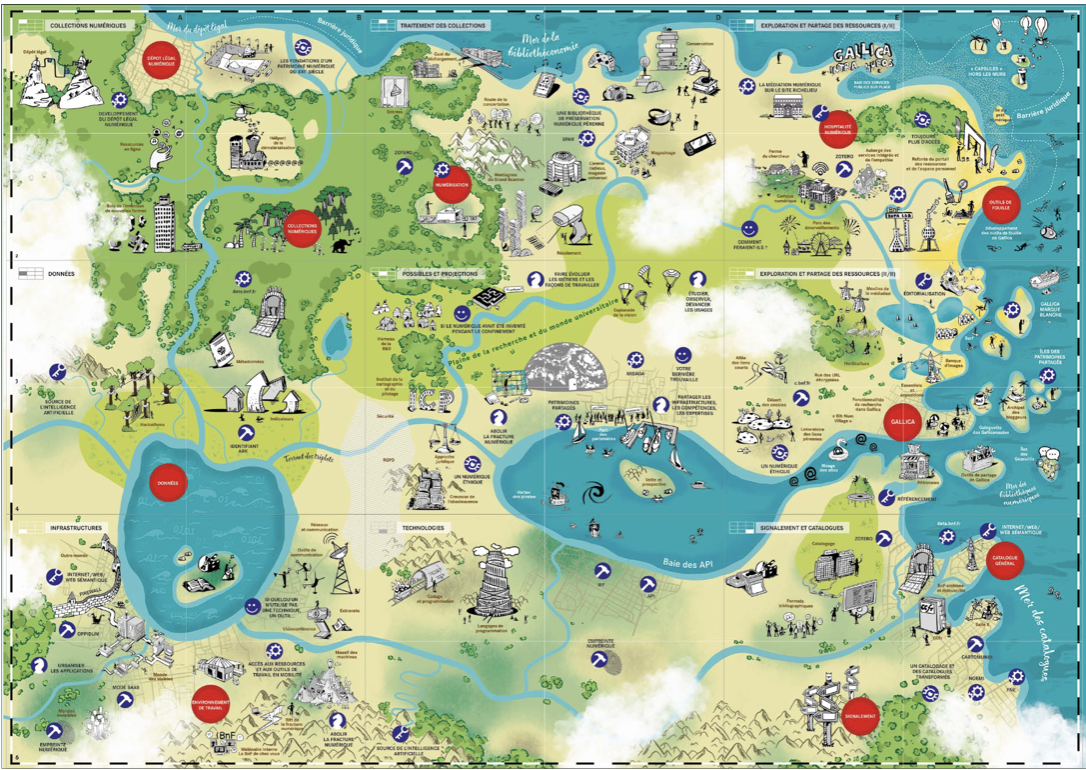
\includegraphics[width=\textwidth]{images/schema-bnf-num.png}
		\caption{Schéma numérique de la BnF. À voir en détail ici : 
			https://www.bnf.fr/fr/schema-numerique-bnf}
		\label{fig:monimage}
	\end{figure}
	

	La numérisation à la BnF ne s’est pas limitée à la simple reproduction numérique des collections existantes. Elle a également conduit à la création de véritables collections numériques. Cela impliquait non seulement de numériser des documents, mais aussi de repenser leur gestion, leur accessibilité, et leur valorisation sur le Web. Le projet Gallica, par exemple, a été un vecteur essentiel pour la diffusion des collections numérisées, tout en posant de nouveaux défis en termes de structuration et de gestion des données\footcite{bermes_numerique_2020} .
	
	Un des principaux défis identifiés est la pérennisation des collections numériques. Contrairement aux documents physiques, les objets numériques sont intrinsèquement volatils et nécessitent une attention constante pour garantir leur intégrité à long terme. La BnF a développé des stratégies spécifiques pour la conservation des collections nées numériques, intégrant des outils de gestion de données avancés et des partenariats avec des acteurs technologiques pour assurer la durabilité de ses archives numériques.
	
	L’impact de la numérisation sur la BnF est considérable, tant en termes de conservation du patrimoine que de diffusion de la culture. Avec plus de 9 millions de documents accessibles via Gallica, la BnF a réussi à toucher un public bien au-delà de ses frontières physiques, avec des millions de visites chaque année\footcite{engel_numerique_2022}. La numérisation a également permis de renforcer la coopération internationale, notamment à travers des initiatives telles que les bibliothèques numériques partagées et le BnF-DataLab, un laboratoire dédié à l’exploitation des données numériques.
	
	Cependant, cette transformation numérique n’est pas sans défis. Le passage au numérique a soulevé des questions complexes liées à la conservation à long terme des collections numérisées, à la gestion des droits d’auteur, et à l’équilibre entre l’accès libre aux documents et les exigences économiques des partenaires privés. La BnF a dû naviguer entre ces exigences parfois contradictoires, en développant des partenariats public-privé pour financer ses projets de numérisation tout en préservant l’accès public à ses collections\footcite{bruckmann_numerisation_2012}.
	
	Les projets de numérisation entrepris dans le cadre de ces partenariats ont été soigneusement évalués selon des critères incluant l’intérêt scientifique et culturel, la capacité à partager les investissements, ainsi que les conditions d’exclusivité temporaire pour garantir un retour financier. Ces initiatives témoignent de la capacité de la BnF à concilier ses ambitions culturelles avec les réalités économiques contemporaines\footcite{bruckmann_numerisation_2012}.
	\\

	À l’aube du XXIe siècle, l’ambition de la BnF de devenir un acteur central dans le paysage numérique mondial prend toute sa dimension. La création de Gallica, qui rassemble aujourd’hui des millions de documents, constitue une étape cruciale vers la réalisation de cette ambition\footcite{racine_bibliotheque_2011}. En parallèle, les efforts de la BnF pour adapter ses pratiques aux évolutions rapides des technologies numériques, tout en maintenant un lien étroit avec ses partenaires internationaux, montrent une institution en pleine mutation, résolument tournée vers l’avenir.
	
	Le rôle de la BnF dans le développement de l’économie numérique, à travers des projets comme “Alliance culture data”, illustre la prise de conscience de l’institution quant à l’importance de maîtriser les données culturelles à l’ère du numérique\footcite{engel_numerique_2022}. Ce projet, qui vise à créer une plateforme d’échanges de données culturelles, s’inscrit dans une stratégie plus large de renforcement de la souveraineté numérique française et européenne.
	
	\subsection{Les  collections numériques et leurs spécificités.}
	
	Avant d’entrer dans les collections de façon sommaire, définissons ce qu’est une collection « numérique ». Comme nous l’avons vu, la Bibliothèque nationale de France a joué un rôle pionnier dans le développement des collections numériques, marquant une étape cruciale dans la préservation et la diffusion du patrimoine culturel. Une collection numérique, bien qu’elle partage des objectifs communs avec les collections physiques, se distingue par sa nature dématérialisée et les opportunités uniques qu’elle offre en termes de connexions entre différents ensembles documentaires.
	
	Selon l’article “Le concept de collection numérique” de Frédéric Martin et Emmanuelle Bermès\footcite{martin_concept_2010}, les collections numériques ne se limitent pas à la simple reproduction de documents physiques. Elles exploitent les potentialités du numérique pour créer des ensembles cohérents à partir de ressources multiples et dispersées . Cela permet une flexibilité dans la gestion et la valorisation des collections, impossible à réaliser avec des collections physiques traditionnelles.
	\\
	
	La diversité des collections numériques de la BnF reflète l’ampleur et la richesse du patrimoine qu’elle conserve. Gallica, la principale bibliothèque numérique de la BnF, regroupe près de 10 millions de documents, allant des livres et journaux aux objets en 3D, en passant par les estampes, cartes, manuscrits et partitions \footnote{Les chiffres pour chaque catégorie sont : 5,8 millions de numéros de presse et de revues; 1,8 million d’images; 864 433 livres; 519 877 objets; 196 488 cartes; 186 507 manuscrits; 64 968 partitions; 52 004 enregistrements sonores; 5 585 vidéos. Chiffres présents sur https://gallica.bnf.fr/GallicaEnChiffres}. Ce projet montre comment la BnF a su élargir son offre numérique pour inclure une gamme de contenus de plus en plus diversifiés, répondant ainsi aux besoins variés de ses utilisateurs.
	
	En plus de Gallica, la BnF a développé des projets spécifiques tels que RetroNews, dédié à la presse ancienne avec plus de 20 millions de pages numérisées, et la Banque d’images, qui propose plus d’un million de dessins, affiches, et photographies\footcite{leroy-terquem_milles_2023}. Ces initiatives témoignent de l’engagement de la BnF à valoriser différents types de documents, en fonction des publics ciblés et des usages envisagés.
	\\
	
	La gestion des collections numériques nécessite une adaptation des pratiques bibliothéconomiques. Contrairement aux collections physiques, ces collections exigent des stratégies spécifiques pour leur sélection, leur conservation et leur mise à disposition en ligne. La numérisation de masse, par exemple, implique une sélection rigoureuse basée sur l’intérêt documentaire, l’état de conservation des documents, et les considérations juridiques, notamment en ce qui concerne les droits d’auteur .
	
	Pour garantir la pérennité des collections numériques, la BnF doit également adopter des stratégies de préservation numérique, telles que la migration des formats de fichiers et l’utilisation de métadonnées enrichies. Ces efforts visent à assurer que les documents restent accessibles et utilisables à long terme, malgré l’évolution rapide des technologies .
	\\
	
	Et l’un des défis majeurs des collections numériques est leur découvrabilité. Avec des millions de documents disponibles en ligne, la BnF doit s’assurer que ces ressources sont non seulement accessibles, mais également facilement repérables par les utilisateurs. La visibilité des collections en ligne dépend souvent des algorithmes des moteurs de recherche, ce qui rend crucial le rôle de la médiation numérique.
	
	Pour se faire, la BnF a mis en place des initiatives telles que data.bnf.fr, qui expose les données de la bibliothèque sur le web pour améliorer leur indexation par les moteurs de recherche. En parallèle, des sélections thématiques et des listes de publications périodiques ont été créées pour guider les utilisateurs à travers les vastes collections numérisées de la BnF .
	\\
	
	Après avoir exploré les défis et les stratégies liés à la gestion et à la médiation des collections numériques de la BnF, il est essentiel de se pencher sur une collection qui nous intéresse tout particulièrement : les manuscrits. Cette collection, riche et variée, dont dispose la BnF est particulièrement intéressante dans le cadre d’une mise en place d’un projet d’intelligence artificielle, et plus particulièrement d’un projet de reconnaissance optique d’écritures manuscrites. 
	
	Si nous nous penchons sur les chiffres de la BnF, et plus particulièrement de Gallica, la bibliothèque dispose de 186 507 manuscrits numérisés. Cependant, l’entrepôt OAI  (Open Archives Initiative) de la BnF, un système de gestion des métadonnées bibliographiques qui permet de centraliser et de standardiser l’accès à ces informations, après interrogation, nous renvoie un total de 203 252 documents reconnus comme des manuscrits. Mais dans ces deux cents trois mille documents, qu’avons nous concrètement ? 
	
	Après avoir extrait les métadonnées qui nous intéressent des différentes fiches XML (Extensible Markup Language) de l’OAI, il est possible d’en tirer une analyse et de pouvoir mettre en lumière différents corpus documentaires au sein même de la collection. Pour pouvoir comprendre clairement ce qu’il y a au sein de cette dernière, trois métadonnées vont être mises en valeur, ces trois même métadonnées qui sont à prendre en considération lorsque l’on veut planifier un projet HTR sur des documents pareils : La langue, la date ainsi que le type de numérisation. Néanmoins, même si cela est important, nous ne tiendrons pas compte des valeurs « nulles », comme des métadonnées non extraites ou non présentes dans les fiches; nous y reviendrons. 
	
	Tout d’abord, la richesse linguistique des manuscrits de la BnF. Sans grande surprise, puisqu’il s’agit d’un établissement jouant un rôle dans la préservation du patrimoine français, la langue française domine avec une présence de 58,6\% dans les manuscrits numérisés. Cependant, dans cette majorité de documents en français, seule la notion « fre » est prise en compte, mettant de côté d’autres documents en français représenté par « fro », pour français ancien, ou « frm » pour le français moyen. D’autres codes langues comme « fr. », « fra », « Fre » ou encore « fr » sont présents mais ne sont pas pris en compte. Le format Dublin Core utilisé à la BnF respecte la norme internationale ISO 639 qui définit des codes pour la représentation des noms de langues, facilitant ainsi la communication et l’échange de données linguistiques à l’échelle internationale\footcite{byrum_iso_1999}. Avec ces autres codes français, nous atteignons une part de document en français de 59,25\%. Le français ancien et moyen représentent respectivement 0,014\% et 0,0096\% des documents manuscrits de la BnF. 
	
	Au-delà de la prédominance du français, le latin occupe la deuxième place avec 11,2 \% des manuscrits, soulignant l’importance historique de cette langue dans les collections anciennes. Viennent ensuite les documents marqués par des “valeurs multiples” dans le XML (10,4 \%), ce qui reflète soit une diversité linguistique au sein d’un même document, soit des métadonnées non standardisées.
	
	L’arabe, avec 6 \%, et le chinois, avec 5,9 \%, représentent des parts significatives des collections, attestant de la diversité culturelle et géographique des manuscrits conservés par la BnF. D’autres langues, telles que le grec ancien (3,2 \%), l’hébreu (1,7 \%), l’italien (1,1 \%), le persan (0,8 \%) et le turc ottoman (0,8 \%), illustrent encore plus la richesse linguistique de cette collection.
	\\
	\begin{figure}[h!]
		\centering
		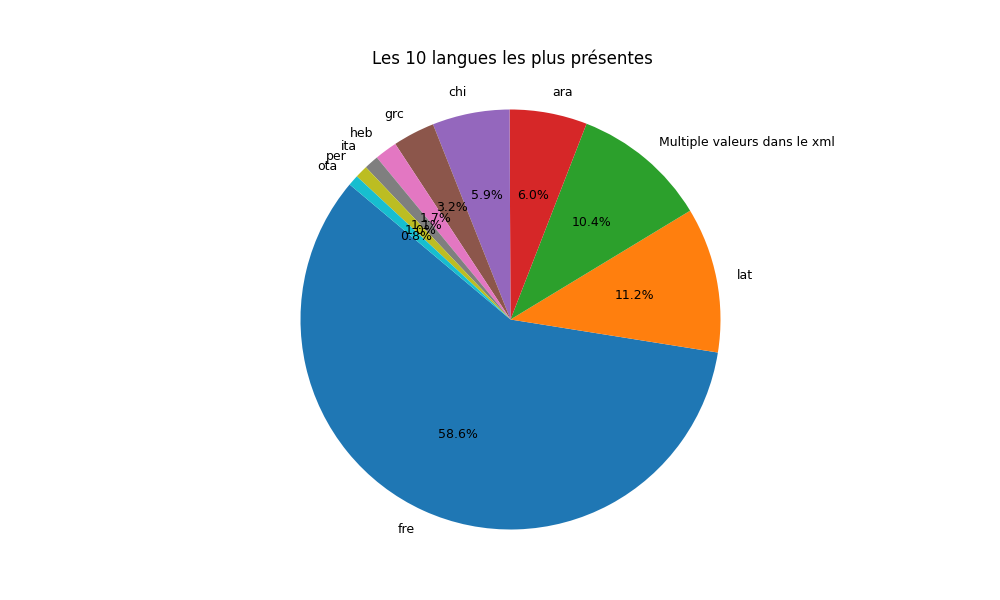
\includegraphics[width=0.8\textwidth]{images/langue_mss.png}
		\caption{Les 10 langues les plus présentes au sein des manuscrits de la BnF}
		\label{fig:monimage}
	\end{figure}
	En poursuivant l’analyse de la collection des manuscrits, penchons-nous sur les dates, et plus largement sur la répartition par siècle, afin de saisir la richesse temporelle de cette collection numérisée.
	Les documents les plus présents au sein des manuscrits numérisés de la BnF sont ceux du XXe siècle, représentant 34,1 \% de l’ensemble, suivis de près par ceux du XIXe siècle avec 27,7\% des manuscrits. Le XVIIIe siècle, bien que moins représenté, constitue tout de même 11,8 \% des manuscrits numérisés. Les périodes antérieures, du XVe au XVIIe siècle, sont également bien représentées, avec respectivement 5,5 \% pour les XVe et XVIIe siècles, et 4,8 \% pour le XVIe siècle.
	
	Enfin, les manuscrits datant des périodes médiévales et antérieures (Xe au XIVe siècle), bien que proportionnellement moins nombreux, constituent une partie précieuse de cette collection. Les pourcentages vont de 0,9 \% pour le Xe siècle à 4,2 \% pour le XIVe siècle. Cette analyse montre que, bien que les XIXe et XXe siècles soient les plus représentés, les siècles antérieurs, particulièrement ceux du Moyen Âge, restent d’une importance capitale pour la recherche historique, illustrant la profondeur temporelle et la richesse patrimoniale des collections manuscrites de la BnF. 
	\\
	\begin{figure}[h!]
		\centering
		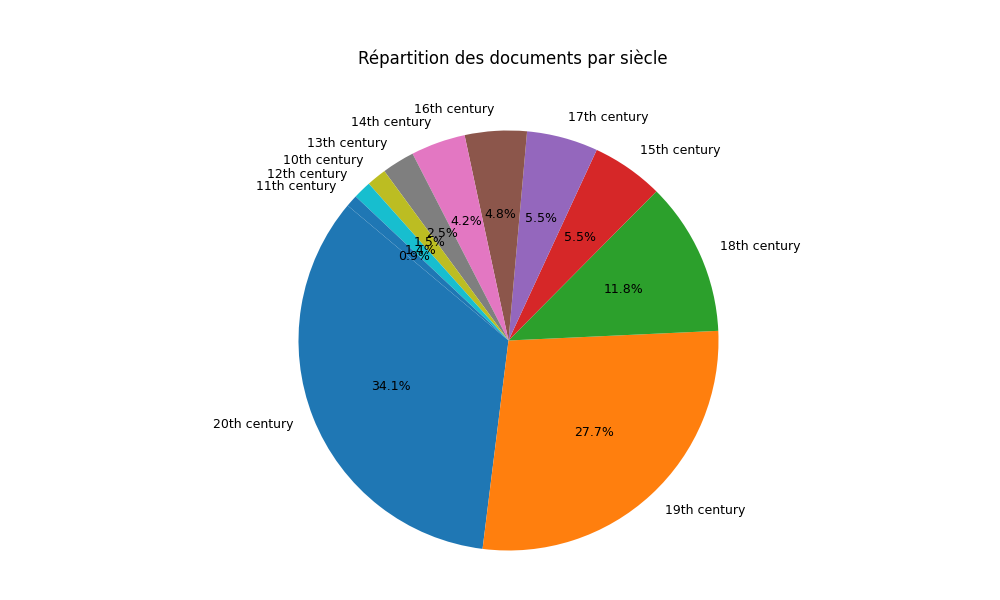
\includegraphics[width=0.8\textwidth]{images/siecle_mss_bnf.png}
		\caption{Les grandes périodes historiques présentes au sein des manuscrits de la BnF}
		\label{fig:monimage}
	\end{figure}
	
	Pour finir, un dernier point sur le type de document original utilisé par la BnF pour numériser ses manuscrits. La BnF numérise ses documents de deux manières.
	
	À partir d’un document original, un document physique que l’on a sorti des collections afin qu’il puisse subir une campagne de numérisation, permettant d’avoir un rendu de haute qualité mais aussi d’obtenir un document numérique le plus fidèle possible à l’original. Cette méthode, qui représente 55,5 \% des numérisations, garantit une reproduction fidèle des œuvres, préservant chaque détail, chaque texture et chaque nuance de l’original, tout en contribuant à la préservation à long terme des documents, en réduisant leur manipulation directe.
	\begin{figure}[h!]
		\centering
		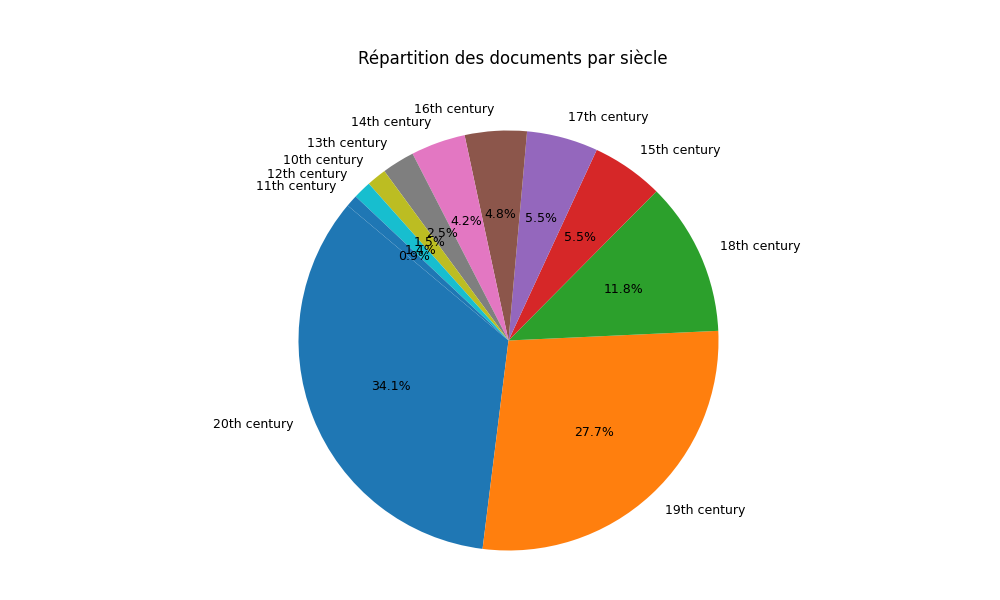
\includegraphics[width=0.8\textwidth]{images/siecle_mss_bnf.png}
		\caption{Répartition des différentes types de numérisations}
		\label{fig:monimage}
	\end{figure}
	Et à partir de documents de substitution, comme des microfilms ou des copies antérieures. Cette approche est adoptée principalement lorsque l’original est trop fragile pour être manipulé, ou lorsque son accès est restreint pour des raisons de conservation. Bien que cette méthode puisse ne pas capturer la même profondeur de détail que la numérisation directe de l’original, elle permet néanmoins d’assurer l’accessibilité numérique de ces documents tout en protégeant les originaux des risques d’usure ou de dégradation supplémentaires. Cette méthode ci représente 44,5\% des numérisations.
	\\
	
	Ces analyses permettent de mieux comprendre ce qu’il y a au sein d’une collection aussi riche et variée que la collection des manuscrits de la BnF. Et il s’agit seulement des documents numérisés. Cependant, il est important de noter que, pour ces trois métadonnées, l’on rencontre des données manquantes. Ceci est important de le mentionner car cela joue énormément sur les représentations statistiques. Par exemple, concernant les langues, 36,3\% des documents manuscrits numérisés de la BnF, soit 70 499 documents, n’ont pas de code langue attribué\footnote{Ou la valeur de la métadonnée n’a pas été extraite. Valable pour les dates ainsi que pour le type de numérisation.}. Et de même pour les deux autres métadonnées, pour les dates, c’est 51 043 documents qui n’ont pas de date, soit 34\%, et pour la numérisation c’est 59,5\% des documents qui n’ont aucune donnée sur le type de numérisation, soit 120 951 documents. 
	
	Connaître en détail les documents est important pour la mise en place d’une reconnaissance HTR efficiente. Contrairement à l’OCR, qui s’appuie sur un nombre limité de styles de caractères, l’HTR doit faire face à une diversité infinie d’écritures manuscrites, chaque main étant unique. Tandis que l’OCR fonctionne principalement avec des polices de caractères normalisées, l’HTR doit s’adapter à une variété immense de styles d’écriture manuscrite, qu’ils soient personnels ou institutionnels. Cette variabilité est particulièrement complexe à gérer, car elle dépend non seulement de l’individualité de chaque scribe, mais aussi des spécificités historiques et culturelles de chaque période.
	
	Par exemple, les écritures de chancellerie au Moyen Âge ou les écritures gothiques présentent des caractéristiques communes, souvent répliquées avec une certaine uniformité dans les documents de l’époque. Connaître ces particularités, repérables dans les métadonnées, notamment sous la balise <dc:format> des fiches XML de l’OAI, permet de regrouper les documents présentant des styles similaires. En identifiant des ensembles homogènes, tels que les manuscrits rédigés par un même auteur ou copiste, ou encore ceux réalisés dans un même contexte historique ou géographique, on peut ainsi affiner les modèles HTR pour qu’ils soient plus précis et adaptés à ces spécificités.
	
	Par ailleurs, certaines écritures ont traversé les époques avec des variations relativement mineures, ce qui permet de regrouper ces documents pour un traitement HTR plus cohérent et efficace. Les manuscrits rédigés dans un style gothique, par exemple, bien qu’ils puissent présenter des variations selon les régions et les périodes, partagent souvent une structure de base similaire. Regrouper ces documents sous un même projet HTR peut donc conduire à des résultats de reconnaissance plus fiables. 
	\\
	
	Outre le manque de données sur certains documents, qui rend leur traitement plus complexe en raison de l’absence d’informations cruciales comme la date ou la langue, la récupération des métadonnées peut également s’avérer ardue en raison de leur manque de normalisation. Si le code langue tend à respecter, dans une certaine mesure, les normes internationales ISO 639, il n’en va pas toujours de même pour les autres balises. Celles-ci sont souvent remplies en fonction des informations fournies par le conservateur, ce qui impose de rechercher l’information pertinente au milieu de nombreuses autres.
	\\
	
		\begin{figure}[h!]
		\centering
		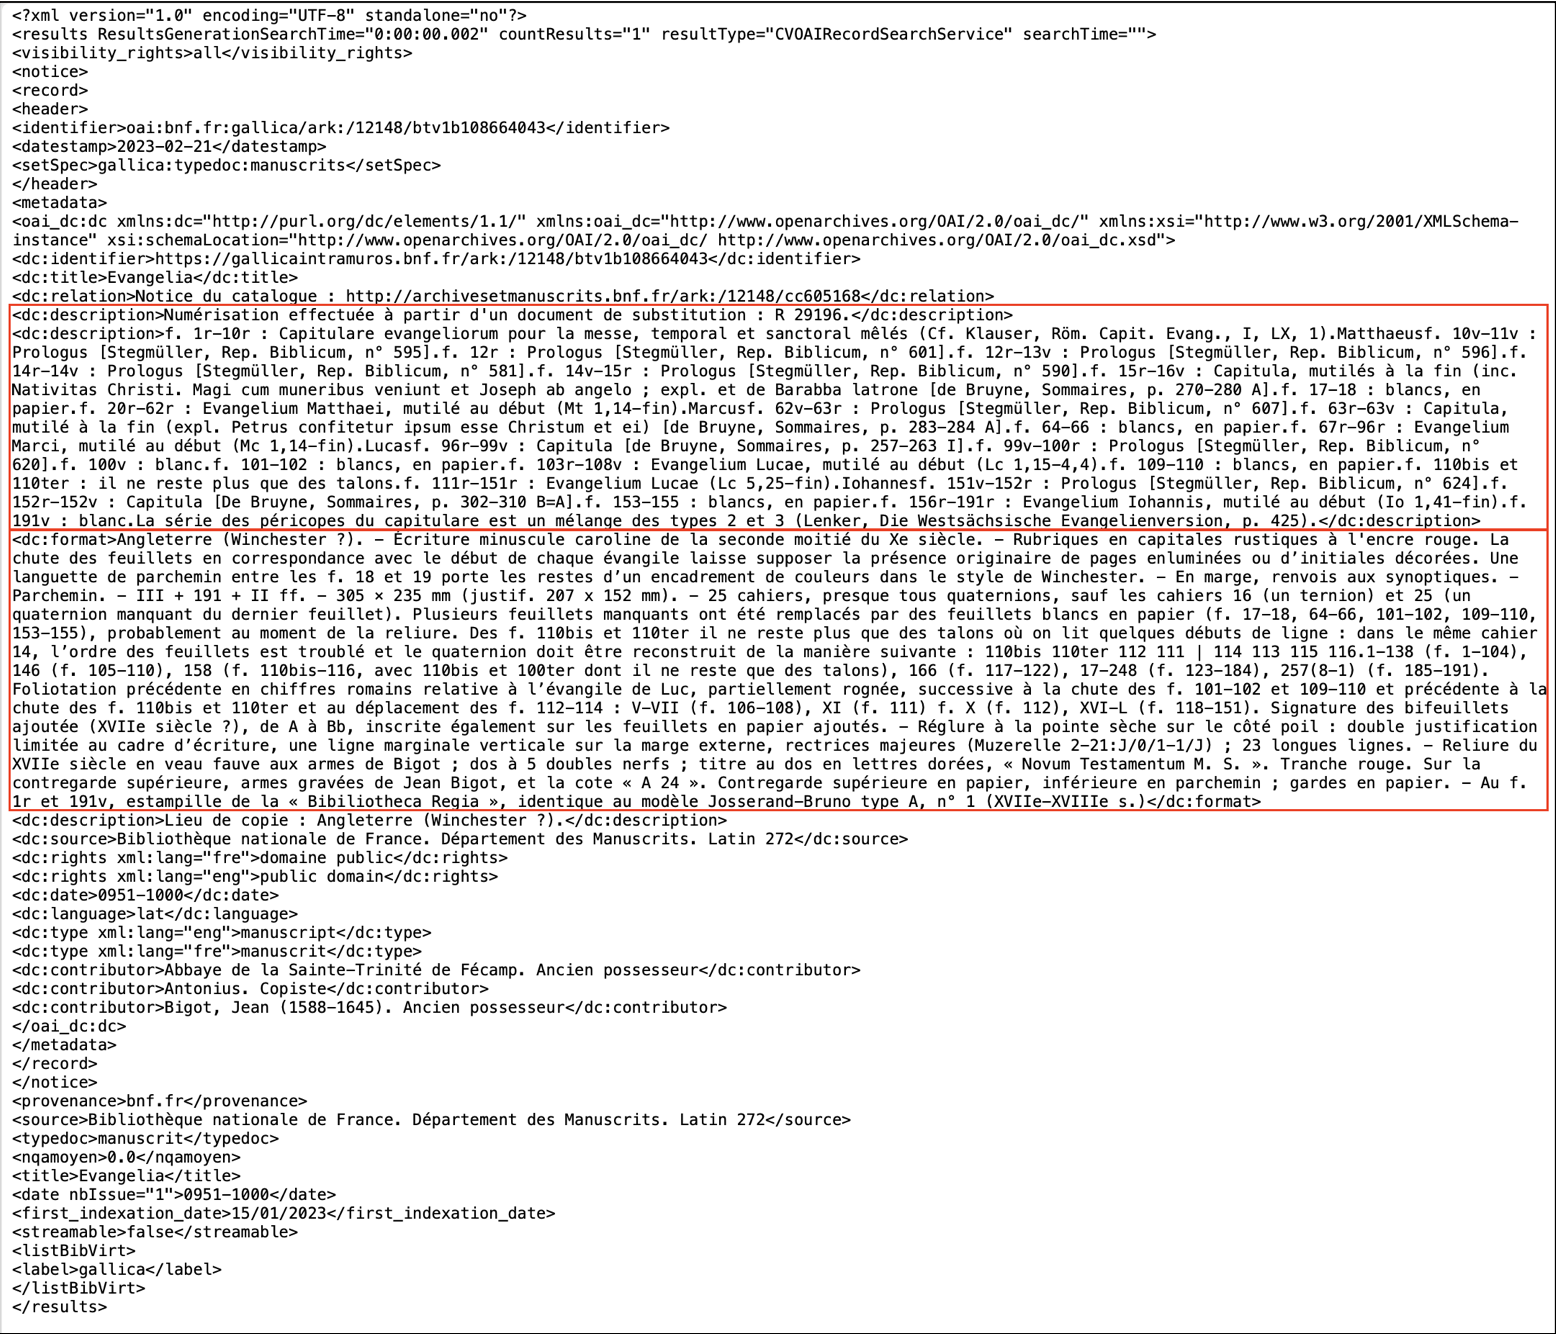
\includegraphics[width=0.8\textwidth]{images/fiche_xml_dc.png}
		\caption{Capture de la fiche XML OAI du manuscrit btv1b108664043}
		\label{fig:monimage}
		\end{figure}
	
	
	Par exemple, pour le document btv1b108664043, le style de numérisation est indiqué dans une balise <dc:description>, mais cette même balise contient également une deuxième occurrence avec des informations supplémentaires sur le manuscrit. De même, le style d’écriture est indiqué dans la balise <dc:format>, mais cette balise inclut également des détails matériels sur le document, ce qui complique l’extraction ciblée des informations nécessaires. Cette variabilité dans la structure et le contenu des métadonnées souligne la nécessité de procédures adaptées pour analyser et utiliser ces données efficacement dans le cadre d’un projet HTR.
	
	\subsection{La maîtrise des métadonnées : clé de la réussite ?}
	En somme, la numérisation des collections de la BnF, en particulier des manuscrits, a mis en lumière l’importance de maîtriser les métadonnées et de comprendre les spécificités de chaque document pour assurer la mise en place d’un projet de reconnaissance efficace des écritures manuscrites. Si la diversité et la richesse de ces collections numériques offrent des opportunités immenses pour la recherche et la préservation, elles posent également des défis considérables, notamment en matière de normalisation des métadonnées et de gestion de la variabilité des styles d’écriture. C’est précisément cette complexité qui nécessite une chaîne de traitement OCR et HTR rigoureuse et bien pensée. À présent, il convient de se pencher sur l’organisation interne de la BnF et les collaborations essentielles qui sous-tendent la réussite d’un projet de reconnaissance des écritures manuscrites. Comprendre comment les différents services collaborent, comment les processus sont structurés, et comment ces dynamiques organisationnelles permettent de mettre en œuvre efficacement les technologies d’intelligence artificielle et de reconnaissance optique, est crucial pour saisir l’ampleur des défis et des solutions apportées dans la gestion des manuscrits numérisés de la BnF.
	
	\part{Deuxième partie}
	\chapter{Organisation et Collaboration.
		La BnF, une fourmilière patrimoniale.}
	
	\lettrine{L}a collaboration, le fait que des équipes entières travaillent main dans la main afin d’avancer sur un projet commun est une pierre angulaire de toute structure, qu’elle soit une institution patrimoniale ou non. Et cela est d’autant plus vrai lorsque l’on parle de l’implémentation d’un projet d’intelligence artificielle au sein de ces institutions. Pour pouvoir mettre en place et faire en sorte que le projet d’intelligence artificielle, visant à traiter une masse de données importante, fonctionne, il faut une organisation et une collaboration entre différents services et différents acteurs au sein de l’organigramme. Pour illustrer ces propos, la BnF est un très bon exemple de complexité en terme d’organigramme et n’échappe pas à la règle de la collaboration concernant le fonctionnement de sa chaîne de traitement interne. 
	
	\subsection{L’Organisation interne de la chaine OCR de la BnF}
	
	La chaine de traitement de reconnaissance de caractères optiques de la BnF nécessite la collaboration de différents services, composés eux-même de différents bureaux, afin que la chaine fonctionne correctement, de l’entrée des documents à la sortie de ces derniers. Pour ce faire, illustrons ces propos par le biais de la présentation de la chaine OCR à échelle humaine \footnote{cf. Annexe Schéma \ref{fig:schemorganbnf}.} 
	
	Un descriptif complet de l’organigramme de la Bibliothèque Nationale n’est pas nécessaire pour cet exemple, ce qui est intéressant ici, c’est l’interactivité humaine à l’échelle de la chaine OCR. Tout au long du processus d’océrisation, ces entités et leurs bureaux vont être amenés à coopérer. Ici aussi, les principes du MLOps sont respectés. 
	En effet, la collaboration est un élément clé dans l’implémentation des systèmes MLOps, nécessitant la participations d’une équipe multidisciplinaire, ici à la BnF, ceci est mis en avant avec la présence des équipes métiers, techniques et de production, des spécialistes de la numérisation ainsi que le département des collections qui ont pour mission la collecte, le catalogage et la conservation des différentes collections de la BnF (manuscrits, monnaies, photographies, imprimés, etc). Et ces rôles sont cruciaux pour concevoir, gérer, automatiser et exploiter les projets d’IA. Cela permet à l’institution de surmonter les défis liés à la gestion et à l’opération de systèmes de Machine Learning (ML)\footcite{kreuzberger_mlops_2023}. 
	
	Le travail autour de la chaine OCR est clairement définis et chaque équipes, chaque bureaux a une tâche particulière pour toutes les grandes étapes du fonctionnement de l’océrisation\footcite{bnf_printemps_2024}. Les équipes fonctionnelles jouent un rôle central en début de chaîne, en recensant les besoins et en paramétrant les prestations. Elles sont responsables du suivi des tests et de la gestion des anomalies, garantissant ainsi que les spécifications techniques et les exigences des projets soient respectées.
	
	Parallèlement, les équipes de production assurent le maintien des applications utilisées tout au long du processus. Elles sont en charge de la transformation des images et de la génération des paquets, tout en gérant les erreurs et anomalies qui peuvent survenir. Elles supervisent également l’aspect technique des envois de bordereaux, veillant à ce que les flux de données soient bien organisés et que les informations soient correctement transmises. Ces équipes utilisent des outils tels que SchedulingTools, et SuiviNum pour faciliter leurs tâches. Le service de numérisation, quant à lui, est responsable du suivi des demandes de numérisation, assurant une mise à disposition régulière et une livraison efficace des documents numérisés. Ce service coordonne également le contrôle des dépôts, vérifiant que les documents sont correctement stockés et accessibles. Les outils métiers utilisés, comme NUM-G027 et SIPIL-NUM, permettent de suivre l’état des numérisations et de gérer les aspects logistiques.
	
	Enfin, le département des collections, et plus précisément la DCO, joue un rôle crucial dans la validation et la conservation des contenus numérisés. Ce département effectue le contrôle qualité des collections numérisées, transmet les demandes de réfection si nécessaire, et s’assure que les métadonnées bibliographiques sont précises et complètes. Cette phase est essentielle pour garantir la qualité et la fiabilité des données mises à disposition des utilisateurs.
	\\
	
	Cette interaction, si elle est visible et concrète pour une chaîne à échelle industrielle comme la chaîne OCR, elle est aussi visible pour une chaîne à échelle plus réduite comme celle de l’HTR. 
	
	En effet, pour mettre en place la chaîne HTR, il est tout aussi important de collaborer avec des acteurs et des départements variés afin de pouvoir proposer les meilleurs résultats possibles. Et pour cela, en début de projet, la rencontre avec un ingénieur d’étude du DataLab, spécifiquement recruté pour faire l’interface entre la TGIR (Très grande Infrastructure de Recherche) Huma-Num et le DataLab de la BnF\footcite{carlin_bnf_2021}, a été nécessaire. Cet ingénieur apporte une expertise technique et scientifique précieuse, notamment en matière de renforcement des API et de mise en place d’une infrastructure numérique spécifique, indispensable pour gérer efficacement les collections sous droits tout en respectant les contraintes de sécurité imposées par la BnF. Cette collaboration, en plus d’offrir un soutien technique, permet d’assurer que les infrastructures numériques sont adaptées aux besoins spécifiques des projets de recherche, comme ceux dédiés à la reconnaissance manuscrite.
	
	De plus, une collaboration avec le Département des Manuscrits a été nécessaire lors de la conception de la chaine. Cette collaboration s’est faite au travers d’un échange avec des spécialistes du manuscrits concernant les métadonnées de ces derniers, afin de savoir quelle métadonnée était intéressante parmi toutes celles disponibles dans les fiches XML de l’OAI et afin de savoir où trouver les bonnes informations. Par exemple, puisque les données ne sont pas normalisées, les conservateurs ont pu renseigner des informations intéressantes dans une balise avec d’autres informations, comme la balise description qui est une balise aux informations larges, mais où l’on peut trouver si le document est numérisé à partir d’un original ou d’un document de substitution (donc à comprendre un micro-film).  
	\\
	
	L’interaction entre ces différents services et bureaux illustre parfaitement l’application des principes de MLOps à la BnF. En combinant l’expertise technique, la gestion des processus et la conservation des collections, l’institution parvient à gérer efficacement les projets de numérisation, d’OCR et de HTR, surmontant ainsi les défis techniques et organisationnels inhérents à ces initiatives. La collaboration étroite entre les équipes fonctionnelles, les équipes de production, le service de numérisation et le département des collections permet non seulement d’assurer une production continue et de haute qualité, mais aussi de maintenir une flexibilité et une adaptabilité face aux évolutions technologiques et aux besoins des utilisateurs.
	
	La BnF a décidé l’internalisation de sa chaîne de reconnaissance optique pour différentes raisons. Tout d’abord, la question du traitement des documents provenant de différentes filières, cela permet à la BnF de gérer les documents provenant d’ateliers internes, de partenaires ou encore de projets rétrospectifs qui ne sont pas couverts par les marchés courants de numérisation, sans oublier le traitement du service à la demande afin de pouvoir répondre à des besoins spécifiques, parfois urgents, des gallicanautes. Posséder une chaine OCR internet permet aussi de pouvoir avoir un regard sur le suivi de la qualité des OCR produits ainsi que sur les taux de confiance des moteurs, enregistrés dans une base de données dans le but d’interroger et requêter cette dernière\footcite{bnf_printemps_2024}.  De plus, la reconnaissance optique est une technologie mature, certaines institutions l’intègrent automatiquement dans la chaine lorsqu’ils décident de mettre en place un projet de numérisation, comme la National Library of Norway qui introduit l’océrisation dans sa numérisation de ses corpus à partir de 2006\footcite{solbakk_implementation_nodate}. Cependant, la reconnaissance manuscrite est une technologie encore récente et peu de bibliothèque ont un traitement HTR dans la chaine de numérisation de leur collection de manuscrits.
	
	\subsection{Vers une externalisation ? }
	
	Les institutions patrimoniales peuvent faire appel à des prestataires extérieurs spécialisés dans la reconnaissance manuscrite afin de mener à bien certains projets sur leurs collections. Ces collaborations permettent d’accéder à des technologies avancées et à une expertise spécialisée qui ne sont pas toujours disponibles en interne.
	\\
	
	Par exemple, le projet HUGIN-MUNIN\footnote{ https://hugin-munin-project.github.io/} en Norvège illustre parfaitement comment les bibliothèques et institutions culturelles peuvent s’associer à des communautés de recherche pour développer des technologies de reconnaissance de texte manuscrit à grande échelle. L’objectif principal de ce projet est de créer de nouveaux modèles de réseaux neuronaux profonds, robustes et généralisables, qui permettront d’intégrer l’HTR dans le processus standard de numérisation des collections des institutions culturelles norvégiennes. Ce projet, mené en collaboration par TEKLIA\footnote{ Compagnie française proposant des solutions pour la reconnaissance de texte (OCR/HTR) ainsi que d’autres prestations (extractions d’informations, analyse de structure ou classification de documents).} et la National Library of Norway, vise à minimiser le besoin d’annotations manuelles continues et d’entraînement de modèles, en s’appuyant sur des techniques d’apprentissage actif, non supervisé, de transfert, et de zéro-coup. La réussite de ce projet repose sur une collaboration interdisciplinaire entre des communautés de recherche spécialisées en analyse de documents et en HTR, tant au niveau national qu’international. Grâce à cette approche, le projet HUGIN-MUNIN contribuera à enrichir l’expertise norvégienne en systèmes autonomes et intelligence artificielle, tout en renforçant le potentiel d’innovation du secteur culturel norvégien par le transfert de connaissances et de bonnes pratiques. Il est possible, notamment, de parler du projet BALSAC\footcite{vezina_overview_2020}, qui vise à construire une base de données des événements démographiques (naissances, mariages et décès) de la population du Québec en reliant ensemble les informations issues des registres paroissiaux transcrits. Cette base de données comprend environ 2 millions d’images numérisées de registres paroissiaux manuscrits, datant principalement de la seconde moitié du XIXe siècle jusqu’au début du XXe siècle. Pendant plus de 40 ans, ces manuscrits ont été laborieusement transcrits à la main par les chercheurs du projet, un travail colossal et chronophage. Grâce à l’intervention de TEKLIA, il a été possible d’accélérer considérablement ce processus. TEKLIA a développé un système capable de transcrire automatiquement ces pages manuscrites, de les segmenter en actes individuels, de détecter les entités importantes (comme les noms et les dates), et d’exporter les résultats sous forme de fichiers XML. Ces fichiers sont ensuite intégrés dans la base de données BALSAC, où l’équipe peut les utiliser pour reconstituer des biographies individuelles et des histoires familiales complètes. Cette collaboration a permis à la Bibliothèque et Archives nationales du Québec (BAnQ) de valoriser son vaste corpus documentaire, le rendant plus accessible aux chercheurs et au grand public. Les chercheurs du projet BALSAC ont aussi utilisé la plate-forme Transkribus\footnote{ Plate-forme de reconnaissance de texte et de transcription automatique pour les documents historiques, développée par l'Université d'Innsbruck et actuellement gérée par READ-COOP.} pour la vérité de terrain. 
	
	En outre, des outils comme Transkribus sont de plus en plus adoptés par des bibliothèques à travers le monde pour faciliter la numérisation et la transcription de leurs collections manuscrites. Par exemple, la Bibliothèque nationale de Serbie a intégré Transkribus dans son processus de numérisation pour améliorer la reconnaissance automatique des textes manuscrits\footcite{malesev_need_2022}. Cet outil permet aux institutions de bénéficier d’une technologie avancée de HTR sans avoir à développer des solutions en interne. En utilisant Transkribus, la Bibliothèque nationale de Serbie et d’autres institutions similaires peuvent non seulement accélérer le processus de numérisation, mais aussi améliorer la qualité et l’accessibilité des documents numérisés pour les chercheurs et le grand public.
	
	Dans le cadre de la BnF, la chaine de traitement HTR pourrait être en partie externalisée en faisant appel à des technologies de partenaires privés comme TEKLIA ou READ (Transkribus), le tout, en gardant le contrôle sur les processus et les résultats. Les prestataires externes interviendrait sur l’entrainement des modèles adaptés aux différents types de manuscrits de la BnF ainsi que sur la segmentation précises des documents, ou encore l’extraction des entités (noms, dates, etc) pour mettre en valeur des données, tout en produisant des fichiers XML ALTO afin de fournir des transcriptions sur la bibliothèque numérique.
	\\
	
	Néanmoins, externaliser la chaîne par le biais d’un prestataire comme TEKLIA n’est pas la seule option envisageable pour la BnF. L’un des piliers du succès de toute entreprise, y compris dans le domaine de la recherche, est la collaboration. La BnF l’a bien compris et, à travers son DataLab\footcite{carlin_bnf_2021}, elle met en place un écosystème propice à l’innovation en matière d’humanités numériques. Le DataLab, comme mentionné précédemment, joue un rôle clé en fournissant un environnement technique et scientifique favorable à la mise en place de chaînes de traitement telles que celle de l’HTR. Ce service, en partenariat avec Huma-Num, permet non seulement de bénéficier de l’expertise de spécialistes en ingénierie des données, mais aussi de collaborer avec des chercheurs extérieurs pour développer des solutions sur mesure adaptées aux besoins spécifiques des projets de la BnF.
	\\
	
	Cette coopération va au-delà d’un simple soutien technique. Les appels à projets du DataLab permettent aux chercheurs de travailler en immersion sur les collections numériques de la Bibliothèque, souvent pour des périodes allant jusqu’à dix-huit mois. Durant cette période, la BnF ne se contente pas de fournir un accès aux données ; elle finance et accompagne activement les chercheurs, leur permettant d’expérimenter, d’innover et de développer des outils qui bénéficieront à la fois à leur propre recherche et aux objectifs institutionnels de la Bibliothèque.
	
	Penchons nous sur quelques exemples de projets menés à la BnF. 
	\\
	
	Le projet READ CHINESE\footcite{bui_recognizing_2023} est un excellent exemple de la dynamique collaborative entre la BnF et une équipe de recherche spécialisée en intelligence artificielle. Ce projet a pour objectif de développer une chaîne de traitement pour la transcription automatique des manuscrits chinois, notamment ceux de la collection Pelliot de Dunhuang. Ces manuscrits, rédigés en sinogrammes, posent un défi particulier en raison de la complexité et de la diversité des caractères chinois anciens. Pour surmonter ces obstacles, l’équipe utilise des technologies avancées telles que TrOCR\footcite{li_trocr_2023} (Transformer-based OCR), un modèle de reconnaissance optique de caractères basé sur l'apprentissage profond, ou deep learning.
	\\
	
	Développé par Microsoft, TrOCR combine les capacités des modèles Transformer – largement utilisés dans le traitement automatique du langage naturel – avec les besoins spécifiques de la reconnaissance de caractères non latins, comme le chinois. Grâce à l’infrastructure fournie par le DataLab, TrOCR est entraîné et optimisé sur des corpus issus des collections de la BnF, assurant une reconnaissance précise des sinogrammes dans ces manuscrits anciens. Pour segmenter les documents complexes, le projet fait également appel à l’architecture Swin-Transformer, un modèle puissant de reconnaissance d’images. Le Swin-Transformer segmente les images en petites fenêtres, permettant de traiter localement les zones de texte grâce à une approche appelée “fenêtres décalées”\footcite{liu_swin_2021}. Cette méthode améliore la précision de la segmentation dans des manuscrits denses, renforçant l’efficacité globale du projet et la valorisation des collections historiques de la BnF.
	\\
	
	Un autre projet significatif est le Projet HTR Dulaurier. Ce dernier vise  à valoriser un ensemble de manuscrits arméniens conservés à la Bibliothèque nationale de France, connus sous le nom de fonds Dulaurier, du nom d’Édouard Dulaurier, un éminent érudit du XIXe siècle qui a largement contribué à la collecte et à l’étude des textes arméniens. Ce fonds est particulièrement riche en documents historiographiques et en recueils de correspondances, couvrant une période allant du VIIIe au XVIIIe siècle. Les manuscrits étudiés dans ce projet incluent des œuvres importantes telles que l’Histoire des guerres et des conquêtes des Arabes en Arménie de Łevond, l’Histoire de l’invasion du Caucase par les Mongols de Kirakos Ganjakec’i, et des chroniques rédigées par Abraham III Kretac‘i, parmi d’autres. Ces textes constituent une ressource inestimable pour les chercheurs s’intéressant à l’histoire et à la culture du monde arménien médiéval\footcite{coulie_valorisation_2022}.
	
	Le projet propose de traiter 14 manuscrits, représentant un total de 3960 pages, en utilisant des technologies de reconnaissance de texte manuscrit spécialement adaptées aux particularités de l’écriture arménienne. En raison de la complexité de ces manuscrits, souvent rédigés dans une écriture cursive difficile à déchiffrer, le projet met en œuvre une approche hybride combinant des méthodes basées sur des règles linguistiques et des réseaux de neurones. Cette combinaison vise à améliorer la précision de la transcription, avec un objectif de taux d’erreur inférieur à 3\%. Les résultats du projet seront intégrés dans plusieurs plateformes, notamment Gallica pour une recherche en texte intégral, et des interfaces dédiées telles que celles développées par GREgORI\footnote{Projet, initié par l’institut orientaliste de l’Université catholique de Louvain, visant à créer des concordances lemmatisées et des outils linguistiques pour les textes grecs et orientaux anciens, en étendant son champ d’application à plusieurs langues du christianisme oriental, tout en fournissant des ressources essentielles pour le traitement automatique du langage naturel. Kindt (Bastien), « Du texte à l’index. L’étiquetage lexical du De Septem Orbis Spectaculis de Philon le Paradoxographe : méthode et finalité » (2021). URL : \url{https://www.persee.fr/doc/ista_0000-0000_2021_act_1521_1_3881}.} et DALiH\footnote{ Projet «Digitizing Armenian Linguistic Heritage: Armenian Multivariational Corpus and Data Processing » visant à créer une plate-forme numérique open-source pour toutes les variétés de l’arménien, incluant des corpus textuels annotés et des modèles de traitement automatique du langage pour une langue multivariée peu dotée. https://anr.fr/Projet-ANR-21-CE38-0006} pour l’analyse linguistique et la comparaison de corpus.
	\\
	
	Enfin, le Projet HTRomance\footcite{clerice_htromance_2022} se concentre sur le développement et l’application de technologies de reconnaissance de texte manuscrit adaptées aux manuscrits en langues romanes. Porté par une équipe multidisciplinaire incluant des chercheurs de l’École nationale des chartes, INRIA, et plusieurs autres institutions académiques européennes, ce projet s’attache à traiter des manuscrits conservés dans différentes institutions patrimoniales, et rédigés dans diverses langues romanes, telles que le français, l’occitan, l’italien et l’espagnol. Ces manuscrits, qui couvrent des périodes historiques variées, présentent des caractéristiques linguistiques et paléographiques complexes, ce qui rend leur traitement particulièrement exigeant.
	
	Le projet vise à adapter et à spécialiser les modèles HTR existants pour les particularités des écritures romanes, en tenant compte des variations linguistiques régionales et historiques. En outre, le projet prévoit la création d’une base de données interrogeable, permettant aux chercheurs d’accéder facilement aux transcriptions et aux analyses linguistiques des textes. Cette base de données sera intégrée à des plateformes de recherche linguistique, facilitant ainsi la comparaison de textes, l’étude des variations linguistiques, et l’analyse philologique des manuscrits.
	\\
	
	\subsection{Les défis organisationnels et les solutions possibles.}
	
	Si la BnF coopère avec le monde de la recherche en mettant à disposition des services pour les chercheurs au travers de son DataLab, ces derniers, en contre partie, apportent une contribution significative à la Bibliothèque en termes de valorisation, d’accessibilité, et de préservation de ses collections patrimoniales. Chacun de ces projets, READ CHINESE, Dulaurier, et HTRomance, en s’appuyant sur des technologies avancées de reconnaissance de texte manuscrit et d’analyse linguistique, transforme des documents historiques complexes en ressources numériques accessibles et interrogeables, tout en enrichissant l’écosystème numérique de la BnF par des livrables techniques et des actions de formation.
	
	Le projet READ CHINESE offre à la BnF la possibilité de transcrire automatiquement des manuscrits chinois anciens, en particulier ceux de la collection Pelliot de Dunhuang. En plus des fichiers XML ALTO, qui seront intégrés à Gallica pour rendre ces textes plus accessibles aux chercheurs du monde entier, le projet développe et met à disposition des outils spécifiques de reconnaissance, permettant de traiter efficacement les sinogrammes anciens. Ces outils seront accompagnés d’un atelier de formation, réunissant les équipes du projet et celles du DataLab, et ouvert à la communauté des chercheurs intéressés par l’HTR du chinois, renforçant ainsi la diffusion des connaissances et l’application de ces technologies à d’autres projets.
	
	Le projet Dulaurier valorise les manuscrits arméniens en appliquant des techniques de reconnaissance de texte manuscrit, permettant ainsi de rendre ces documents accessibles non seulement aux spécialistes, mais aussi à un public plus large. Les productions HTR, notamment les fichiers XML ALTO, seront reversées à la BnF pour intégration dans des plateformes comme Gallica. De plus, les résultats du projet seront mis à disposition en accès ouvert, ce qui permettra de soutenir le développement de solutions intelligentes d’analyse ou l’enrichissement de systèmes existants. Le projet est également axé sur le transfert de connaissances, avec Calfa\footnote{  Start-up française dédiée au traitement automatique des langues orientales et à l’analyse automatisée de documents, incluant la reconnaissance de texte manuscrit et l’extraction d’informations. Elle conçoit des systèmes intelligents pour les acteurs du patrimoine, qu’ils soient du secteur public ou privé, ainsi que pour ceux engagés dans la numérisation de documents et de collections.} et GREgORI organisant des ateliers pour former la communauté scientifique, y compris les chercheurs et les bibliothécaires, aux bonnes pratiques en matière de paléographie numérique.
	
	Le projet HTRomance enrichit la BnF en développant des modèles HTR spécifiques aux langues romanes, ainsi que des modèles de segmentation pour YALTAi\footcite{clerice_you_2023}, outil permettant d’intégrer YOLO, un détecteur d’objet en temps réel, dans le moteur Kraken afin de segmenter les documents manuscrits et convertir les modèles, optimisant ainsi leur traitement et reconnaissance automatique. Ces modèles seront publiés et intégrés dans le moteur Kraken, renforçant ainsi les capacités techniques de la BnF pour traiter une diversité de manuscrits en langues romanes. En outre, le projet prévoit des formations au DataLab, incluant des sessions sur eScriptorium, une application open source développée depuis 2019 qui fournit une interface graphique pour le moteur Kraken, permettant de gérer l’ensemble du processus de transcription, du traitement de l’image à l’exportation des données\footcite{chague_escriptorium_2022}. Destinées aux médiévistes et modernistes, ces sessions seront accompagnées d’expériences sur la lisibilité des manuscrits. Ces initiatives, en partenariat avec le DataLab, visent à transférer les connaissances acquises et à accélérer la transition numérique des collections de la BnF.
	\\
	
	En somme, les collaborations entre la BnF et des partenaires extérieurs, qu’il s’agisse de chercheurs ou de prestataires spécialisés en HTR, comme TEKLIA, montrent clairement que l’externalisation partielle ou la coopération scientifique peut enrichir et accélérer la valorisation des collections patrimoniales. Ces projets démontrent l’importance d’intégrer des technologies avancées et des expertises externes pour transformer des documents historiques complexes en ressources numériques accessibles et interrogeables. Cependant, il est tout aussi essentiel de comprendre comment ces innovations s’intègrent dans l’écosystème de la BnF et de voir comment l’institution gère ses propres chaînes de traitement (OCR/HTR) en interne, garantissant ainsi une gestion efficace et une continuité de qualité dans ses processus de numérisation et de traitement des collections manuscrites.
	
	\part{Troisième Partie}
	\chapter{Les Chaines OCR et HTR,
		Architecture et déploiement des pipelines}
	
	\lettrine{L}a Bibliothèque Nationale de France  a mis en place une chaîne de traitement OCR interne, visant à produire son propre OCR sur ses documents numérisés. Cette initiative permet de pouvoir enrichir les documents numériques avec des données textuelles exploitables, afin de faciliter la recherche ainsi que la consultation. Le processus de l’OCR repose sur différentes étapes clefs passant de la sélection des documents au traitement OCR, et est structuré autour de critères rigoureux et d’une organisation soignées. Pour optimiser ces processus et assurer une gestion efficace, la BnF a intégré les principes de MLOps (Machine Learning Operations). MLOps permet d’automatiser et d’orchestrer les différentes étapes du traitement OCR et HTR, depuis la sélection des documents jusqu’à la mise en production des modèles et leur maintenance.
	
	\subsection{La Chaine OCR : Architecture et déploiement.}
	
	Avant de pouvoir commencer tout traitement OCR, les équipes du BCN, bureau chaine numérique, de la BnF passent par l’application DispoDocNum, afin de sélectionner les documents et de les regrouper selon des critères spécifiques, permettant ainsi de déterminer les priorités et d’optimiser le processus de traitement. 
	Pour cela, deux principaux modes de traitement existent : le traitement courant et le traitement rétrospectif.
	
	\begin{itemize}
		\item \underline{Traitement courant} : Ce mode de traitement consiste simplement à appliquer de l’OCR sur des documents récemment numérisés par les prestataires de la BnF. On y applique une période d’attente avant de procéder à l’OCR, permettant une gestion fluide et continue des flux de documents. \\
		\item \underline{Traitement rétrospectif} : Ce mode de traitement consiste à ajouter de l’OCR sur des documents déjà numérisés présents dans les catalogues, mais aussi sur des documents bien plus anciens de la BnF.  
	\end{itemize}
	
	Un intervalle de traitement est établi manuellement par les équipes pour optimiser la gestion des flux documentaires. Cette approche vise à prévenir toute surcharge ou, à l'inverse, tout ralentissement excessif du traitement. L'objectif principal est de maintenir un flux constant et efficace. Il convient de noter que la Bibliothèque nationale de France traite en moyenne environ 5 000 documents par jour. Cette donnée souligne l'importance d'une gestion rigoureuse du flux documentaire.
	
	La définition de l'intervalle de traitement s'adapte à la nature des prestations. Pour les prestations s'étendant sur plusieurs mois, il est possible de traiter les documents quotidiennement. En revanche, pour les prestations couvrant une ou plusieurs années, un intervalle spécifique est mis en place. Par exemple, pour l'année 2021, on pourrait instaurer un intervalle de trois jours, permettant ainsi de traiter les documents du 1er au 3 janvier, puis du 4 au 6 janvier, et ainsi de suite.
	\\
	
	Une prestation de numérisation, identifiée par un numéro unique (par exemple 115, 706, 219), représente un ensemble cohérent de documents à numériser. Cette prestation peut être réalisée soit par un prestataire externe, soit par un atelier interne de la BnF. Chaque prestation correspond à un type spécifique de documents (comme des monographies, des périodiques, ou des manuscrits) et à un prestataire particulier. Cette organisation permet une gestion efficace et un suivi précis des différents projets de numérisation au sein de la BnF.
	\\
	
	Dans le cadre de la méthode courante, un délai prudent de 100 jours est observé entre la numérisation d'un document et son traitement OCR. Ce délai sert plusieurs objectifs essentiels :
	\begin{enumerate}
		\item Il permet au service de numérisation d'effectuer d'éventuelles corrections ou réfections si des erreurs sont détectées dans le processus initial de numérisation.
		\item Il offre aux utilisateurs de Gallica l'opportunité de signaler des problèmes potentiels dans les documents récemment mis en ligne.
	\end{enumerate}
	
	Il est important de noter qu'une fois un document océrisé, toute réfection devient impossible. L'annulation de l'OCR n'est pas une option prévue dans la chaîne de traitement de la BnF. En effet, un blocage est automatiquement mis en place dans la base de données lorsque le Service Numérisation tente une réfection sur un document erroné et océrisé.
	\\
	
	Cependant, ce processus reste largement théorique et s'adapte, en pratique, aux volumes traités. Avec un pic quotidien pouvant atteindre 5 000 documents, le contrôle exhaustif devient humainement impossible. Bien qu'un bureau de contrôle qualité ait été mis en place au sein du service de numérisation, il ne parvient à examiner que 4 à 5\% des numérisations journalières. Cette situation souligne le défi constant de concilier le maintien de la qualité et la gestion de volumes importants dans le processus de numérisation et d’océrisation de la BnF.
	\\
	
	Pour assurer un suivi efficace et concret de la préparation des documents, la BnF utilise un système de tables de données interconnectées. Une table principale est dédiée à l'enregistrement des documents sélectionnés pour d’océrisation. Cette table est ensuite mise en relation avec la table des livraisons de documents, permettant ainsi une vision globale et détaillée du processus. Cette méthode de croisement des données offre plusieurs avantages comme connaître précisément la date de livraison des documents, savoir quel document a été rejeté au cours du processus et surtout, pouvoir sélectionner les documents à océriser. La table est interrogée par le biais de requêtes SQL afin de sortir les documents océrisables.
	\\
	
	Lorsqu’un document est éligible à l'océrisation, il est ajouté à une table dédiée contenant tous les flux de documents en attente de traitement. Chaque document y est enregistré avec les détails de son parcours à travers les différentes étapes de la chaîne de traitement. Le processus commence par une étape de vérification du type de document. Seuls deux types de documents sont éligibles pour poursuivre le traitement : 
	\begin{itemize}
		\item les monographies à partir de la moitié du XVIIIe siècle
		\item les périodiques
	\end{itemize}
	
	Si le document appartient à une autre catégorie, comme une carte numérisée, il sera rejeté et ne passera pas dans le moteur d'océrisation. En revanche, une numérisation des Fleurs du mal (une monographie postérieure à 1750), par exemple, serait acceptée et continuerait dans la chaîne de traitement.
	\\
	\begin{figure}[h!]
		\centering
		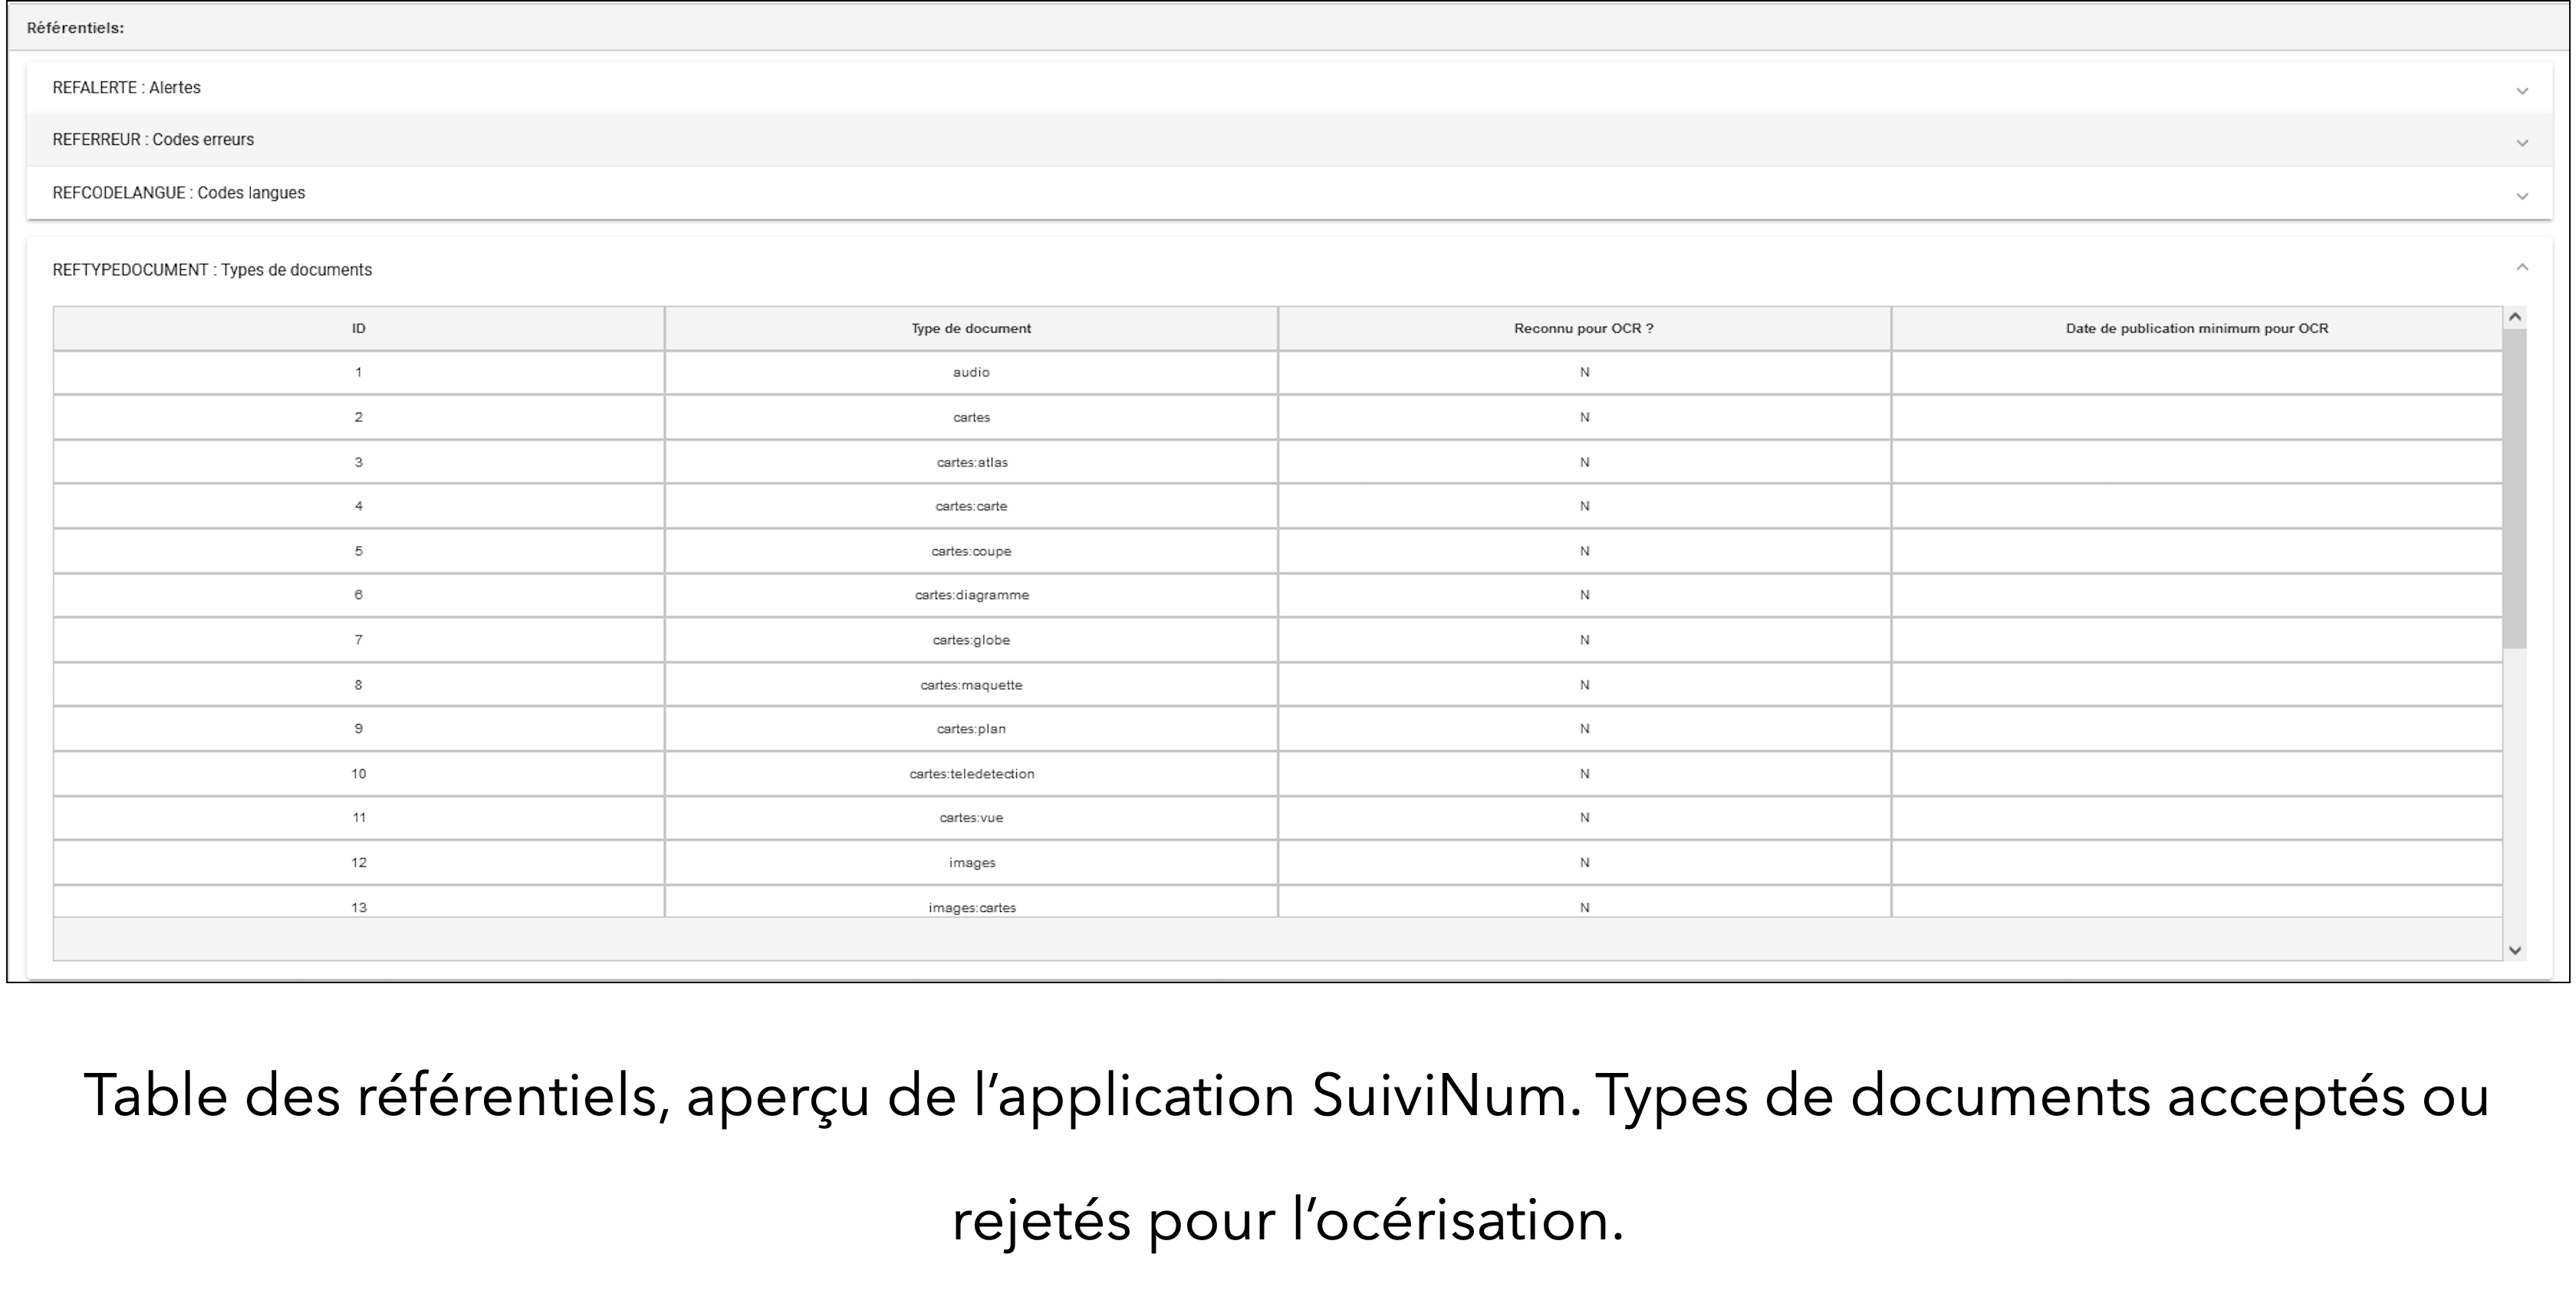
\includegraphics[width=0.8\textwidth]{images/ref_table_a.png}
		\caption{Table des référentiels, aperçu de l’application SuiviNum. Types de documents acceptés ou rejetés pour l’océrisation. }
		\label{fig:monimage}
	\end{figure}
	
	\begin{figure}[h!]
		\centering
		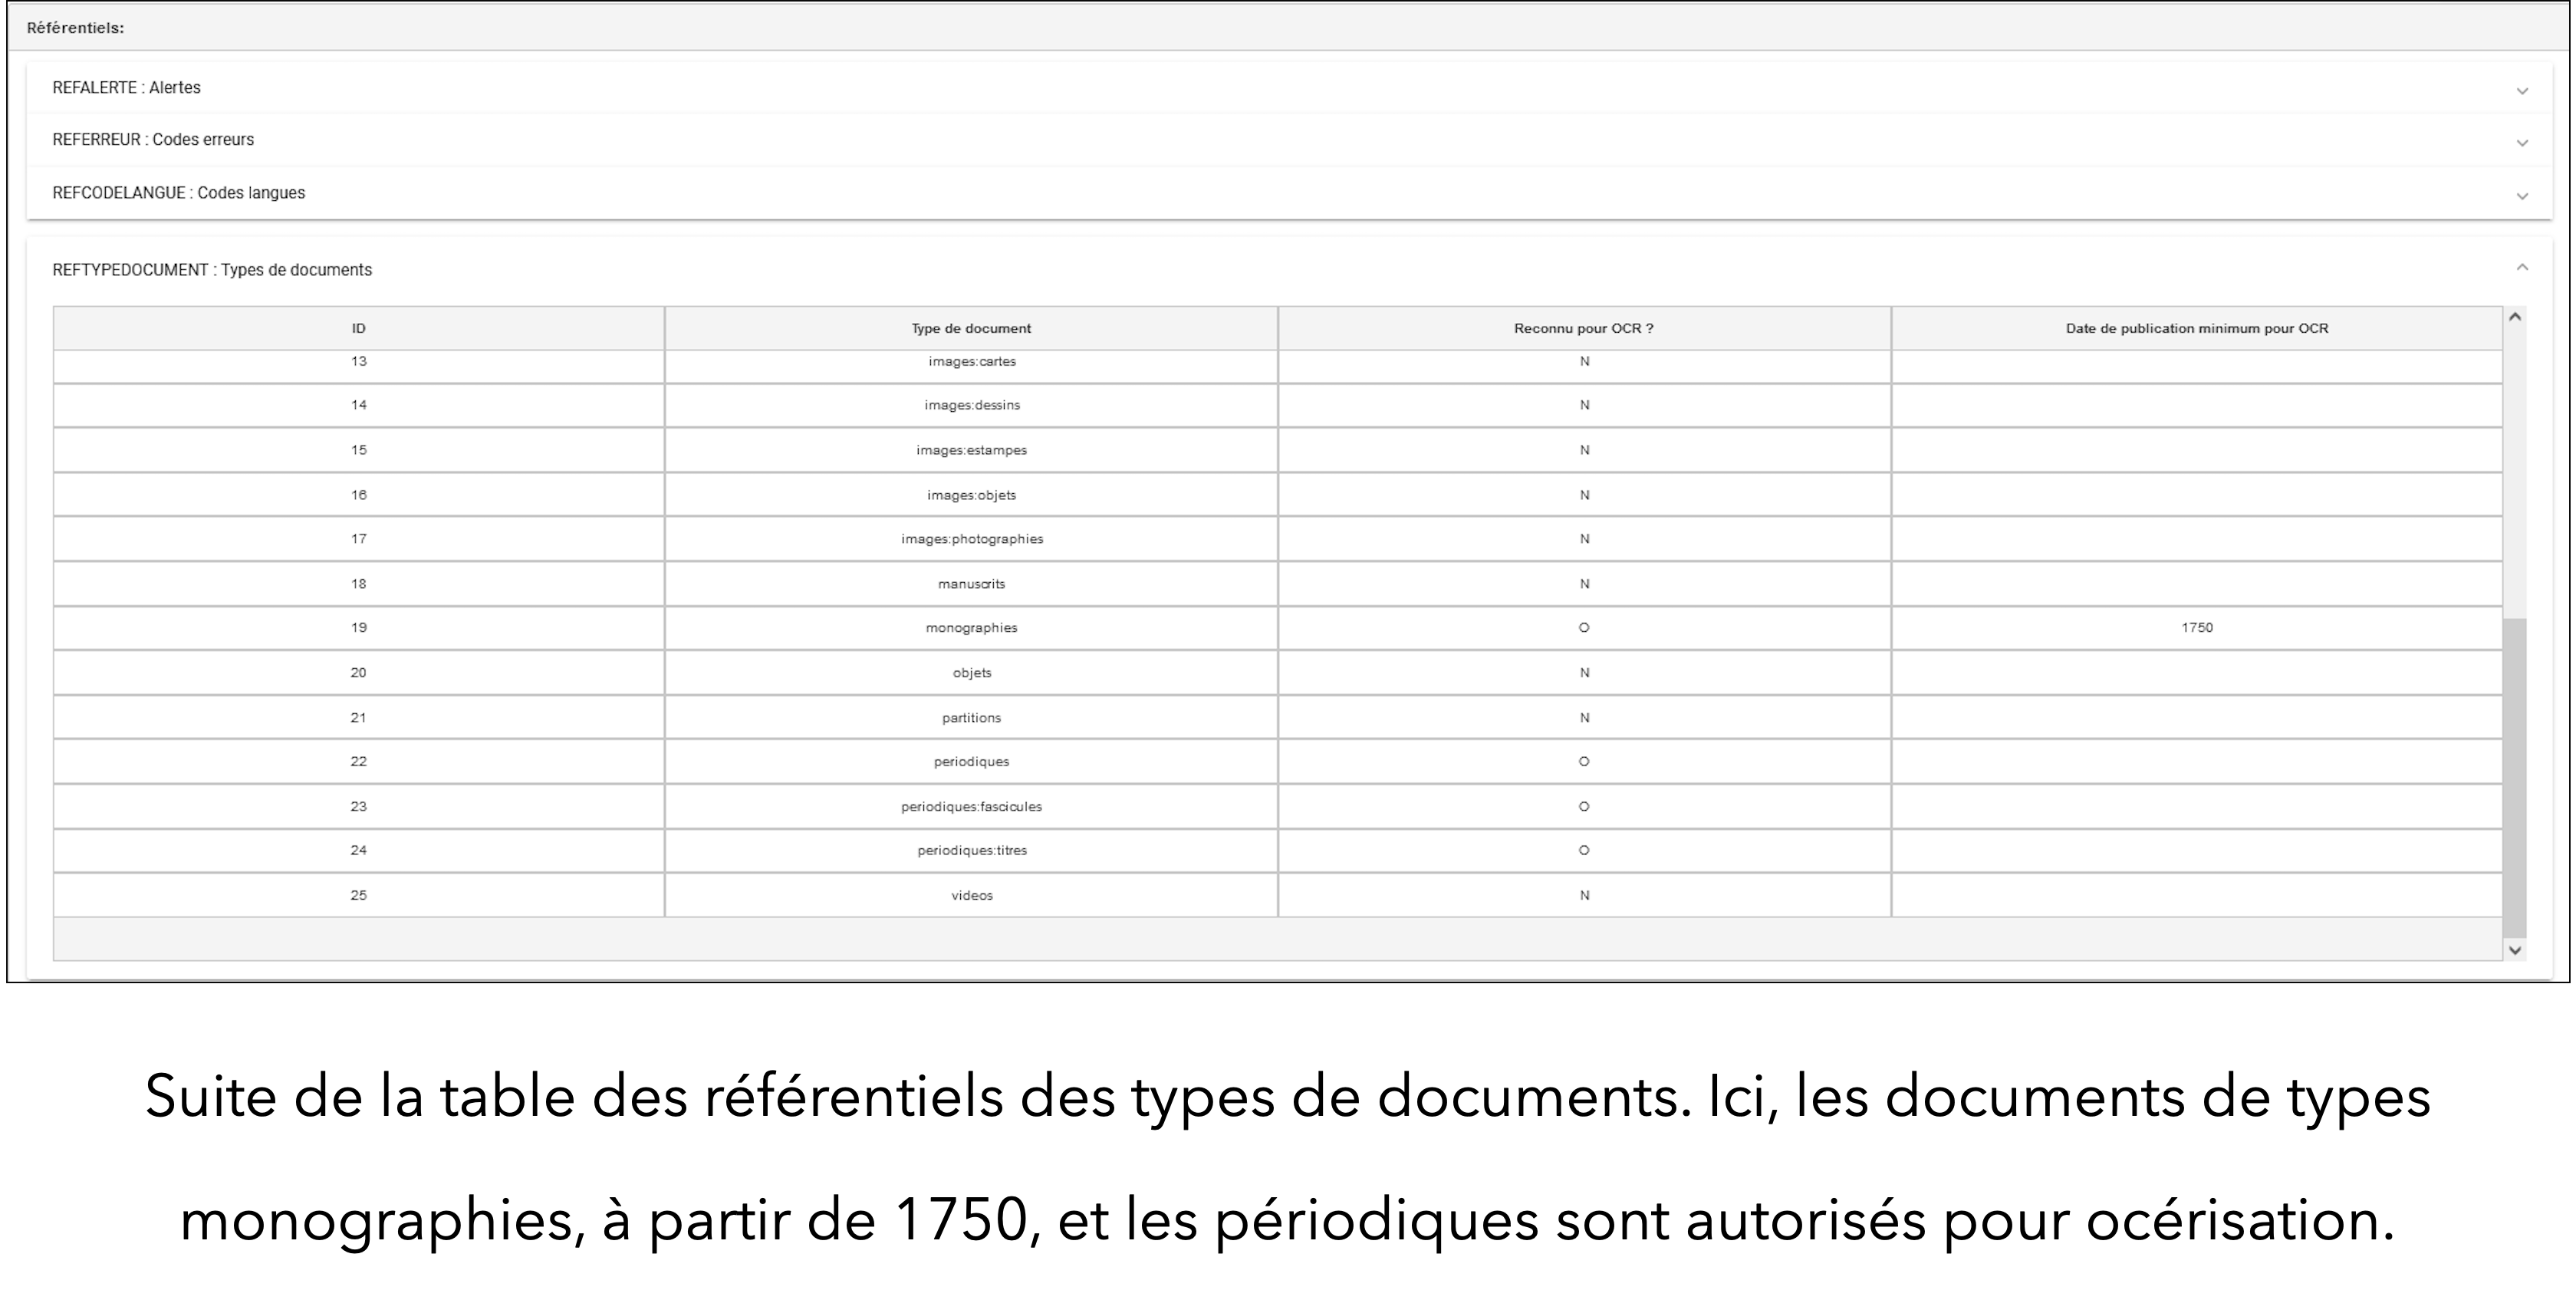
\includegraphics[width=0.8\textwidth]{images/ref_table_b.png}
		\caption{Suite de la table des référentiels des types de documents. Ici, les documents de types monographies, à partir de 1750, et les périodiques sont autorisés pour océrisation.}
		\label{fig:monimage}
	\end{figure}
	
	Il en est de même avec le code langue. Le moteur OCR doit connaître la langue du document pour proposer une océrisation, car il ne détermine pas de façon autonome la langue d’un document. Pour cela, on interroge l’entrepôt OAI de la BnF afin d’obtenir le code langue du document. En interrogeant cet entrepôt, les données récupérées permettent d'identifier si le document est en français, latin, allemand ou occitan, par exemple\footcite{de_lavenne_de_la_montoise_oai-pmh_2020}. Certains documents peuvent avoir plusieurs langues enregistrées dans la métadonnée code langue. Lorsque la langue n’est pas reconnue, le document passe à l’état « abandonné » dans la table, signifiant qu'il y a eu une demande d’océrisation pour ce document mais qui ne sera jamais reprise car le code langue ne concorde pas avec les exigences du moteur OCR. Cela se produit notamment lorsque le document est multilingue.
	
	Concernant le moteur OCR, l’établissement a acquis une licence pour numériser l’équivalent de 20 millions de pages, équivalent format A4 avec le moteur ABBYY, que nous présenterons plus en détail ultérieurement. Ce moteur prend en charge de nombreuses langues comme le français, le grec, le tatar, ou encore l’azerbaïdjanais. Bien que la prise en charge de l’ancien français soit prévue, elle n'est pas encore fonctionnelle pour le moment.  
	\\
	
	La Bibliothèque nationale de France utilise SPAR (Système de Préservation et d'Archivage Réparti) comme pierre angulaire de sa stratégie de conservation numérique\footcite{bermes_approche_2010}. Lancé en 2010, SPAR est bien plus qu'un simple outil de stockage ; c'est un dispositif complexe visant à pérenniser l'information numérique. Les missions principales de la BnF sont :
	\begin{enumerate}
		\item La conservation du patrimoine
		\item La diffusion des connaissances
	\end{enumerate}
	
	SPAR s'inscrit dans la mission de conservation, avec l'ambitieux objectif de préserver les documents numériques sur le très long terme. Son rôle va au-delà de l'archivage sécurisé, Il assure la lisibilité à long terme des documents, malgré l'évolution des technologies. Et il maintient la compréhensibilité et la réutilisabilité de l'information, indépendamment des changements d'environnement technique et humain.
	\\
	
	Face aux défis de la dégradation numérique et de l'obsolescence technologique, SPAR adopte une approche proactive :
	\begin{itemize}
		\item Veille technologique constante
		\item Migrations préventives des données
	\end{itemize}
	
	Cette stratégie anticipe les problèmes plutôt que de tenter de réparer des documents déjà endommagés ou devenus illisibles. En constante évolution, SPAR intègre régulièrement de nouvelles collections de la BnF et fonctionnalités, s'adaptant aux besoins croissants de la conservation numérique. 
	
	De plus, le caractère "réparti" de SPAR se manifeste par sa capacité à gérer et stocker de multiples copies des documents sur différents sites géographiques. Cette redondance stratégique vise à minimiser les risques de perte ou de destruction des données, renforçant ainsi la résilience du système de préservation.
	\\
	
	Mais pourquoi parler de SPAR ? Tout simplement car SPAR joue un rôle important dans le processus de numérisation et d'océrisation, se positionnant à la fois en amont et en aval de la chaîne de traitement. En entrée, SPAR fournit les documents numériques initiaux destinés à l'océrisation. Une fois le traitement effectué, le système accueille en sortie les versions OCRisées comme de nouveaux documents. Ces versions enrichies coexistent avec les originaux dans SPAR, formant ainsi une sorte de doublon amélioré. De plus, en sortie de chaîne, le processus se divise en deux volets distincts : d'une part, la préservation à long terme dans SPAR, et d'autre part, la diffusion publique via Gallica.
	\\
	\\
	
	Après avoir examiné le processus de sélection des documents à océriser par la BnF, plongeons au cœur de la chaîne de traitement OCR. La première étape est le passage des documents à la phase de « Demande d'océrisation ». C'est à ce moment que le moteur ABBYY entre en jeu pour effectuer l'OCR sur le document. Avant de nous étendre sur le processus, il est nécessaire de faire un point sur ABBYY.
	
	ABBYY, entreprise américaine leader dans le traitement documentaire, est particulièrement reconnue pour son expertise en OCR. Le « moteur ABBYY » utilisé par la BnF est ABBYY FineReader, un kit de développement permettant aux développeurs de créer des outils capables d'extraire des informations textuelles à partir de diverses sources : documents papier, images, ou même écrans.
	
	FineReader se distingue par ses algorithmes avancés de reconnaissance de texte, offrant une extraction d'informations d'une grande précision tout en préservant la mise en page originale et les éléments structurels du document. Son atout majeur réside dans sa capacité à s'intégrer de manière fluide et transparente dans des workflows, ou flux de travail, automatisés et des solutions de gestion documentaire, le rendant ainsi particulièrement adapté aux environnements de travail complexes et variés, comme la BnF. Cette intégration est facilitée par des API (Application Programming Interface ou Interface de Programmation d'Application) robustes et des outils de développement flexibles. Ces fonctionnalités permettent aux entreprises de personnaliser et d'automatiser leurs processus OCR en fonction de leurs besoins spécifiques, offrant ainsi une solution sur mesure et hautement efficace\footcite{tafti_ocr_2016}.
	\\
	
	Si la BnF a choisit le moteur ABBYY, d’autres moteurs sont aussi sur le marché de l’OCR et peuvent être envisagés par les établissements. 
	
	Du côté open-source, Tesseract\footnote{ Moteur libre développé par Hewlett-Packard dans les années 1980, aujourd’hui maintenu par Google.} s’est révélé performant dans l’extraction de texte, particulièrement pour les tableaux. Cependant, il a montré des limitations lorsqu’il s’agissait de filtrer les bruits et les bavures sur des documents plus anciens, comme les journaux du XIXe siècle. De plus, bien que Tesseract soit une alternative gratuite intéressante, le suivi technique derrière n’est pas assuré comme peut le faire par exemple ABBYY au travers d’un support technique. Autre logiciel intéressant : Adobe Acrobat Pro. Bien qu’il soit largement utilisé pour l’édition et la gestion de PDF, ses performances en matière d’OCR ont été jugées inférieures à celles d’ABBYY et de Tesseract, en particulier pour les documents historiques. Les erreurs fréquentes d’Adobe, telles que l’insertion d’espaces supplémentaires au milieu des mots ou la fusion incorrecte de mots, ont un impact significatif sur la précision des recherches textuelles dans les bases de données numérisées, rendant son utilisation moins adaptée pour des projets d’archives complexes\footcite{olson_digitization_2021}.
	
	Ainsi, bien que chaque logiciel présente des avantages spécifiques selon le contexte d’utilisation, ABBYY FineReader se distingue comme l’outil le plus complet et efficace pour les projets de numérisation exigeant une haute précision et une gestion complexe de la mise en page, tel que le traitement des documents à la BnF.
	\\
	
	Pour lancer le processus d'océrisation des documents, les équipes de la BnF utilisent une application nommée SchedulingTool. Cette application, que l'on pourrait qualifier de « tuyauterie », fonctionne comme un lanceur permettant d'initier des tâches de façon périodique. Par exemple, elle peut traiter un nombre défini de documents toutes les x secondes, minutes ou jours. À la BnF, les documents sont traités à intervalles réguliers de x minutes. Cette approche permet une gestion efficace de l'espace de stockage. Si un paquet de données occupe 50 mégaoctets et qu'un million de paquets similaires sont en attente, l'espace total requis atteindrait 50 pétaoctets, soit 50 000 téraoctets. Or, les capacités de stockage de la BnF, bien que considérables, ne sont pas illimitées. De plus, cette gestion minutieuse permet d'optimiser l'utilisation des ressources informatiques, assurant ainsi un flux de traitement continu et efficace. 
	
	Mais concrètement, si nous changeons d’échelle, que voit-on ? Tout ceci est visible via l’application SuiviNum, dont nous détailleront le fonctionnement par la suite. Le processus détaillé se déroule comme suit :
	\begin{enumerate}
		\item Prise en compte de la demande d'océrisation
		\item Fabrication du paquet de données
		\item Récupération des images via les systèmes SPAR 
		\item Traitement OCR proprement dit
	\end{enumerate}
	Le cœur du système est le GenOCR Manager, qui gère la distribution des tâches aux workers. Ce manager récupère les documents, prend les images, et les envoie aux workers pour traitement. La BnF dispose de 4 serveurs dédiés, chacun avec 32 threads\footnote{un « fil d’exécution », en français, est une séquence d’instructions que l’OS - système d’exploitation - peut gérer indépendamment. Cela permet à un programme de pouvoir exécuter plusieurs tâches en simultané. Ici, cela signifie donc que chaque serveur peut exécuter 32 tâches de traitement simultanément. }, qui tournent continuellement pour optimiser le processus. Ces workers traitent les images en parallèle, page par page, sans notion de document complet. C'est le manager qui reconstitue le document une fois toutes les pages traitées. 
	
	Petit point sur les workers : ce que l'on appelle un « worker » est un composant logiciel spécialisé qui exécute des tâches spécifiques. À la BnF, il s'agit d'un programme écrit en JAVA, un langage de programmation. Ce programme permet de gérer les océrisations page par page, traitant chaque image individuellement. Les workers sont supervisés par un « manager », lui aussi un composant logiciel, qui joue un rôle crucial dans la coordination et la supervision de l'ensemble du processus. Le manager remplit plusieurs fonctions essentielles. Il est responsable de la distribution des tâches, assignant les pages à océriser aux différents workers disponibles. Il surveille en temps réel la progression de chaque tâche attribuée et coordonne l'ensemble pour s'assurer que le système fonctionne de manière fluide et efficace. De plus, le manager veille à ce que les workers puissent récupérer les nouvelles tâches à partir d'une file d'attente centralisée. Il supervise également la gestion des erreurs éventuelles par les workers, assurant ainsi la robustesse du système. Cette architecture permet une parallélisation efficace du traitement, optimisant ainsi les performances globales du système d'océrisation de la BnF. Le manager agit comme un chef d'orchestre, s'assurant que chaque worker joue sa partition au bon moment, tout en maintenant la cohérence de l'ensemble du processus.
	
	Cette approche permet une gestion efficace de l'espace de stockage et des ressources informatiques. Pour une efficacité optimale, le système maintient entre 200 et 400 pages en traitement simultané. Cette gestion minutieuse permet d'optimiser l'utilisation des ressources informatiques, assurant ainsi un flux de traitement continu et efficace. Un point intéressant à noter est la flexibilité du système. En théorie, si la BnF décidait de changer de moteur OCR, passant par exemple d'ABBYY à un moteur open source comme Tesseract, cela serait possible en modifiant simplement les workers. Cependant, ABBYY reste privilégié pour ses performances, notamment en matière de pré-traitement des images.
	
	Une fois l'OCR terminé, le document suit le processus normal de la chaîne d'entrée\footnote{Cf. Annexe, Schéma \ref*{fig:schemnumbnf}} de la BnF. Tout ce processus est visible via l'application SuiviNum, que nous détaillerons par la suite.
	La chaîne d'entrée est un processus qui reçoit les documents numérisés, qu'ils proviennent d'un prestataire externe ou interne comme nous l'avons vu précédemment. Il s'agit d'un paquet contenant des images et des fichiers de métadonnées (master). Cette chaîne effectue des vérifications et des contrôles sur les métadonnées afin de s'assurer que tout soit en ordre et que les références concordent avec la notice du catalogue de la BnF. Un contrôle est également réalisé sur les images pour vérifier leurs dimensions et s'assurer que le document n'est pas corrompu. Ensuite, le catalogue est sollicité afin de mettre à jour la notice du document et pour signaler sa numérisation. Le document sera alors envoyé sur Gallica pour la diffusion et sur SPAR pour la conservation.
	
	Cette chaîne d'entrée, que nous avons déjà plus ou moins évoquée, mérite d'être explicitée car un document océrisé (ou « traitement complémentaire »)  repasse par le même chemin qu'un document numérisé pour la première fois (une « primo-livraison »). C'est comme si on traitait un nouveau document à part entière. Cette approche assure une cohérence dans le traitement de tous les documents, qu'ils soient nouvellement numérisés ou qu'ils aient bénéficié d'une océrisation ultérieure.
	
	La différence entre les primo-livraisons et les traitements complémentaires, comme l’OCR, réside dans la présence de nouveaux fichiers : les ALTO. Le XML ALTO, acronyme d’Analyzed Layout and Text Object, est un format XML émergent au sein des communautés de bibliothèques numériques, conçu pour représenter les résultats de la reconnaissance optique de caractères (OCR). Ce format est utilisé pour décrire la disposition physique et le contenu textuel des pages numérisées. Dans le cadre de l’OCR à la BnF, les fichiers ALTO jouent un rôle crucial en structurant les informations extraites par le processus d’océrisation. Ces fichiers ne se contentent pas de conserver le texte brut, mais incluent également des données précieuses telles que les positions exactes du texte sur la page, les différents styles typographiques utilisés, ainsi que l’emplacement des images. Cette approche permet de préserver fidèlement la mise en page originale des documents\footcite{belaid_xml_2007}.
	
	De plus, l'OCR interne ajoute une difficulté supplémentaire : la création d'un nouveau manifeste qui renseigne l'océrisation. Comme nous l'avons déjà mentionné, le fichier d'un document numérisé se compose des images et d'un fichier de métadonnées, appelé manifeste. Dans le cas de l'OCR, on ajoute non seulement les fichiers ALTO à ce dossier, mais on doit également créer un nouveau manifeste qui indique qu'une océrisation a été effectuée sur le document, ce nouveau manifeste venant compléter les informations du document initial. À la suite de cela, LIVATEL, un nouveau batch\footnote{ Ensemble de données ou de tâches regroupées pour être traitées ensemble, ce qui permet d’améliorer l’efficacité et la stabilité du processus de traitement.}, va chercher les paquets océrisés qui se trouvent sur un espace de stockage puis va les livrer à la chaîne d'entrée. Pour bien illustrer, il faut imaginer deux espaces bien distincts : d'un côté l'espace de production, où l'on va ajouter les ALTOs au fur et à mesure de leur création, et de l'autre un espace de livraison de paquets, la « PEF », pour Plateforme d’Échange de Fichiers, où la chaîne d'entrée va scruter les paquets qui ont été livrés afin de les intégrer dans le processus d'entrée. Les documents sont distribués dans des dossiers de prestations (un dossier par prestation) et les documents océrisés sont acheminés vers les prestations 560 à 564. Pour comprendre, le 560 représente le courant, le 561 représente le rétrospectif, le 562 représente l'espace ESCO (les partenaires livrant des images), 563 est pour les ateliers internes de la BnF et le 564 pour l'OCR à la demande (on peut prendre en compte le 565 urgences mais il n'a jamais été activé).
	
	Point rapide sur les dossiers de prestation : Pourquoi avoir des dossiers séparés ? Tout simplement car il n'y a pas que de l'OCR dans les dossiers,  ces derniers contiennent tous les prestataires de la BnF. Et ces prestataires font exactement la même chose que LIVATEL, après numérisation, ils envoient via un client FTP, File Transfert Protocol ou Protocole de Transfert de Fichiers\footnote{ Protocole permettant de pouvoir transférer des fichiers entre un ordinateur local et un serveur distant via le protocole FTP. Il offre une interface pour naviguer dans les répertoires du serveur, télécharger des fichiers depuis le serveur vers l'ordinateur local (download), et envoyer des fichiers depuis l'ordinateur local vers le serveur (upload). Les clients FTP sont couramment utilisés pour gérer le contenu de sites web, partager des fichiers volumineux, ou synchroniser des données entre différents systèmes.}, des paquets numérisés afin qu'ils puissent entrer dans la chaîne. 
	\\
	
	Avant de rentrer dans la présentation de SuiviNum, il est important d’expliquer comment fonctionne la chaîne d’entrée. 
	La chaîne d'entrée est un processus qui reçoit les documents numérisés par le prestataire, comprenant des images et des fichiers de métadonnées. On vérifie alors que les métadonnées sont correctes et que les références à la notice du catalogue sont exactes. Les documents sont ensuite envoyés, dans un premier temps, vers la préservation avec SPAR, puis vers la diffusion afin qu'ils soient disponibles sur Gallica. La préservation précède la diffusion afin de pouvoir prendre en compte les éventuels rejets qui peuvent survenir avec SPAR ; le cas échéant, le processus s'arrête à SPAR. La préservation est l'étape la plus importante, car il faut prévenir les problèmes potentiels (crashes informatiques, malveillance, incendie, etc.), d'où l'utilisation de SPAR avant la diffusion sur Gallica.
	\\
	
	Un point central dans ce processus est le suivi de la chaîne d'entrée. Pour assurer la supervision, une table de suivi a été mise en place, offrant à tous les intervenants une vue d'ensemble sur l'état d'avancement des documents. Cette table indique avec précision à quelle étape du processus chaque document se trouve et dans quel état il est. L'application SuiviNum joue ici un rôle clef en proposant une interface graphique intuitive qui donne un aperçu clair et détaillé de ce qui se passe au cœur de la chaîne. SuiviNum permet de suivre toutes les chaînes d'entrée de la BnF, pas uniquement l'OCR. Cette table comporte des colonnes essentielles :
	\begin{itemize}
		\item Une colonne pour les documents en attente.
		\item Les colonnes d'état : Indiquant si le document est en demande d'océrisation ou en cours d’océrisation.
		\item Les colonnes d'erreurs : Signalant s'il y a eu une erreur fonctionnelle ou technique, ou si les documents ont été abandonnés et sont à relancer.
	\end{itemize}
	
	\begin{figure}[h!]
		\centering
		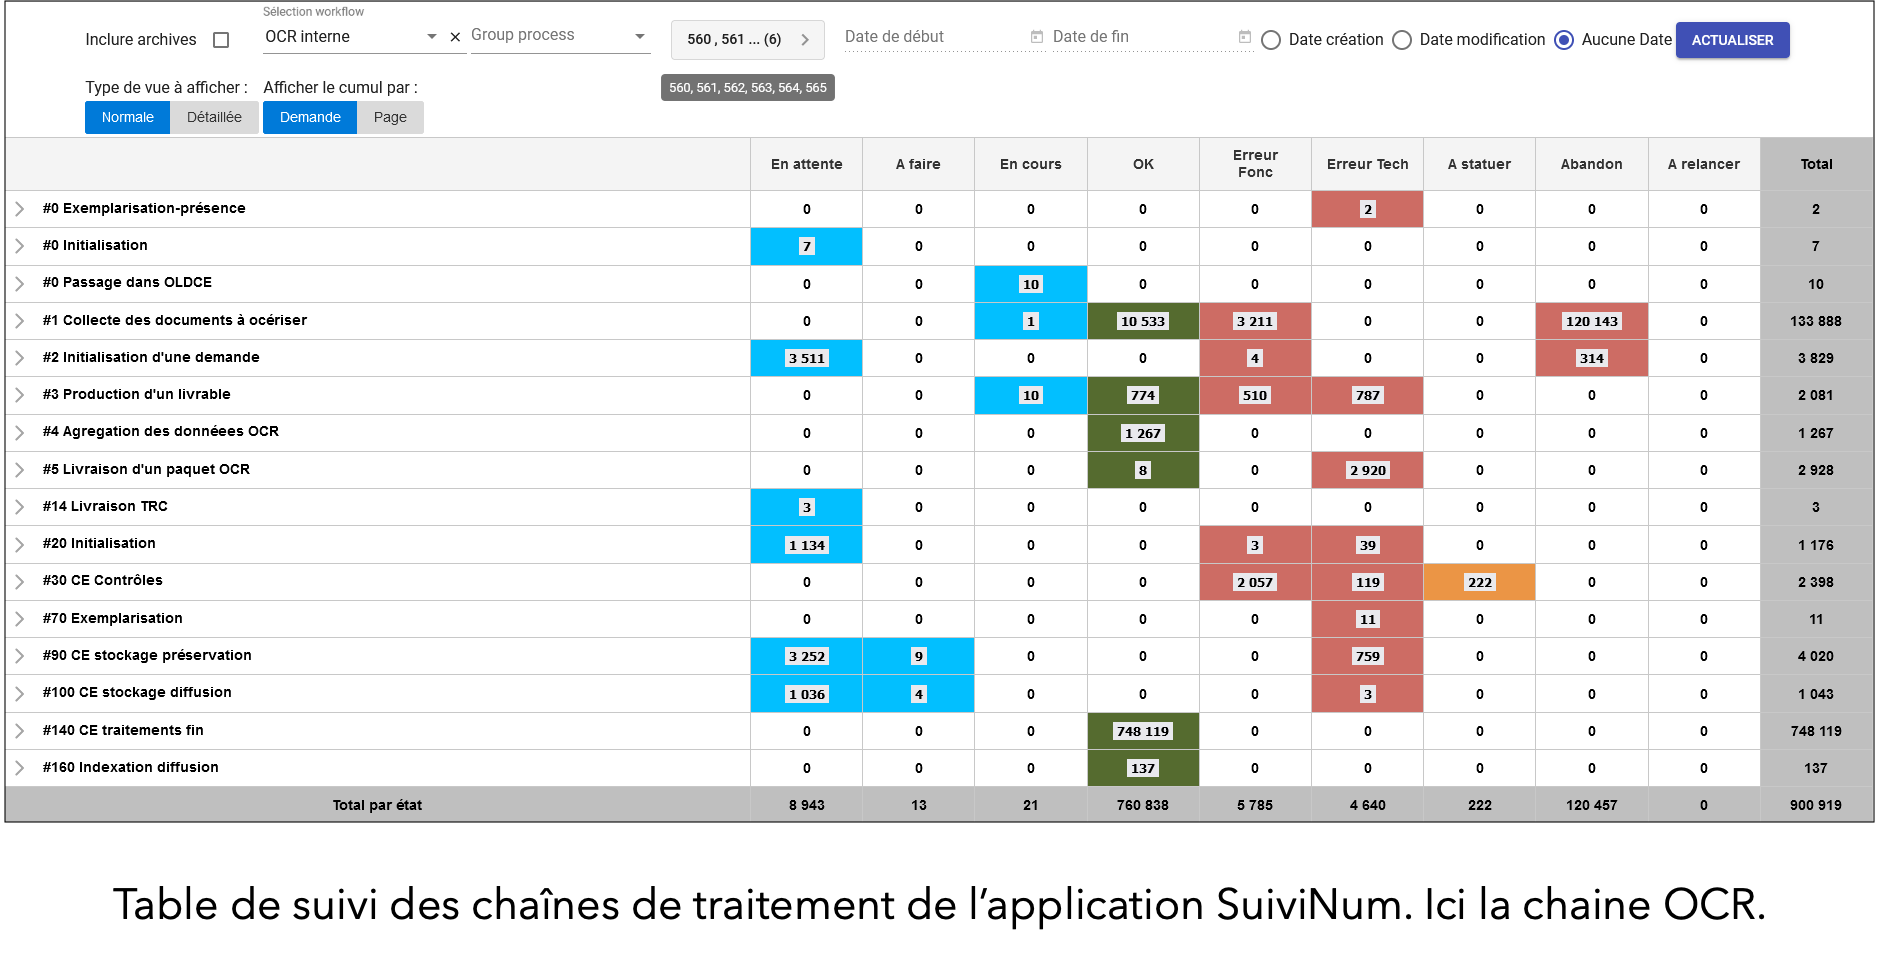
\includegraphics[width=0.8\textwidth]{images/suivi_num.png}
		\caption{Table de suivi des chaînes de traitement de l’application SuiviNum. Ici la chaine OCR. }
		\label{fig:monimage}
	\end{figure}
	
	La table se met à jour en continu pour fournir un suivi en temps réel des flux grâce aux différentes applications vues jusqu'ici. Chaque application informe de l'avancée ou d'une erreur d'un document et le renseigne dans SuiviNum. En cas de plantage d'application ou d'erreur d'accès à un fichier, elle place le document en état 7 « KO Technique ». L'équipe fonctionnelle, le BEA, pour Bureau Études et accompagnement, peut alors le relancer.
	
	Concernant les erreurs, nous avons identifié deux types principaux : l'erreur fonctionnelle et l'erreur technique. La première provient de la prestation elle-même, tandis que la seconde est une erreur interne pouvant avoir diverses origines : une donnée mal renseignée, un « plantage » informatique, etc. Les erreurs fréquentes sont souvent liées à un code langue incorrect, comme mentionné précédemment. Un autre problème rencontré est la « fausse erreur », une erreur fonctionnelle qui n'en est pas vraiment une, souvent à cause de crash serveurs. 
	
	SuiviNum s'avère également être un outil précieux pour les différents départements de la BnF. Comme évoqué plus haut, il permet d'avoir une visualisation graphique en temps réel des flux, offrant ainsi la possibilité d'obtenir des chiffres sur ce qui est réalisé et ce qui reste à faire. Par exemple, on peut suivre le nombre de pages, équivalent A4, numérisées au cours de l'année\footnote{Cf. Annexes, Figure \ref{fig:statsuivinum}}, ou encore obtenir des statistiques sur les x derniers jours par type de documents\footnote{Cf. Annexes, Figure \ref{fig:compteurocr}}. Ces informations permettent aux chefs de projets d'avoir une idée précise de l'avancement des différentes prestations dont ils ont la charge. C'est également un outil de reporting indispensable pour l'équipe de numérisation de la BnF.
	\\
	
	Cependant, cette technologie, outre ses avantages considérables pour une institution comme la BnF, apporte son lot de défis, notamment en termes de gestion des volumes de données, comme l'illustre l'exploration de la chaîne de traitement OCR.
	
	Le premier défi est d'ordre physique. Les institutions patrimoniales comme la BnF sont confrontées depuis longtemps au stockage d'objets matériels tels que les livres et les manuscrits. Aujourd'hui, elles doivent également gérer le stockage de l'immatériel : données, fichiers et images numériques. Cette nouvelle réalité nécessite la mise en place de data centers, véritables centres névralgiques où sont stockés les paquets OCR, les œuvres numérisées et les données associées. Ces installations requièrent un espace conséquent pour accueillir des racks (ou baies), sortes d'armoires renfermant les appareils de stockage et de réseau. Disposer d'une capacité de stockage de l'ordre du pétaoctet (PB) ou de l'exaoctet (EB) , sachant qu'un EB équivaut à 1000 PB, implique des investissements importants en termes d'espace et d'infrastructure. S'ajoutent à cela les coûts financiers liés à l'entretien des serveurs, à la gestion des racks et à leur consommation énergétique.
	
	Le second défi concerne la gestion des flux de données. La capacité de stockage de la BnF, bien que considérable, n'est pas illimitée. Il est donc crucial d'optimiser la gestion des flux, tant pour la chaîne de traitement OCR que pour la chaîne d'entrée des documents. L'objectif est de maintenir un fonctionnement automatique et continu des chaînes, en s'assurant qu'elles aient toujours des éléments à traiter. Dans ce contexte, l'OCR joue un rôle de variable d'ajustement. La production quotidienne d'OCR est adaptée en fonction du volume de nouvelles livraisons : elle est augmentée lorsque les entrées sont faibles et réduite en période de forte affluence de nouveaux documents.
	
	Un problème majeur a récemment mis en lumière la complexité de cette gestion des flux. En effet, un même document numérique passe d'abord par la chaîne d'entrée pour ses images, puis une seconde fois pour l'OCR interne. Cette double entrée a provoqué une saturation de la chaîne d'entrée, bloquant tout le circuit d'océrisation interne pendant plus d'un an. 
	
	Pour donner une idée de l'ampleur de l'infrastructure nécessaire, la chaîne d'entrée utilise à elle seule 22 serveurs dédiés. Le système SPAR fonctionne sur environ 50 machines virtuelles (VM). L'OCR, quant à lui, mobilise 4 machines dédiées uniquement au calcul. Actuellement, SPAR gère un volume de stockage de 6 pétaoctets, multiplié par 4 car les données sont stockées sur deux zones différentes pour des raisons de sécurité et de redondance.
	
	Cette situation illustre parfaitement les défis techniques et logistiques auxquels font face les grandes institutions culturelles à l'ère du numérique. La gestion de tels volumes de données requiert non seulement des infrastructures conséquentes, mais aussi une planification minutieuse et une capacité d'adaptation constante face aux imprévus.
	
	\subsection{ Analyse et fonctionnement d’une chaîne HTR}
	
	Après avoir détaillé la chaîne de traitement OCR\footnote{Cf. Annexes, Schéma \ref*{fig:schemocrbnf}} de la Bibliothèque nationale de France, il est pertinent d’examiner la mise en place d’une chaîne dédiée à la reconnaissance d’écritures manuscrites, communément appelée HTR. À l’heure actuelle, la BnF ne dispose pas d’une infrastructure interne pour traiter les documents manuscrits via HTR. C’est pourquoi, dans le cadre d’un stage à la BnF, une chaîne de traitement HTR fonctionnelle a été mise en place à une échelle réduite. Ce projet visait à évaluer l’efficacité des modèles HTR génériques actuellement disponibles pour le traitement de masse, en se concentrant sur des documents issus de différentes époques, rédigés par des mains variées, mais dans une langue commune : le français.
	
	Avant d’explorer plus en détail les spécificités techniques de la chaîne HTR, il est crucial de comprendre le contexte et les perspectives de l’HTR par rapport à l’OCR. L’OCR est une technologie bien établie qui a révolutionné la numérisation et l’exploitation des documents imprimés. Cette technologie permet de convertir des textes imprimés en données numériques, facilitant ainsi leur recherche, leur indexation et leur analyse. Cependant, malgré ses avancées significatives, l’OCR montre ses limites face aux documents manuscrits. En effet, les caractères manuscrits sont souvent irréguliers, variant en fonction du scripteur, du support et de l’époque, rendant l’identification par l’OCR souvent imprécise ou inefficace. 
	
	C’est dans ce contexte que l’HTR se positionne comme une technologie indispensable, en particulier pour les institutions patrimoniales telles que la BnF, qui gèrent d’importantes collections de manuscrits. L’HTR est spécifiquement conçu pour reconnaître et transcrire des écritures manuscrites, y compris celles qui sont cursives et présentent une grande variabilité graphique. Alors que l’OCR se focalise principalement sur les textes imprimés, l’HTR permet de relever le défi de la diversité des écritures manuscrites, apportant ainsi une solution à un problème longtemps considéré comme insurmontable. Grâce à des modèles d’apprentissage profond et à des techniques d’intelligence artificielle avancées, l’HTR peut identifier et transcrire des caractères manuscrits avec une précision accrue, même dans des conditions difficiles telles que des documents anciens ou endommagés\footcite{cretin_transcription_2023}.
	\\
	
	Tout comme pour la chaîne OCR, il est nécessaire de sélectionner les documents à traiter pour obtenir les meilleurs résultats possibles. Pour ce faire, les documents doivent être déjà numérisés et présents sur Gallica. Comme nous l’avons vu plus tôt, la bibliothèque numérique de la BnF dispose, après interrogation de l’entrepôt OAI de la BnF, de 203 252 documents classés comme « manuscrits ». Pour pouvoir examiner la spécificité des manuscrits,  l’entrepôt nous renvoie des fichiers en format XML qui contiennent les métadonnées de chaque document numérisé à la BnF, qu'ils soient internes ou fassent partie de la collection d’un partenaire. L’entrepôt OAI conserve des métadonnées au format Dublin Core, un format descriptif ayant pour objectif de fournir un ensemble standardisé d’éléments descriptifs pour faciliter la découverte et l’accès aux ressources à travers différentes communautés et divers formats descriptifs spécifiques à chaque domaine, tout en conservant une structure claire. Le Dublin Core se compose de 15 éléments facultatifs et répétables :
	\begin{itemize}
		\item Description du contenu : Title, Subject, Description, Source, Language, Relation, Coverage
		\item Propriété intellectuelle : Creator, Contributor, Publisher, Rights
		\item Caractéristiques de l'instance : Date, Type, Format, Identifier
	\end{itemize}
	
	La BnF utilise le format non qualifié de Dublin Core pour plusieurs raisons. Tout d'abord, il permet de gérer sa collection de documents numérisés dans Gallica et d'accroître leur visibilité. De plus, ce format facilite l'interopérabilité, permettant à d'autres institutions, comme des musées ou des archives, de référencer les données de la BnF de manière simple et efficace. Il est important de noter que le Dublin Core ne remplace pas les formats bibliographiques traditionnels comme INTERMARC ou EAD, mais offre un moyen standardisé et adaptable de partager des informations\footcite{goos_dublin_2002}.
	
	Une fois les fiches XML des manuscrits extraites et regroupées, une vérification des métadonnées est nécessaire pour optimiser le traitement des documents. Pour cela, il suffit d'examiner la fiche XML. Une fiche XML d’un document numérisé de la BnF se divise en différentes zones, et celles qui nous intéressent aujourd’hui sont les balises situées entre les balises <metadata>, contenant les données au format Dublin Core, comme <dc:title> ou <dc:description>, et la fin du fichier, où les données sont renseignées par des balises uniques, comme <source>, <typedoc> ou <title>\footnote{Cf. Annexes, Figure \ref{fig:fichexmloai}}. Il est important de mettre en évidence les doublons ou les données lacunaires et de conserver uniquement la donnée au format Dublin Core en cas de répétition ou de données manquantes dans les balises uniques.
	\\
	
	Une fois cette étape achevée, un tri s'avère nécessaire pour obtenir une vue d'ensemble du corpus et mettre en évidence la diversité des manuscrits présents dans la collection de la BnF. Certaines métadonnées sont cruciales pour constituer un corpus pertinent pour le traitement HTR et pour former des sous-corpus documentaires, permettant ainsi une analyse précise des documents disponibles. Cette classification est rendue possible grâce aux métadonnées contenues dans les balises <dc:language>, <dc:date>, <dc:description> et <dc:format>. Un script Python, un langage de programmation de haut niveau\footnote{ Langage de programmation qui abstrait les détails complexes du matériel informatique, facilitant ainsi la lecture, l'écriture et la maintenance du code par les humains.}, est utilisé pour examiner ces fiches et en extraire les données pertinentes. Les informations extraites sont ensuite enregistrées dans un fichier CSV (Comma-Separated Values), un format de fichier texte simple idéal pour stocker des données tabulaires, où chaque ligne représente un enregistrement et les valeurs des champs sont séparées par des virgules. Ce script \footnote{Cf. Annexes, Figure \ref{fig:scriptpythona}} analyse les fichiers XML issus d'un répertoire spécifié afin d'extraire et d'organiser les métadonnées des manuscrits numérisés. Il parcourt méthodiquement chaque fichier XML pour en extraire des informations essentielles telles que la langue, la description, la source, la date et l'identifiant du document. Ces données sont ensuite stockées dans un dictionnaire structuré par langue, facilitant ainsi le regroupement des documents et le décompte du nombre de documents par langue. Le script s'appuie sur les balises Dublin Core pour extraire les métadonnées et intègre une gestion des exceptions pour traiter les éventuelles erreurs lors du traitement des fichiers. Les résultats sont organisés, ouvrant la voie à une analyse approfondie des manuscrits numérisés. Cependant, il est important de faire un point sur les différents problèmes rencontrés avec les métadonnées des manuscrits. 
	\\
	
	Les métadonnées des 203 252 manuscrits sont globalement normalisées, mais certains défis persistent, notamment concernant les dates ou les descriptions fournies par les conservateurs. Ces variations peuvent compliquer l'identification claire et simple des informations. Les balises <date> et <dc:date> illustrent parfaitement cette problématique. En effet, ces métadonnées ne suivent pas un format uniforme pour l'ensemble des documents, et on peut observer une multitude de formats de dates dans les fiches : jj-mm-aaaa, aaaa, aaaa-aaaa, des siècles en chiffres romains, des dates en format littéral (par exemple, "le 13 janvier 1715"), ou encore des années indiquées uniquement par leurs deux premiers chiffres, suggérant ainsi le siècle concerné. Cette diversité de formats nécessite un nettoyage approfondi des données pour obtenir des informations précises et uniformisées, condition sine qua non pour appliquer le modèle HTR approprié aux documents correspondants. Pour relever ce défi, il est impératif de développer un script Python capable d'examiner les balises ciblées, en l'occurrence les dates. Ce script \footnote{Cf. Annexes, Figure \ref{fig:scriptpythonb}} aura pour mission d'extraire et de normaliser les dates contenues dans les fichiers XML des manuscrits, puis de les stocker, associées à des identifiants uniques, dans un fichier JSON\footnote{ JavaScript Object Notation. Format de données textuelles utilisé pour représenter des objets structurés et faciliter l'échange de données.}.
	\\
	
	Une fois le défi de la normalisation des données surmonté, les informations extraites sont intégrées dans une base de données relationnelle SQL\footnote{ Structured Query Language. Langage de programmation utilisé pour gérer et manipuler des bases de données relationnelles.}. Cette étape cruciale permet d'interroger efficacement la base afin de délimiter le corpus qui sera soumis au traitement HTR. La structure de cette base de données comprend diverses tables, chacune représentant des métadonnées jugées pertinentes et essentielles, non seulement pour segmenter le corpus en sous-ensembles cohérents, mais aussi pour appliquer les modèles HTR de manière optimale, et une table concentrant tous les manuscrits de la BnF, avec chaque métadonnée les concernant. Au cœur des tables de métadonnées, on trouve systématiquement deux colonnes principales : la première, intitulée "ARK", contient l'identifiant ARK (Archival Resource Key) attribué par la BnF. Cet identifiant unique et pérenne, assigné aux ressources numériques, garantit leur accessibilité durable et facilite leur gestion. La seconde colonne renferme la valeur spécifique de la métadonnée concernée, qu'il s'agisse de la date, du créateur, de la description, de la langue, du format, ou d'autres attributs pertinents. Concernant la table des manuscrits, on retrouve toutes les colonnes "principales" des autres tables afin de constituer une fiche pour chaque manuscrits.
	
	\begin{figure}[h!]
		\centering
		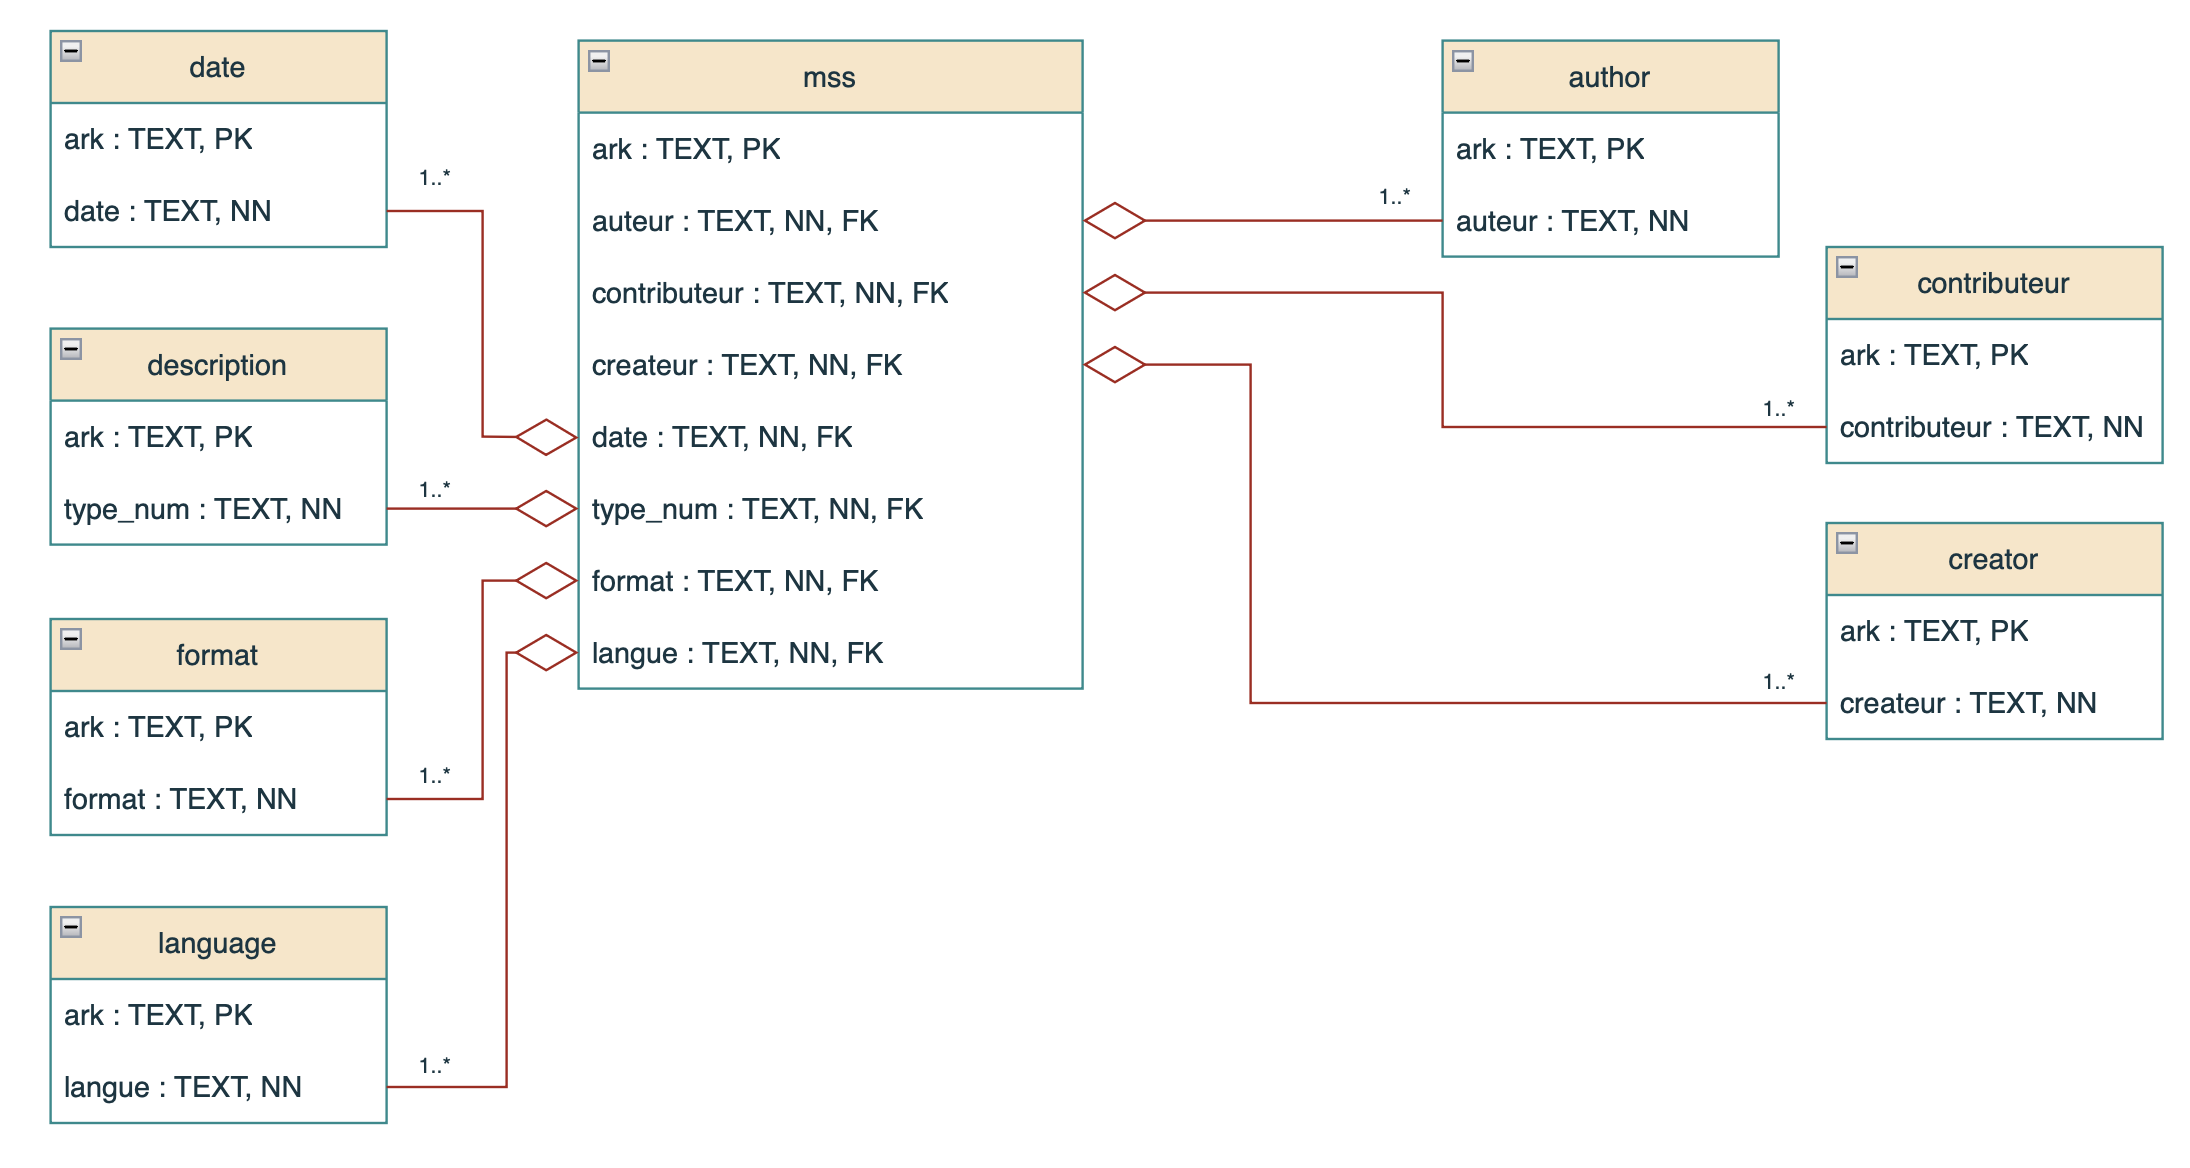
\includegraphics[width=0.8\textwidth]{images/schema_uml_db_mss_bnf.png}
		\caption{Schéma UML de la base de données des manuscrits de la BnF.}
		\label{fig:monimage}
	\end{figure}
	
	Cette structure permet, grâce à des requêtes SQL ciblées, d'extraire une liste précise de documents candidats au traitement HTR. Pour cela, une requête a été conçue pour sélectionner des documents répondant à des critères spécifiques : rédigés en français (à l'exclusion du vieux français), datant de la période allant du XVIIe au XIXe siècle, et issus d'une numérisation directe de documents originaux plutôt que de microfilms. Ce dernier critère vise à garantir une qualité visuelle adéquate, essentielle pour un traitement HTR efficace.  
	\\
	\begin{figure}[h!]
		\centering
		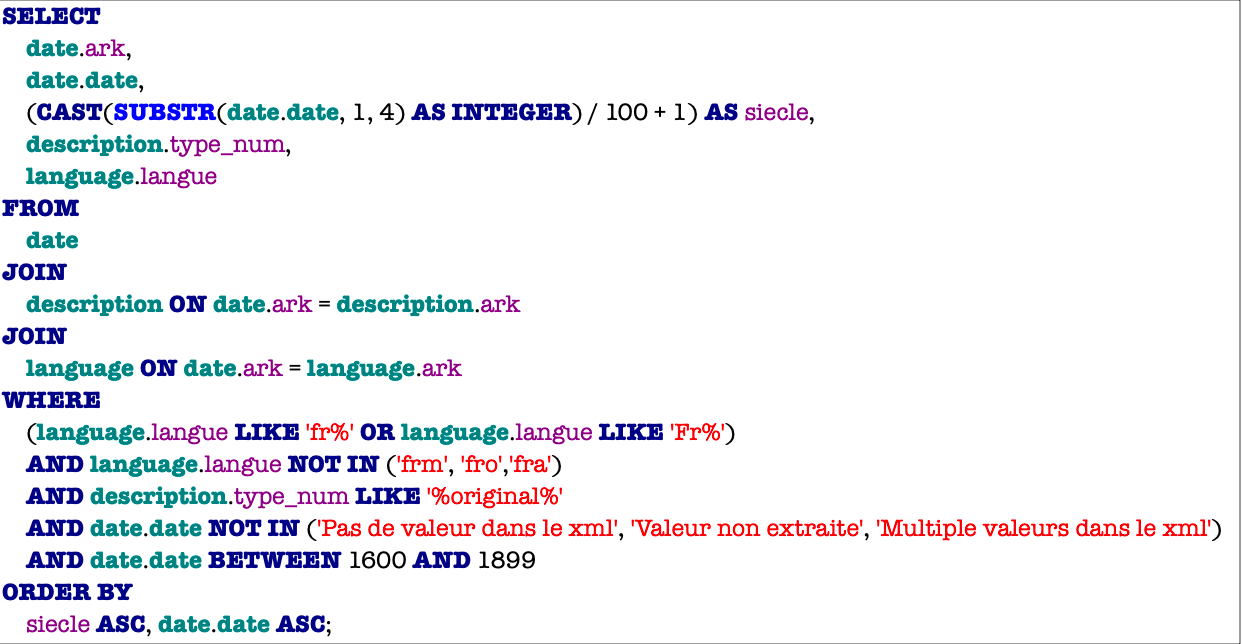
\includegraphics[width=0.8\textwidth]{images/requete_sql.png}
		\caption{Requête en langage SQL afin d’extraire les documents en français, datés entre le XVII et le XIXe siècle issu d’une numérisation à partir d’un original.}
		\label{fig:monimage}
	\end{figure}
	
	Après avoir sélectionné les documents éligibles à un traitement HTR, il est temps d’appeler le moteur et les modèles afin de commencer la reconnaissance de caractères manuscrits. Mais tout d’abord, un point technique sur la définition et la différence entre modèle et moteur. 
	\\
	
	Les modèles ont été évoqués précédemment dans la description de la chaîne, sans pour autant être expliqué.  Un modèle de reconnaissance de texte manuscrit est un algorithme ou un réseau de neurones, une structure computationnelle inspirée du cerveau humain, constituée de nœuds interconnectés (neurones artificiels) qui traitent et transmettent des informations. Ce modèle est spécialement conçu pour reconnaître et transcrire automatiquement du texte manuscrit à partir d’images issues de différents corpus, tels que des documents administratifs, des manuscrits médiévaux, ou des écrits en arabe et en cyrillique. Entraîné sur des données annotées, c’est-à-dire des images de texte manuscrit accompagnées de leurs transcriptions exactes (Corpus Gold), le modèle apprend à généraliser et à transcrire de nouveaux échantillons de texte manuscrit avec une grande précision.
	
	Un aspect important du processus est la correction des données, représentée dans le schéma, figure 3.6\footcite{pinche_images_2022},  par une boucle de rétroaction. Les erreurs détectées dans les prédictions peuvent être corrigées et réintégrées dans le Corpus Gold, permettant ainsi d’améliorer continuellement le modèle HTR.
	\\
	\begin{figure}[H]
		\centering
		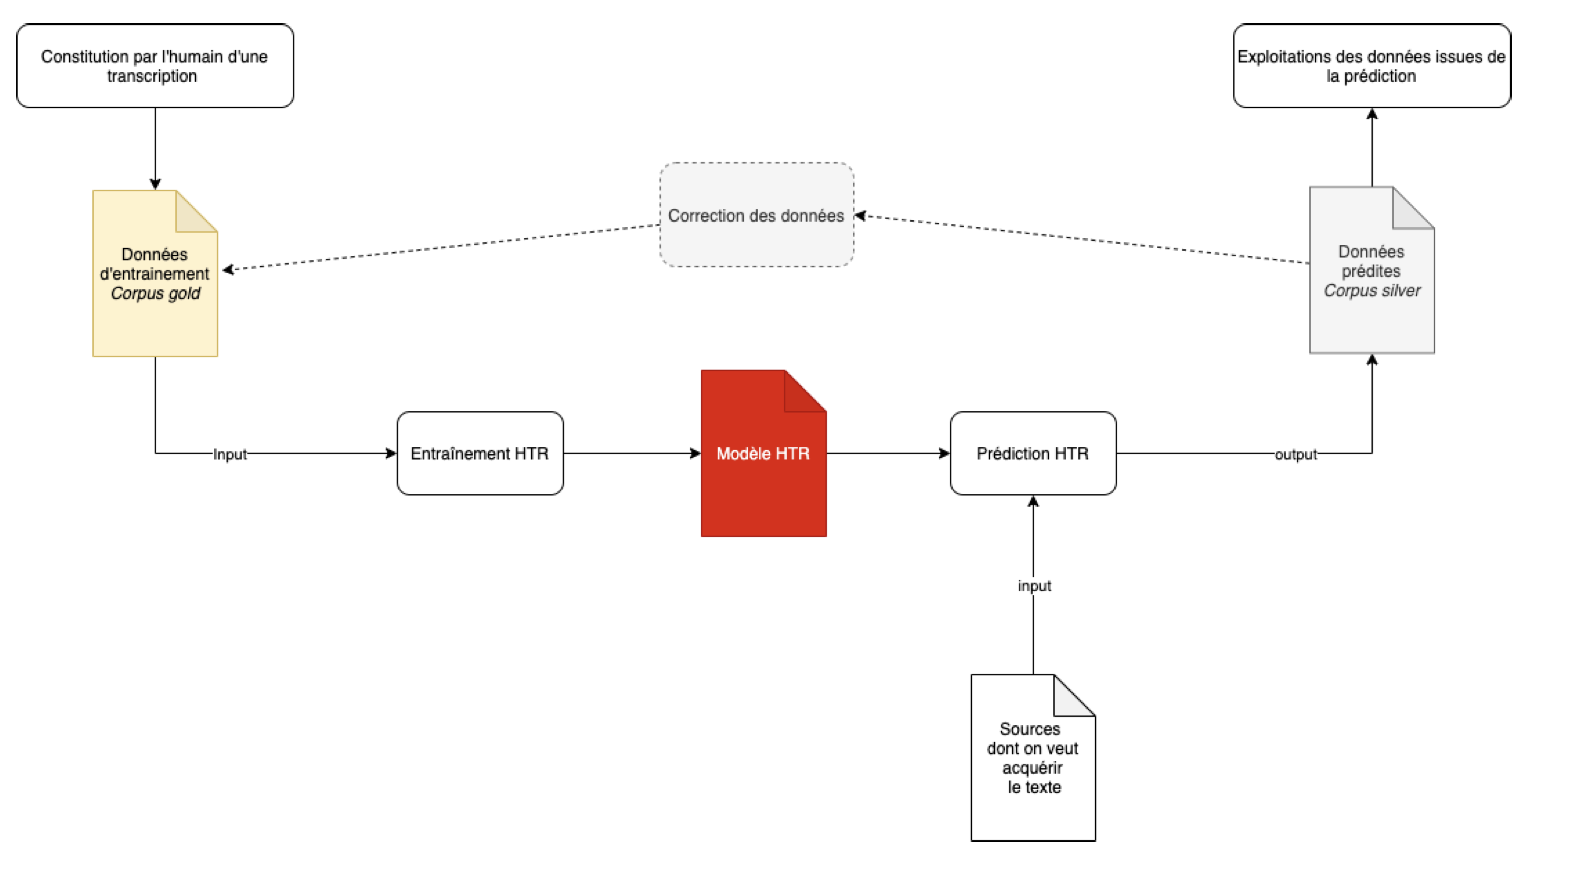
\includegraphics[width=0.7\linewidth]{images/schema_htr}
		\caption{Schéma d'un processus de reconnaissance d'écriture manuscrite.}
		\label{fig:schemhtr}
	\end{figure}
	
	Autre élément important dans le fonctionnement d’une chaîne de traitement HTR, c’est le moteur. Le moteur HTR est un système informatique conçu pour la reconnaissance et la transcription de texte manuscrit en format numérique. Ces moteurs utilisent des techniques avancées d’apprentissage automatique et de traitement d’image pour identifier et convertir les caractères manuscrits en texte exploitable. Le processus de reconnaissance de texte passe par plusieurs étapes. Tout d’abord, le retraitement des images pour améliorer la qualité du texte à reconnaître, incluant des ajustements tels que le redressement, la normalisation et la suppression du bruit. Ensuite, le texte est segmenté en lignes, mots et caractères individuels, ce qui est crucial pour isoler les éléments de texte dans l’image. La reconnaissance elle-même est effectuée à l’aide de modèles de deep learning qui analysent les segments de texte \footnote{Cf. Annexes, Figure \ref{fig:segmkrak}} pour identifier et transcrire les caractères. Après cette étape, des techniques de post-traitement sont appliquées pour corriger les erreurs et améliorer la précision du texte transcrit.
	\\
	
	Il est important de distinguer les termes « moteur » et « modèle ». Le moteur fait référence à l’ensemble du système complet, incluant les algorithmes, les outils ainsi que les processus nécessaires pour la reconnaissance de caractères manuscrits. Il englobe l’ensemble des pipelines de traitement, de l’entrée à la sortie, comme illustré par la chaîne de traitement dans le schéma. Cependant, il est possible que certains moteurs comme Kraken\footnote{ https://kraken.re/main/index.html} ou PyLaia\footnote{https://github.com/jpuigcerver/PyLaia/wiki}, deux moteurs HTR open-source, intègrent plusieurs modèles de reconnaissance et des techniques spécifiques pour traiter divers types de manuscrits et d’écritures. Tandis que le modèle se réfère spécifiquement aux architectures et aux algorithmes qui sont utilisés au sein du moteur pour effectuer la reconnaissance du texte. Ces derniers sont des composants clefs du moteur.

	Enfin, les “données prédites”, ou Corpus Silver, qui sont générées à la suite de la prédiction HTR, peuvent être exploitées pour diverses applications. Ces données, bien qu’elles puissent nécessiter des corrections, représentent une version numérique des textes manuscrits initialement inaccessibles et peuvent être intégrées dans d’autres systèmes pour une analyse plus approfondie ou pour enrichir des bases de données.
	\\
	
	Revenons à la chaîne de traitement. Une fois les documents analysés et jugés éligibles pour le traitement HTR, ils doivent être récupérés à l'aide d'un client FTP, comme précédemment décrit pour l'OCR. Une fois les documents récupérés, le traitement est réalisé à l'aide d'une application intégrant le moteur HTR Kraken. Ce programme permet d'abord de sélectionner les documents à traiter, puis de choisir le modèle HTR approprié. 
	\\
	
	\begin{figure}[h!]
		\centering
		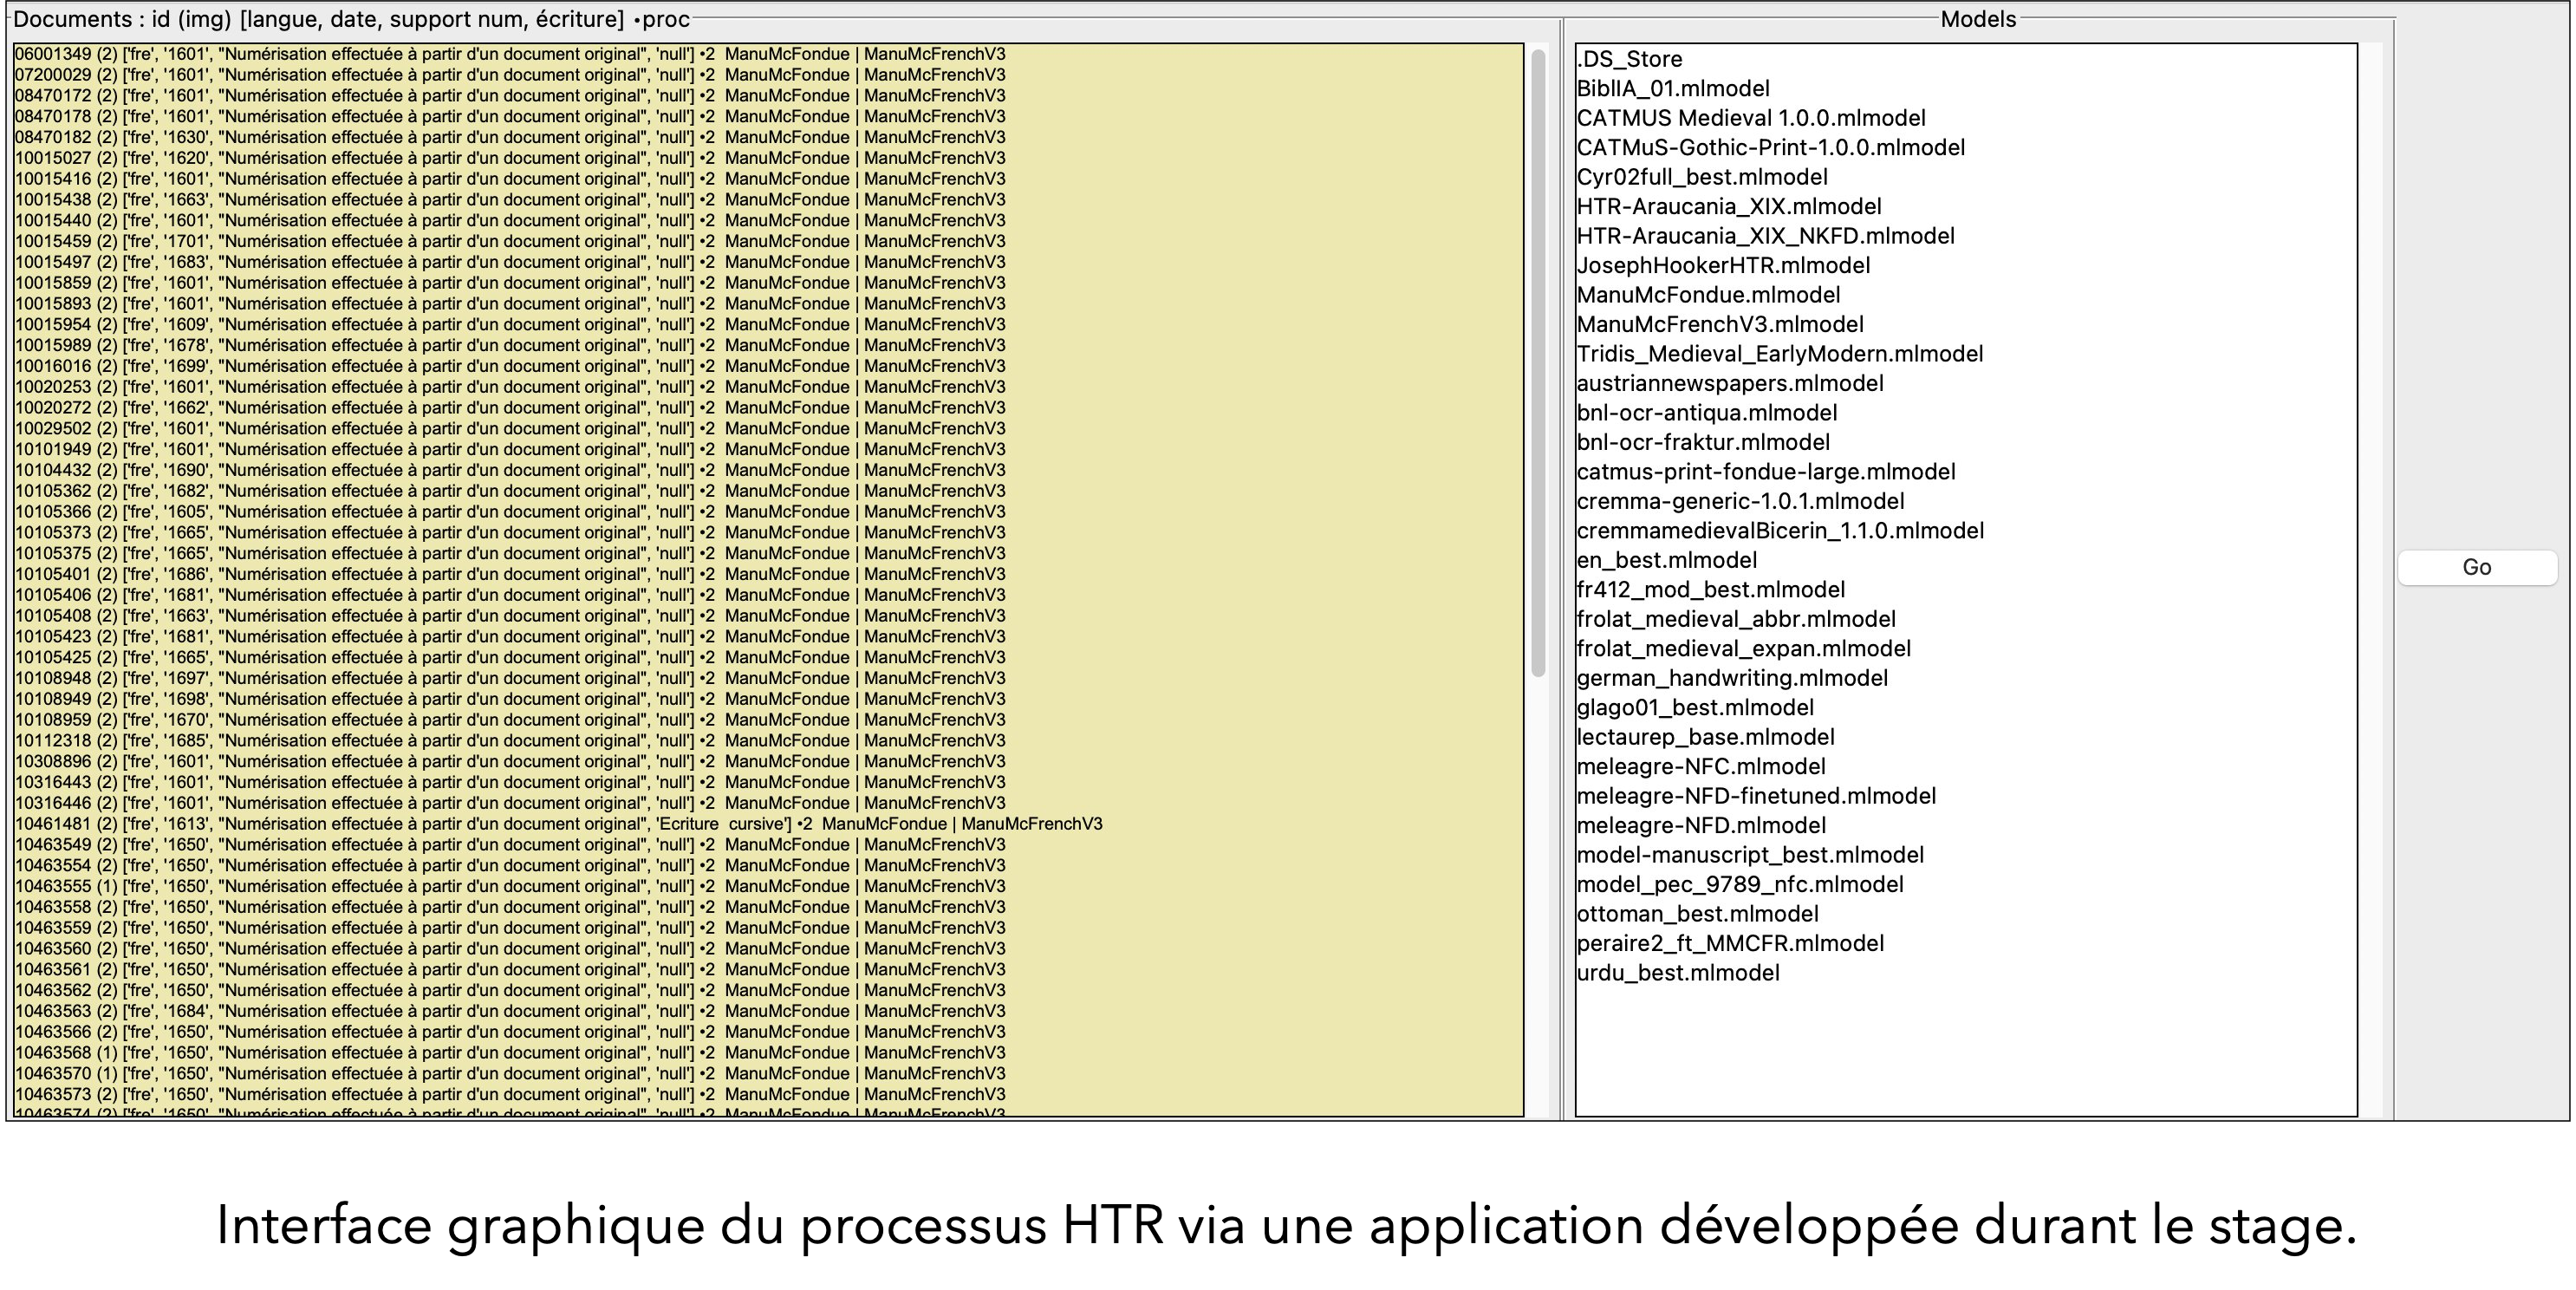
\includegraphics[width=0.8\textwidth]{images/app_htr_proc.png}
		\caption{Interface graphique du processus HTR via une application développée durant le stage.}
		\label{fig:monimage}
	\end{figure}
	
	Une fois le traitement terminé, l'application génère un dossier de sortie contenant un fichier XML au format ALTO. Ces fichiers ALTO \footnote{Cf. Annexes, Figure \ref{fig:altoxml}} sont précieux pour évaluer l'efficacité des modèles HTR sur une grande quantité de documents. Pour cela, les fichiers ALTO sont soumis à une application nommée « exploAlto » (eA), qui permet de réaliser une vérité de terrain (Ground Truth).
	
	Après avoir sélectionné et traité les documents jugés éligibles pour le traitement HTR, une étape cruciale consiste à évaluer la précision des transcriptions générées. Cette évaluation se fait grâce à l’utilisation de exploAlto, un programme spécialement conçu pour la création de la vérité de terrain, c’est-à-dire la validation et l’ajustement des transcriptions fournies par le moteur HTR.
	\\
	
	Le processus commence par le chargement des fichiers ALTO produits par le moteur HTR après le traitement des documents. Ces fichiers contiennent non seulement les transcriptions automatiques du texte manuscrit, mais aussi des informations cruciales sur la segmentation du document. La segmentation correspond à la manière dont le texte a été découpé en segments exploitables, tels que les lignes, les mots et les caractères individuels. C’est une étape déterminante, car la précision de cette segmentation influence directement la qualité de la transcription finale. Une fois les fichiers ALTO chargés, exploAlto affiche la segmentation réalisée par le moteur HTR. Cette étape permet à l’utilisateur de visualiser comment le modèle a interprété la structure du document manuscrit. Par exemple, les lignes de texte, les colonnes, ou les paragraphes sont identifiés et isolés, ce qui permet de s’assurer que le texte a été correctement segmenté avant d’être transcrit. Ensuite, exploAlto présente la retranscription du modèle HTR. Il s’agit du texte tel qu’il a été automatiquement reconnu par le modèle à partir de l’image du manuscrit. Cette retranscription est affichée en parallèle avec la segmentation du document, permettant ainsi de comparer directement le texte transcrit avec sa structure visuelle d’origine.
	\\
	
	À cette étape, l’utilisateur intervient pour corriger manuellement les erreurs détectées dans la retranscription. Cela peut inclure la rectification de caractères mal interprétés, de mots incorrects ou même de segments mal découpés. La correction manuelle est une étape essentielle, car elle permet de produire une transcription aussi fidèle que possible à l’original manuscrit. Ce processus de validation et de correction constitue ce que l’on appelle la vérité de terrain, une référence de haute qualité qui est utilisée pour évaluer la performance des modèles HTR. 
	Une fois les corrections effectuées, exploAlto calcule des métriques de performance pour évaluer la précision du modèle HTR. La métrique la plus importante dans ce contexte est le taux d’erreur par caractère (CER, pour Character Error Rate). Le CER est calculé en comparant le nombre de caractères mal transcrits au nombre total de caractères dans la vérité de terrain. Un CER faible indique que le modèle a bien réussi à transcrire les caractères, tandis qu’un CER élevé suggère un nombre significatif d’erreurs. La formule du CER est la suivante :
	
	\begin{center}
			$ CER = \frac{Nombre d'erreurs}{Nombre total de caractères} x 100 $
	\end{center}

	Enfin, exploAlto génère des rapports détaillés qui résument les performances du modèle HTR \footnote{Cf. Annexes, Figure \ref{fig:veritter}}. Ces rapports incluent des statistiques telles que le taux d’erreur par caractère et d’autres informations pertinentes sur la qualité de la transcription. Le CER, qui mesure le pourcentage d’erreurs de reconnaissance par rapport à la vérité de terrain, reste la métrique privilégiée pour évaluer la précision des transcriptions, en raison de sa sensibilité aux erreurs subtiles des caractères individuels.
	\\
	
	Cependant, le CER n’est pas la seule métrique utilisée pour évaluer la performance des modèles HTR. Une autre mesure couramment employée est le taux d’erreur au mot (WER, pour Word Error Rate). Le WER prend en compte les erreurs d’insertion, de suppression et de substitution de mots entiers, offrant ainsi une perspective différente sur la précision du modèle, bien qu’il soit généralement moins précis que le CER. En outre, il est également pertinent de considérer le Word Confidence (WC), qui évalue la confiance qu’a un modèle dans la reconnaissance correcte d’un mot spécifique dans un texte manuscrit. Le WC est une mesure clé pour évaluer et améliorer la performance des modèles HTR, car elle offre des informations précieuses sur la fiabilité des mots reconnus, aidant ainsi à gérer les erreurs potentielles dans le texte transcrit.
	
	Ces rapports produits par exploAlto sont essentiels pour comprendre les points faibles du modèle et identifier les domaines nécessitant des améliorations. Ils fournissent des données importantes pour optimiser les futurs traitements HTR, notamment dans le cadre de projets de transcription de masse, où la précision et l’efficacité sur un grand nombre de documents sont importantes.
	\\
	
	Les deux chaînes de traitement de la BnF, bien que visant toutes deux à extraire du texte à partir d'images, présentent des différences significatives dans leur mise en œuvre et leur portée. La chaîne OCR, solidement établie et intégrée aux systèmes de la BnF, traite les documents imprimés à grande échelle. Elle bénéficie d'une infrastructure robuste, avec des processus automatisés pour la sélection des documents, la gestion des flux et l'intégration des résultats dans les systèmes de la BnF comme SPAR et Gallica.
	
	En revanche, la chaîne HTR, conçue pour les manuscrits, fonctionne à une échelle plus réduite et de manière moins intégrée. Elle nécessite une approche plus ciblée pour la sélection des documents, s'appuyant sur une analyse approfondie des métadonnées. Le traitement HTR implique l'utilisation de modèles spécifiques adaptés aux différents types de manuscrits, contrairement à l'approche plus standardisée de l'OCR.
	
	La gestion des flux et l'évaluation des résultats diffèrent également entre les deux chaînes. Tandis que la chaîne OCR s'appuie sur des processus largement automatisés, la chaîne HTR implique davantage d'interventions manuelles et une évaluation plus poussée de la qualité des résultats, notamment à travers l'utilisation d'outils spécifiques pour la vérité de terrain.
	\\
	
	Ces différences reflètent non seulement la nature distincte des documents traités, mais aussi le niveau de maturité des technologies employées. L'OCR, technologie plus ancienne et éprouvée, bénéficie d'une intégration plus complète, tandis que le HTR, plus récent et complexe, reste en phase de développement et d'expérimentation au sein de la BnF et des établissements patrimoniaux en général.
	\\
	
	\subsection{OCR et HTR, seules face à la masse patrimoniale ? }
	
	L'utilisation de l'intelligence artificielle dans le domaine patrimonial ne se limite pas à l'OCR ou à l'HTR. L'avènement des LLMs (Large Language Models ou Grands Modèles de Langue) ouvre de nouvelles perspectives aux chercheurs et aux institutions. Ces modèles, intégrés au processus final de reconnaissance manuscrite, peuvent significativement améliorer l'efficacité des modèles HTR. En effet, l’une des applications prometteuses des LLMs est la correction des erreurs d’OCR, notamment pour les textes historiques, où les méthodes traditionnelles montrent souvent leurs limites.
	
	Par exemple, une étude menée par une équipe de l’Université de Stanford\footcite{manrique-gomez_historical_2024} met en avant l’utilisation de GPT-3.5 pour la correction d’OCR dans des journaux latino-américains du XIXe siècle. Ce modèle a permis d’améliorer la qualité des textes transcrits en corrigeant des erreurs que les systèmes OCR traditionnels n’auraient pas pu détecter, comme des erreurs de reconnaissance dues à l’usure des documents ou à des variations orthographiques propres à l’époque. Grâce à la capacité des LLMs à comprendre le contexte linguistique et historique, il devient possible de distinguer les véritables erreurs d’OCR des variations linguistiques authentiques, un défi majeur pour la transcription de documents anciens.
	En HTR, le développement de modèles généraux, non spécifiques à un style d’écriture ou à une période précise, permet d’avoir un volume de données de formation plus important. Cela offre une quantité textuelle plus grande, enrichissant ainsi la base de données pour entraîner les modèles. Les données créées par ces modèles peuvent ensuite être utilisées pour entraîner des LLMs dans des langues ou des domaines précis. De plus, l'aide des LLMs pour améliorer les modèles permet de développer des algorithmes généraux bien plus efficaces et précis, et ce, sur des périodes historiques plus larges.
	
	En avril 2023, Transkribus, une plateforme de reconnaissance de texte et de transcription automatique pour les documents historiques, développée par l'Université d'Innsbruck et actuellement gérée par READ-COOP\footcite{kahle_transkribus_2017}, a franchi une étape importante dans ce domaine. La plateforme a développé et publié deux modèles de LLMs : Dutchess I et GermanGiant I, tous deux issus d'un recyclage de modèles HTR généraux\footcite{nockels_implications_2024}. Dutchess I combine quatre modèles néerlandais couvrant une période allant du XVIIe au XIXe siècle. Entraîné par les Archives Nationales des Pays-Bas et celles d'Amsterdam, ce modèle atteint un impressionnant taux d'erreur de caractère de 4,3\%\footnote{ https://readcoop.eu/model/the-dutchess-i/ }. GermanGiant I, quant à lui, est formé à partir de modèles couvrant une période du XVIe au XXIe siècle en écritures latines et allemand kurrent, affichant un CER de 8,3\%\footnote{ https://readcoop.eu/model/the-german-giant-i/}. De plus, l’idée d’intégrer des grands modèles de langue déjà existants au lieu d'en développer de nouveaux a été analysée par Transkribus. En mai 2023, la plateforme a étudié comment intégrer ChatGPT\footcite{nockels_implications_2024} pour un traitement sur les sorties HTR, suite à des essais menés par la Bibliothèque municipale de Vienne sur des corrections de sorties HTR via les LLMs.
	
	L’intégration de ces outils et des jeux de données HTR, mêlés aux grands modèles de langue, ouvre la voie à de nouvelles méthodes de synthèse, de comparaison et d’analyse des données manuscrites. Néanmoins, l’adoption de bonnes pratiques pour profiter pleinement de ces avancées tout en évitant la perte du rôle intermédiaire de l’être humain dans le processus est cruciale. Il est important de développer des compétences en littératie informationnelle afin de distinguer correctement les informations émises par les machines des documents manuscrits humains, pour préserver la légitimité des sources principales. De plus, il est essentiel de développer des documentations détaillées pour assurer la transparence et la fiabilité des données et des processus.
	\\
	
	Cependant, bien que les LLMs offrent des perspectives prometteuses, leur utilisation dans la correction de textes OCR ou HTR présente certaines limites. Ces modèles, malgré leur puissance, peuvent souffrir de biais introduits par les corpus de formation modernes, ce qui peut conduire à des erreurs d’interprétation, particulièrement dans les textes historiques où les contextes linguistiques varient grandement. De plus, ils peuvent être sujets à des erreurs de surcorrection, modifiant des éléments textuels qui étaient en réalité corrects, ce qui peut altérer la fidélité des documents transcrits.
	
	En outre, l’utilisation des LLMs comporte des défis pratiques importants pour les établissements patrimoniaux, notamment en ce qui concerne les ressources matérielles et les coûts. Les LLMs nécessitent une puissance de calcul considérable, ce qui peut imposer des contraintes physiques, telles que le besoin de serveurs hautement performants et de solutions de stockage adaptées pour gérer les énormes volumes de données traitées. Ces infrastructures ne sont pas toujours accessibles aux institutions patrimoniales, en particulier celles disposant de ressources limitées. De plus, le coût financier de l’intégration des LLMs dans les processus de correction et de transcription peut être prohibitif. Les frais liés à l’acquisition des licences logicielles et à l’entretien des infrastructures technologiques sont élevés. Ces dépenses doivent être soigneusement pesées contre les avantages potentiels, en particulier dans un contexte où les budgets sont souvent restreints et les priorités multiples.
	
	Ces limitations soulignent l’importance d’une supervision humaine rigoureuse pour garantir que les corrections apportées par les LLMs préservent l’intégrité et l’authenticité des documents historiques. Ainsi, même avec les avancées offertes par les LLMs, leur utilisation doit être accompagnée de précautions et d’une validation humaine minutieuse pour maximiser la précision et la fiabilité des résultats. Il est également essentiel de prendre en compte les contraintes économiques et techniques associées à ces technologies pour assurer une adoption durable et bénéfique dans le domaine patrimonial.
	\\
	
	\part{Quatrième et dernière partie}}
	\chapter{Modèles génériques : quelle approche pour les corpus de la BnF ? }
	
	\lettrine{A}fin de traiter efficacement une grande quantité de documents manuscrits, les modèles HTR génériques apparaissent comme une solution logique pour les établissements patrimoniaux. Conçus pour surmonter les contraintes habituellement associées aux modèles spécifiques, ilsoffrent une flexibilité appréciable, capable de s’adapter à une diversité de périodes historiques, d’écritures et de langues. Cependant, cette flexibilité a aussi ses limites. L’efficacité de ces modèles, bien qu’optimale dans de nombreux cas, peut varier en fonction des caractéristiques spécifiques des documents traités. À travers une analyse des performances rencontrées lors de leur application sur un corpus varié de documents au cours du stage à la BnF, il est possible de mesurer la précision réelle de ces outils dans un contexte de traitement de masse. Les résultats obtenus montrent à la fois les points forts de ces modèles, mais aussi les défis qu’ils posent en termes de précision et d’adaptabilité. Par ailleurs, l’exploration des possibilités offertes par le fine-tuning, qui consiste à ajuster un modèle générique pour répondre aux spécificités d’un ensemble de données particulier, révèle une voie prometteuse pour les établissements souhaitant maximiser l’efficacité de leurs processus de transcription tout en répondant aux besoins uniques de leurs collections.
	
	\subsection{État de l'art des modèles génériques, ou des systèmes babéliens modernes.}
	
	Comme mentionné plus tôt, le stage réalisé au sein du département numérique de la BnF avait pour objectif de répondre à une question à première vue simple, mais dans le fond complexe : « Est-ce que les modèles génériques mis à disposition aujourd’hui par les chercheurs sont efficaces pour un traitement de masse ? ». 
	
	À première vue, si l’on s’intéresse aux retours des chercheurs sur le développement des modèles génériques, les résultats obtenus sur les jeux de données utilisés pour l’entraînement et l’affinement de ces modèles semblent plus que satisfaisants. C’est dans ce cadre que le projet CREMMA mérite une attention particulière. Ce projet se distingue par sa capacité à fournir une infrastructure et des outils collaboratifs qui repoussent les limites de la reconnaissance automatique des textes manuscrits. En mettant l’accent sur la mutualisation des ressources et le partage des connaissances, CREMMA favorise l’émergence de modèles plus robustes et universels, capables de s’adapter à une variété de matériaux anciens et de conditions d’application.
	
	CREMMA, pour Consortium pour la Reconnaissance d’Écritures Manuscrites des Matériaux Anciens, est un projet collaboratif financé par le DIM MAP\footnote{Domaine de recherche et d’innovation majeur (DIM) Matériaux anciens et patrimoniaux (MAP), un réseau de recherche francilien dédié l’étude des sciences du patrimoine, financé par la région Île de France. https://www.pamir.fr/}, visant à développer une infrastructure mutualisée pour la reconnaissance d’écritures manuscrites et la patrimonialisation numérique des textes anciens. En partenariat avec des institutions comme l’École nationale des chartes et l’Inria, CREMMA a déployé eScriptorium avec un budget dédié à l’acquisition de matériel performant. Le projet se distingue par son approche open source et sa volonté de partager les vérités de terrain et les modèles de transcription au sein de la communauté scientifique, contribuant ainsi à la démocratisation et à l’amélioration des pratiques en HTR\footcite{chague_cremma_2021}.
	
	
	Par exemple, pour le modèle Manu McFrench, développé dans le cadre du projet CREMMA, les chercheurs ont démontré que bien que ces modèles puissent effectivement offrir des taux de précision élevés, ces résultats dépendent fortement du type de documents traités et du contexte dans lequel ils sont utilisés. Ce modèle a été spécifiquement conçu pour la transcription de manuscrits français, couvrant une large période allant du XVIIe au XXIe siècle, avec une attention particulière portée aux écritures modernes et contemporaines. Le développement du modèle s’est appuyé sur une vaste collection de jeux de données diversifiés, incluant des manuscrits issus de différentes périodes historiques et contextes d’écriture, tels que les CREMMA Medii Aevi\footnote{Manuscrits en latin et vieux français de la période médiévale}, CREMMA Manuscrits du 17e, 18e, 19e et 20e siècles, ainsi que des données modernes comme CREMMA-Wikipedia\footnote{Corpus d'articles de la version française de Wikipédia} et les Testaments de Poilus\footcite{chague_manu_2023} . L’infrastructure mise en place par CREMMA, comprenant des serveurs performants et des outils tels que Kraken et eScriptorium, a permis d’entraîner le modèle rapidement et efficacement. Grâce à cette base solide, Manu McFrench a atteint un taux de reconnaissance des caractères de 90,56 \%\footcite{chague_manu_2023} sur leur ensemble de développement, illustrant son efficacité pour la transcription de textes manuscrits en français sur plusieurs siècles. Les études de cas, comme celles menées sur les journaux manuscrits de Lucien Peraire et les formulaires de recensement du Valais, ont révélé que les modèles génériques comme Manu McFrench permettent d’obtenir des scores d’exactitude améliorés, notamment en termes de taux d’erreur de caractère, tout en réduisant significativement le temps d’entraînement et les coûts associés à la transcription manuelle. De plus, la diversité des jeux de données utilisés a permis au modèle d’être particulièrement robuste face à une variété de styles d’écriture, rendant Manu McFrench un outil précieux pour les chercheurs et les institutions travaillant sur des collections manuscrites variées.
	
	Dans une perspective similaire à celle de Manu McFrench, le projet CATMuS (Consistent Approaches to Transcribing Manuscripts) Medieval, se concentre sur la création d’un modèle de reconnaissance d’écritures manuscrites multilingues, couvrant une vaste période allant du VIIIe au XVIe siècle. Le corpus d’entraînement de CATMuS, qui comprend 200 manuscrits et incunables représentant 160 000 lignes de texte et 5 millions de caractères, constitue une base rigoureuse pour l’optimisation des modèles HTR. Les résultats obtenus par les modèles Kraken et PyLaia sur ce dataset sont révélateurs : Kraken a atteint un CER de 4,51 \%, tandis que PyLaia a légèrement surpassé ce résultat avec un CER de 3,89 \%. Ces chiffres démontrent l’efficacité de ces modèles pour traiter des manuscrits historiques complexes, tout en soulignant l’importance de la constitution du corpus d’entraînement pour garantir des performances optimales. 
	
	Un autre aspect crucial à considérer dans l’évaluation des modèles HTR génériques est leur performance en termes de précision et leur capacité à s’adapter à différents types de documents historiques. Le projet CREMMALab, dans ce contexte, se distingue par le développement de plusieurs modèles de transcription, dont Bicerin et Cortado, qui visent à fournir des outils robustes pour la reconnaissance de manuscrits médiévaux\footcite{pinche_generic_2023}.
	
	Le modèle Bicerin, développé sous la supervision d’Ariane Pinche, est spécifiquement conçu pour la reconnaissance de textes dans des manuscrits médiévaux. Ce modèle s’appuie sur un ensemble de données soigneusement sélectionnées, principalement issues de sources médiévales, afin d’optimiser la reconnaissance des écritures de cette période. Avec une précision de 95,49 \%\footcite{pinche_images_2022} en termes de taux d’erreur de caractère, Bicerin démontre une capacité impressionnante à gérer la complexité et la variabilité des écritures médiévales. Ce modèle illustre ainsi la réussite des approches génériques lorsqu’elles sont appliquées à des corpus bien définis et homogènes, tout en soulignant l’importance de la qualité du corpus d’entraînement pour atteindre de tels résultats.
	
	De son côté, le modèle Cortado 2.0.0 pousse l’idée de l’intégration et de la mixité des datasets encore plus loin. Ce modèle combine le dataset CREMMA Medieval avec des impressions anciennes du XVe siècle issues du projet Gallic(orpor)a, un projet qui vise à transcrire et rendre accessibles les textes imprimés anciens. L’objectif de cette approche est de créer un modèle générique capable de traiter non seulement les manuscrits médiévaux, mais aussi les premières impressions typographiques, étendant ainsi l’utilité du modèle à une plus grande variété de documents historiques. Avec une précision légèrement supérieure à celle de Bicerin, atteignant 95,54 \% de précision\footcite{pinche_htr_2022}, Cortado 2.0.0 montre que l’intégration de datasets variés peut effectivement améliorer la performance d’un modèle générique, tout en le rendant plus flexible pour différentes typologies de documents. Cependant, ce résultat souligne également la nécessité d’une approche rigoureuse dans la sélection des datasets pour s’assurer que le modèle reste performant sur un large éventail de documents.
	\\
	
	Bien que les résultats soient prometteurs, ils mettent en lumière les défis restants, notamment liés à la diversité des écritures et à la qualité des documents numérisés. Ainsi, CATMuS, à l’instar de Manu McFrench, illustre que les modèles génériques peuvent offrir des bases solides pour la transcription de textes anciens, mais leur efficacité ultime repose sur une adaptation fine aux spécificités des documents traités.
	\\
	
	Si nous avons abordé des projets de la communauté scientifique française, ou du moins francophone, d’autres projets internationaux font ressortir aussi les mêmes problématiques. 
	
	Penchons nous sur la question allemande et les modèles génériques pour la reconnaissance du Kurrent allemand du XIXe siècle\footcite{hodel_general_2021}. Tobias Hodel et ses collègues ont démontré que la performance des modèles génériques est intrinsèquement liée à la qualité et à la diversité des corpus d’entraînement. Les taux d’erreur de caractère observés varient entre 1,73 \% et 6,53 \%, selon les ensembles de test et les moteurs utilisés. Ces résultats soulignent non seulement l’efficacité potentielle des modèles génériques, mais aussi les limites de leur généralisation à des écritures non vues auparavant. Ainsi, tout comme pour les projets français, l’efficacité des modèles HTR dépend fortement de l’adéquation entre le corpus d’entraînement et les spécificités des documents à traiter. 
	
	Du côté finnois, les archives nationales de Finlande (NAF) ont mené un projet de recherche afin de développer un modèle de reconnaissance de texte manuscrit basé sur le Transformer, comme pour le projet READ\_CHINESE vu plus haut. Ici, c’est le modèle TrOCR qui est utilisé afin de transcrire des documents historiques en finnois et en suédois couvrant une période allant du XVIIe au XXe siècle. Le Transformer se distingue des approches traditionnelles en ce qu’il utilise un mécanisme d’attention qui permet de diviser l’image en plusieurs petites parties, appelées patches, et de traiter chacune de ces parties pour en extraire les informations nécessaires à la reconnaissance du texte\footcite{li_trocr_2023}. Ensuite, le texte est généré à partir de ces informations en s’appuyant sur des modèles de langage déjà entraînés.
	\\
	\begin{figure}[h!]
		\centering
		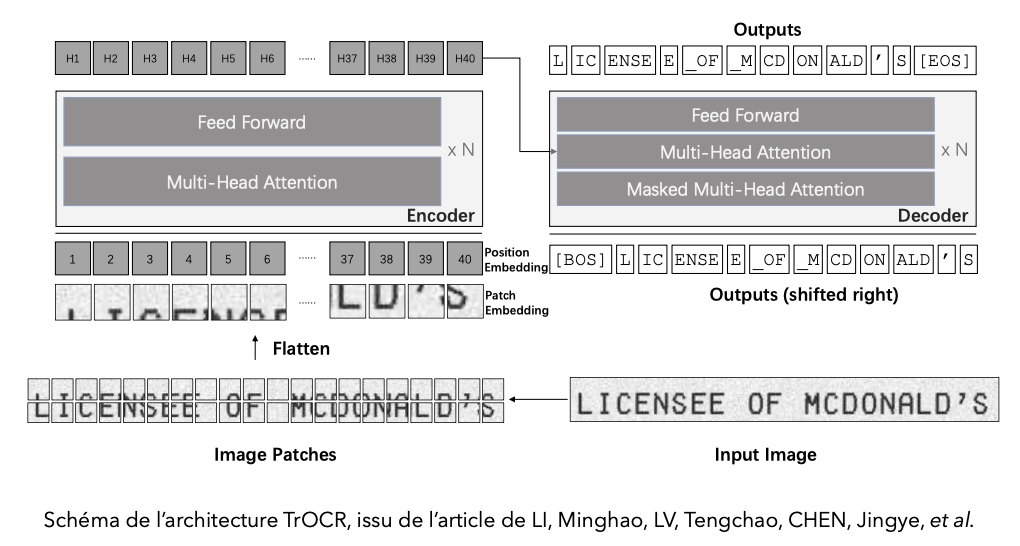
\includegraphics[width=0.8\textwidth]{images/TrOcr_schem.png}
		\caption{Schéma de l’architecture TrOCR, issu de l’article de LI, Minghao, LV, Tengchao, CHEN, Jingye, et al. }
		\label{fig:monimage}
	\end{figure}
	
	Le schéma de l’architecture TrOCR illustre ce processus : chaque image est d’abord segmentée en patches, qui sont ensuite transformés en séquences de données traitées par l’encodeur du Transformer. L’encodeur applique une attention multi-tête pour identifier les relations entre les différentes parties de l’image, puis utilise des couches feed-forward pour affiner et enrichir la représentation des données. Ces couches feed-forward jouent un rôle clé en appliquant des transformations linéaires suivies de fonctions d’activation, permettant ainsi de capturer les caractéristiques essentielles du texte à reconnaître. Enfin, le décodeur génère la transcription du texte en se basant sur cette représentation raffinée\footcite{riikka_handwritten_nodate}.
	
	Contrairement aux méthodes plus classiques, qui reposent sur des réseaux de neurones convolutifs (CNN) pour analyser l’image et des réseaux de neurones récurrents (RNN) pour produire le texte, le Transformer intègre ces deux étapes en une seule. Cette intégration simplifie le processus tout en offrant des performances améliorées, ce qui en fait une technologie particulièrement adaptée pour la transcription de documents historiques complexes, comme ceux traités par les archives nationales de Finlande. Néanmoins, cette performance n’est pas sans enjeux, car elle requiert une puissance de calcul considérable, notamment en termes de ressources GPU (Graphic Processing Units ou Unité de traitement graphique). Les modèles basés sur l’architecture Transformer, en intégrant le traitement des images et la génération de texte en une seule étape, sollicitent intensivement les capacités de calcul pour gérer les opérations complexes de self-attention et de traitement parallèle des données. Cette exigence en puissance de calcul est particulièrement prononcée lors de l’entraînement du modèle, où de grandes quantités de données doivent être traitées de manière simultanée\footcite{li_trocr_2023}.
	\\
	
	Autre projet européen, aux Pays-Bas, on se pose la question, au travers du projet ARIetta, de la conception d’un « supermodel » permettant la reconnaissance de textes manuscrits en néerlandais historique\footcite{lefranc_arletta_2024}. S’il n’est pas à proprement parler un modèle générique, il permet tout de même de traiter une masse de documents importante sur une période large allant du XVIIe au XXe siècles provenant de différents projets néerlandophone. Cette approche d’entraînement sur un ensemble diversifié de données historiques a pour but de rendre le modèle plus polyvalent et capable de traiter une variété de documents manuscrits, même s’ils proviennent de différentes époques ou qu’ils présentent des styles d’écriture variés. Ce « supermodel » est aussi présenté comme une base pour d’autres projets de transcription, faisant de lui un « foundational model », un modèle fondamental, permettant de créer de nouveaux modèles à partir ce celui-ci, comme un point de départ afin de minimiser le temps et les efforts pour les chercheurs. 

	\\
	
	En somme, les modèles génériques offrent des avantages indéniables dans le domaine de la reconnaissance de texte manuscrit, notamment par leur capacité à s’adapter à une grande variété de documents et d’écritures. Comme le montrent les résultats obtenus avec les modèles Manu McFrench, CATMuS, Bicerin, et Cortado, ces modèles peuvent considérablement améliorer la précision des transcriptions tout en réduisant le temps et les coûts associés. Cependant, leur efficacité dépend fortement de la qualité et de la diversité des jeux de données utilisés pour leur entraînement, ainsi que de leur adéquation avec les spécificités des documents à traiter.
	
	De plus, selon l’objectif de l’utilisateur, l’impact de la précision d’un modèle générique peut varier. Par exemple, une précision supérieure à 85 \% peut suffire pour des tâches de text mining, tandis que pour la production d’éditions ou l’accélération de la transcription, des scores supérieurs à 95 \% sont souvent nécessaires. Les modèles génériques ne sont toutefois pas toujours destinés à être utilisés directement. Ils peuvent également servir de base pour un fine-tuning efficace, permettant d’atteindre des taux de précision supérieurs à 98 \% avec seulement quelques pages d’entraînement supplémentaires. Ce processus permet de personnaliser rapidement un modèle générique pour l’adapter à un corpus spécifique, que ce soit dans une autre langue, un autre type d’écriture, ou même pour des images de qualité inférieure\footcite{pinche_generic_2023}.
	
	Malgré ces avantages, l’application de ces modèles à des corpus variés, tels que ceux de la BnF, pose la question de leur capacité à maintenir une haute précision dans des contextes moins contrôlés. C’est cette analyse que nous aborderons dans la sous-partie suivante, en examinant les performances de ces modèles génériques sur un corpus hétérogène de documents issus de la BnF.
	\\
	
	\subsection{Des modèles théoriques à la pratique : Analyse des performances des modèles génériques sur un corpus de manuscrits de la BnF}
	
	Comme nous l’avons observé, les modèles génériques développés par les chercheurs sont entraînés sur des corpus spécifiques, constitués de larges jeux de données conçus pour affiner les modèles en fonction des particularités des manuscrits. Au cours de mon stage, j’ai mis en place une chaîne de traitement HTR afin d’évaluer l’efficacité des modèles génériques actuellement disponibles pour le traitement d’un volume important de documents. Pour rappel, la BnF possède un vaste patrimoine de 203 252 manuscrits numérisés, couvrant une grande diversité de langues et une vaste période historique, allant d’avant notre ère jusqu’à la fin du XXe siècle. Cependant, dans le cadre du stage, l’analyse s’est concentrée sur un corpus plus restreint, limité à des manuscrits français datés du XVIIe au XIXe siècle, tous numérisés à partir d’originaux. Ce choix a réduit le corpus étudié à 9 867 documents.
	\\
	
	Afin de répondre à la problématique, un échantillon de ce corpus a été utilisé pour étudier l’efficacité de deux modèles : Manu McFrench V3 et Manu McFondue\footnote{ Gabay (S.), Chagué (A.) et Clérice (T.), HTR-United - Manu Mc Fondue (Manuscripts of Modern and Contemporaneous French - Manu McFrench v4) (Version v4), Zenodo, 2024. URL : https://doi.org/10.5281/zenodo.10886224.}. Manu McFondue est un modèle développé dans le cadre du projet FoNDUE (FOrmes Numérisées et Détection Unifiée des Écritures)\footnote{https://github.com/FoNDUE-HTR/Documentation} à l’Université de Genève. Financé par la Faculté des lettres et le COINF de l’université, il utilise eScriptorium, un logiciel open source soutenu par le moteur HTR Kraken, pour la reconnaissance d’écritures manuscrites.

	Ces deux modèles génériques, multilingues et couvrant différentes époques, se sont révélés des candidats pertinents pour le traitement du corpus réduit. L’analyse des performances des modèles HTR appliqués aux manuscrits numérisés de la BnF a permis de produire des données précieuses, montrant que Manu McFondue et Manu McFrench V3 ont obtenu des résultats globalement satisfaisants, mais avec des variations notables selon les documents. L’évaluation a été réalisée en se basant sur le taux d’erreur corrigé, une métrique clé qui mesure le pourcentage de caractères nécessitant une correction après la transcription automatique.
	
	Le tableau ci-dessous résume les résultats obtenus pour ces deux modèles en termes de documents traités, de nombre total de lignes, de lignes corrigées, ainsi que la précision moyenne, minimale et maximale :
	

\begin{table}[h]
	\centering
	\resizebox{\textwidth}{!}{%
		\begin{tabular}{|l|c|c|c|c|c|c|}
			\hline
			\textbf{Modèle} & \textbf{Doc. traités} & \textbf{Lignes totales} & \textbf{Lignes corrigées} & \textbf{CER Moyen} & \textbf{CER Max} & \textbf{CER Min} \\ \hline
			ManuMc Fondue.mlmodel & 69 & 3586 & 2684 & 0.1394 & 0.31 & 0.05 \\ \hline
			ManuMc FrenchV3.mlmodel & 21 & 1134 & 757 & 0.1376 & 0.27 & 0.04 \\ \hline
		\end{tabular}%
	}
	\caption{Performances des modèles ManuMc Fondue et ManuMc FrenchV3.}
	\label{table:performances}
\end{table}

	
	Ces résultats montrent que les deux modèles offrent des performances globalement similaires en termes de précision moyenne, ManuMcFrenchV3 ayant des performances légèrement meilleures en termes de CER minimum et maximum. \textit Cependant, en raison du manque de temps, de main-d’œuvre, et de la grande quantité de documents à traiter, il existe une différence significative dans le nombre de documents traités par chaque modèle. Chaque document doit être traité et validé deux fois, une fois par modèle. Face à cette contrainte, il a été décidé de se concentrer principalement sur ManuMcFondue, car il s’agit d’un modèle plus récent, et les résultats observés étaient relativement proches de ceux de ManuMcFrenchV3.
	\\
	
	Le modèle ManuMcFondue a affiché une large gamme de performances, avec un CER allant de 8 à 31\% selon les manuscrits. Par exemple, pour des documents comme le btv1b525094323\footnote{Perrault, Claude. « Sçavoir si la musique à plusieurs parties a esté connüe et mise en usage par les Anciens. » Manuscrit, XVIIe siècle, 42 pages, 215 × 160 mm. Reliure en veau gr. Manuscrit en français. Cote : Français 25350 (ancienne cote : Notre-Dame 280). Bibliothèque nationale de France, Département des Manuscrits. https://gallica.bnf.fr/ark:/12148/btv1b525094323,  cf Annexes, figure \ref{fig:mssbnfex1}}, un manuscrit du XVIIe siècle, le modèle a atteint un CER de 8\%, ce qui témoigne d’une très bonne précision, suggérant que les caractéristiques du texte étaient bien adaptées aux capacités du modèle. 	À l’inverse, pour des manuscrits plus difficiles comme le btv1b10015954z\footnote{Arrêt du Parlement permettant aux habitants de Vauvert de faire paître dans la Selve. Manuscrit, 28 juin 1609, 10 feuillets, 28 cm. Manuscrit en français. Cote : Ms\_354\_22. Bibliothèque nationale de France, Département des Manuscrits.	 https://gallica.bnf.fr/ark:/12148/btv1b10015954z, cf Annexes, figure \ref{fig:mssbnfex2}}, le CER a grimpé à 0,3, indiquant que près de 30 \% des caractères ont dû être corrigés, probablement en raison de la complexité du texte ou de la qualité médiocre de la segmentation.
	\\
	\begin{figure}[h!]
		\centering
		\begin{minipage}{0.45\textwidth}
			\centering
			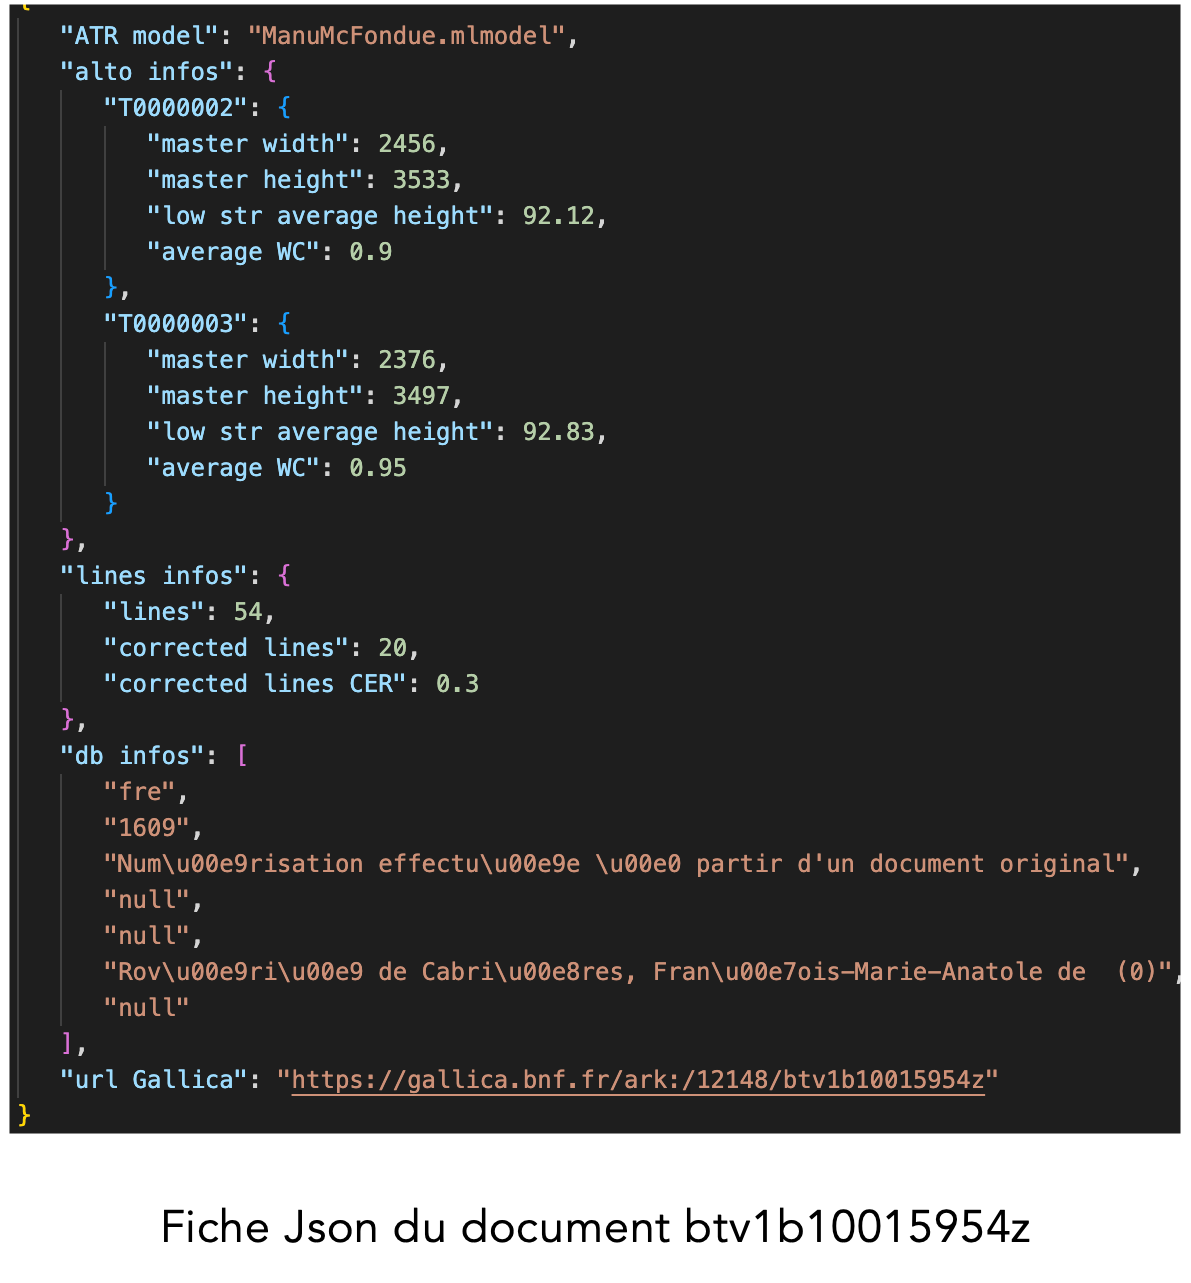
\includegraphics[width=\textwidth]{images/fiche_json_a.png}
			\caption{Fiche Json du document btv1b10015954z }
			\label{fig:image1}
		\end{minipage}\hfill
		\begin{minipage}{0.45\textwidth}
			\centering
			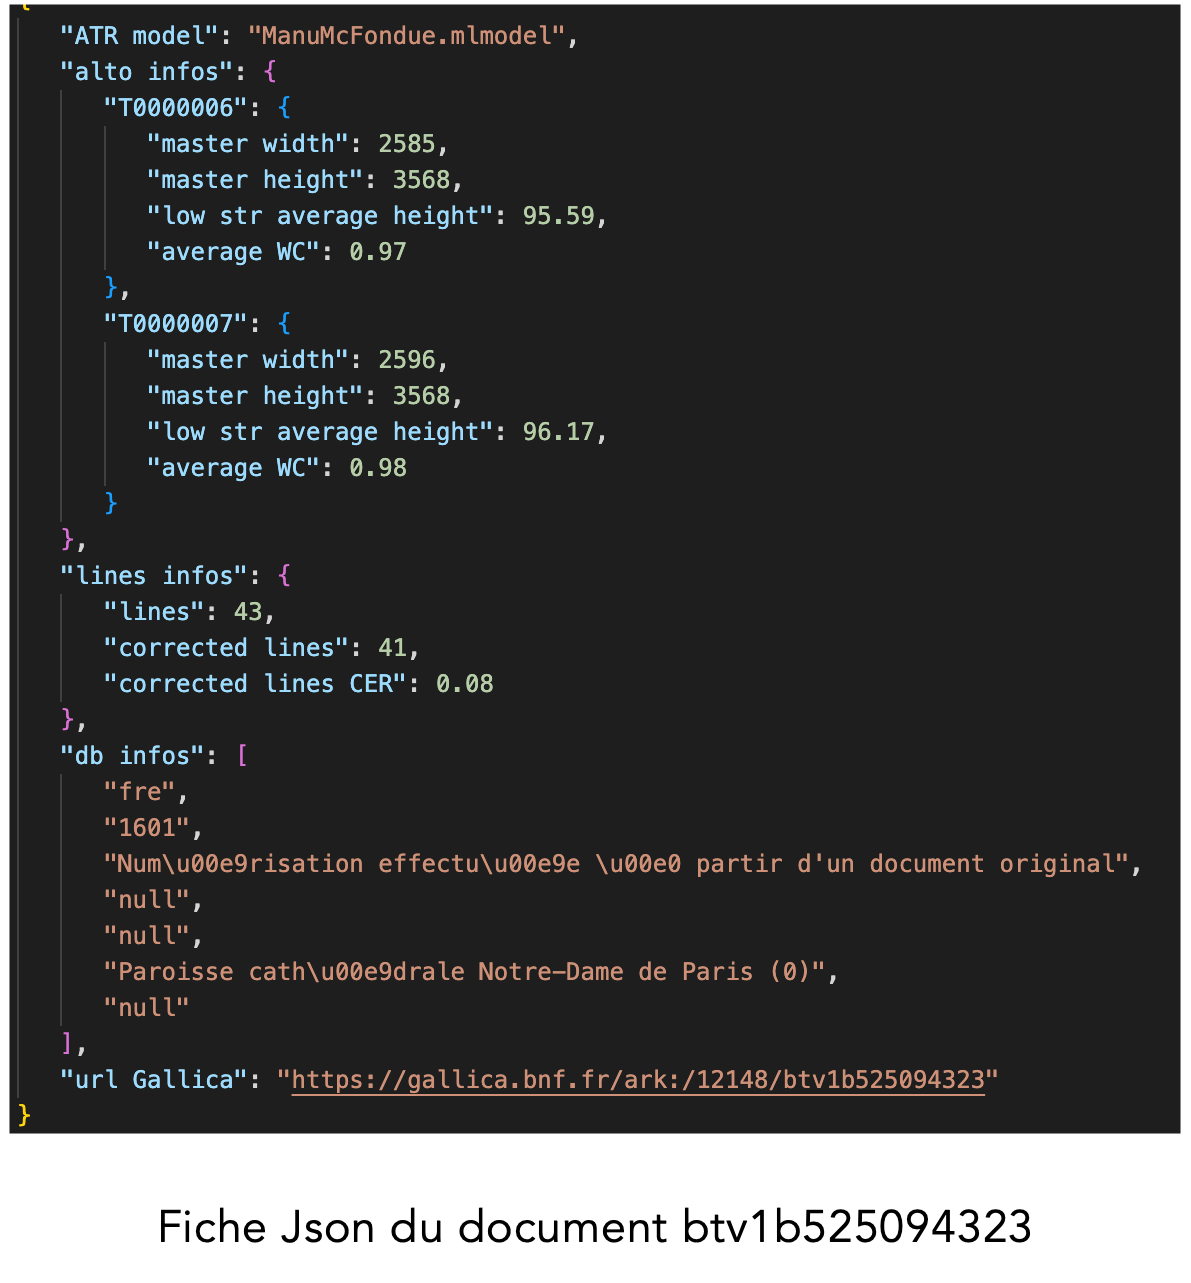
\includegraphics[width=\textwidth]{images/fiche_json_a1.png}
			\caption{Fiche Json du document btv1b525094323 }
			\label{fig:image2}
		\end{minipage}
		\caption{Fiches JSON des documents sous modèles McFondue}
		\label{fig:images_cote_a_cote}
	\end{figure}
	
	Le modèle ManuMcFrenchV3 a, quant à lui, montré des performances légèrement supérieures en moyenne, avec des CER allant de 4 à 31\%. Sur des manuscrits bien numérisés et relativement faciles à lire, comme le document btv1b84701789\footnote{De Valles, sieur. « Recueil des armoiries de tous les admiraux de France qui ont esté successivement creés, depuis leur institution en tiltre d’office, jusques au regne de tres hault, tres puissant et tres magnanime prince Louis, 13e du nom… par le sieur DE VALLES, de la ville de Chartres ». Manuscrit, XVIIe siècle, Papier, portrait, armoiries coloriées. Manuscrit en français. Cote : Français 2767 (ancienne cote : Anc. 8358). Bibliothèque nationale de France, Département des Manuscrits.  https://gallica.bnf.fr/ark:/12148/btv1b84701789, Cf. Annexes, Figure \ref{fig:mssbnfex3}}, le modèle a atteint un CER exceptionnel de 4\%, illustrant une reconnaissance quasi parfaite du texte. Cependant, sur des documents plus complexes ou de qualité inférieure, les résultats étaient comparables à ceux de ManuMcFondue, avec un CER pouvant également atteindre 31\%.
	\\
	\begin{figure}[h!]
		\centering
		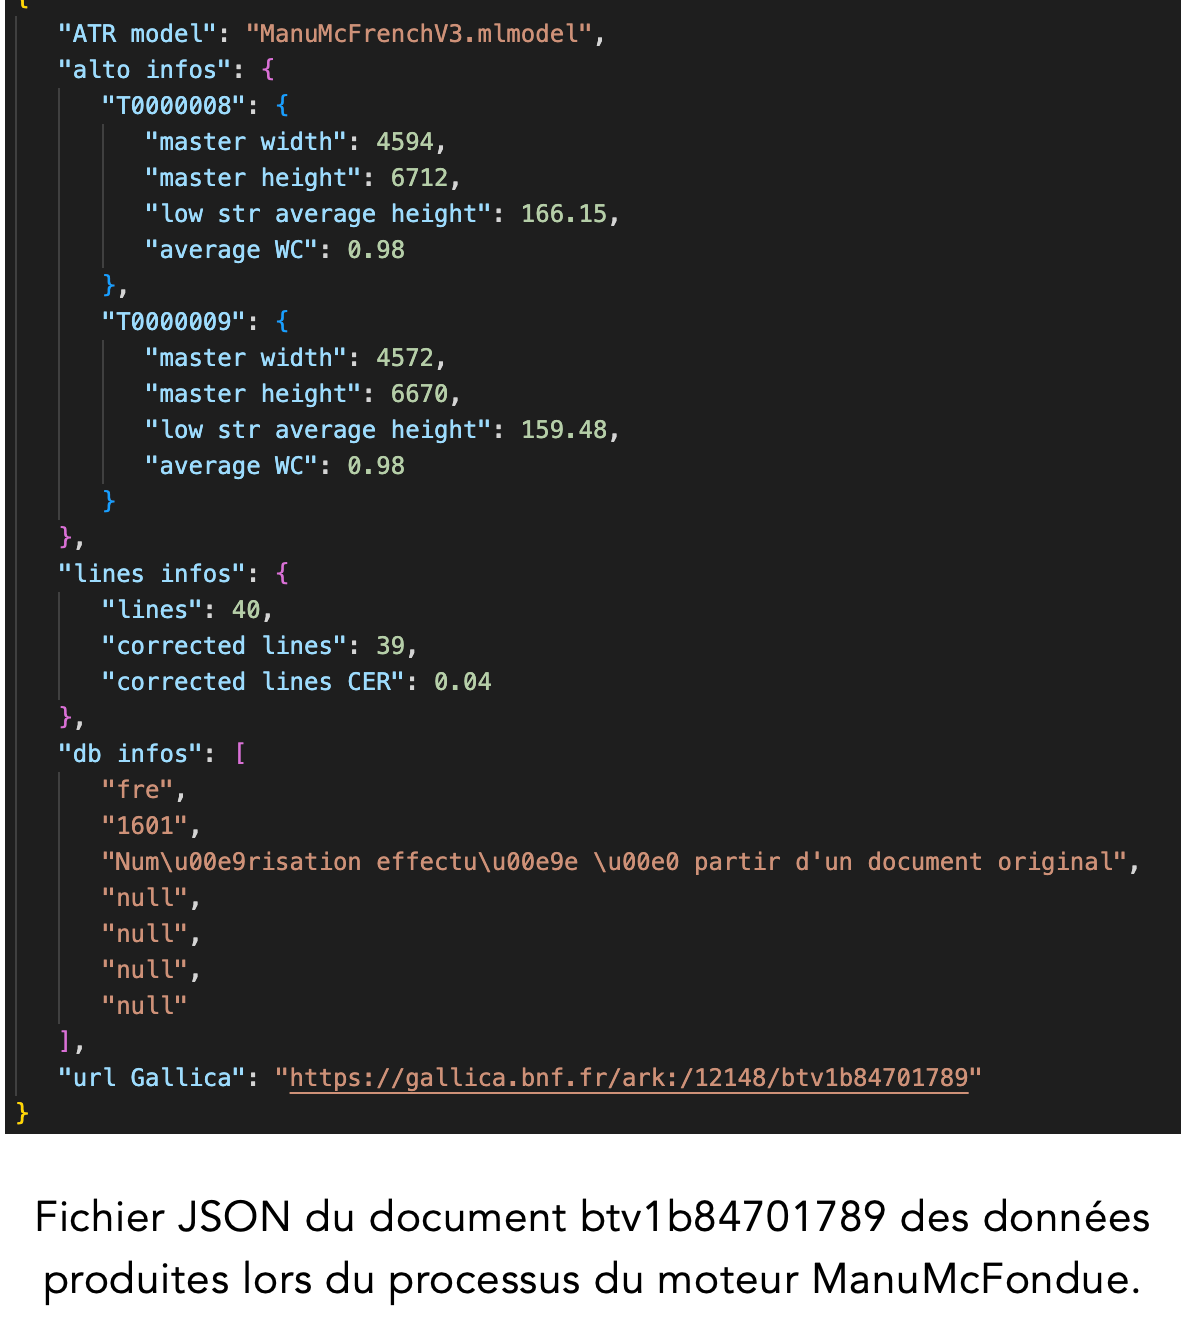
\includegraphics[width=0.8\textwidth]{images/fiche_json_b.png}
		\caption{Fichier JSON du document btv1b84701789 des données produites lors du processus du moteur ManuMcFrench V3.}
		\label{fig:monimage}
	\end{figure}
	
	En moyenne, ManuMcFondue a affiché un CER moyen d’environ 18\%, tandis que ManuMcFrenchV3 a légèrement mieux performé avec un CER moyen de 14\%. Ces moyennes montrent que, bien que les deux modèles soient compétitifs, ManuMcFrenchV3 semble offrir une meilleure précision globale sur l’ensemble du corpus testé.
	\\
	
	Ces résultats révèlent que bien que les modèles génériques puissent fournir une base solide pour la transcription de manuscrits, leur performance optimale reste fortement dépendante de la qualité et des caractéristiques spécifiques des documents traités. Les taux d’erreur plus élevés sur certains manuscrits soulignent l’importance de personnaliser et d’affiner les modèles pour maximiser leur efficacité. En particulier, le fine-tuning pourrait permettre d’améliorer significativement les résultats pour les documents les plus complexes, en adaptant les modèles aux particularités des corpus spécifiques de la BnF.
	\\
	
	Dans l’ensemble, cette analyse met en évidence la nécessité d’une approche nuancée lorsqu’il s’agit d’appliquer des modèles génériques à des collections variées comme celles de la BnF. Si ces modèles montrent des résultats prometteurs, leur utilisation dans un contexte de traitement de masse requiert une attention particulière aux spécificités des documents, ainsi qu’une potentielle adaptation pour garantir une reconnaissance textuelle fiable et précise. Et dans ce cas ci, il est possible dese demander si le fine-tuning des modèles sur les corpus spécifiques de la BnF ne serait pas une solution pour traiter certains ensembles documentaires, tels que les manuscrits en arabe ou en arménien, afin de rendre ces documents plus accessibles au plus grand nombre ? 
	
	\subsection{D'un modèle général à un modèle spécifique : le \textit{fine-tuning}.}
	
	Un point définition s’impose avant toute chose. Le fine-tuning peut être décrit comme étant un processus qui consiste à affiner et adapter les paramètres d’un modèle pré-entraîné sur une tâche similaire à celle ciblée par l’utilisateur. Cette méthode permet de limiter significativement le nombre de données nécessaires pour obtenir un modèle performant, par opposition à la création d’un modèle de zéro (from scratch). Le fine-tuning est particulièrement efficace lorsque l’on dispose déjà d’un modèle pré-entraîné sur une langue ou un type de document similaire, car il permet d’obtenir rapidement un modèle adapté à des conditions spécifiques avec un minimum de données supplémentaires\footcite{vidal-gorene_reconnaissance_2023} . 
	\\
	
	Les schémas\footcite{vidal-gorene_reconnaissance_2023} suivants illustrent parfaitement les différences entre l’entraînement d’un modèle OCR/HTR de zéro et la spécialisation d’un modèle pré-entraîné via le processus de fine-tuning. L’entraînement d’un modèle à partir de zéro est un processus complexe et coûteux en termes de temps et de ressources. Il débute par la constitution de la “vérité terrain”, où chaque image de document numérisé est associée à sa transcription manuelle. Ces données, une fois préparées, sont divisées en deux ensembles distincts : l’ensemble d’apprentissage et l’ensemble de test. Le modèle est ensuite formé de manière itérative sur l’ensemble d’apprentissage, avec pour objectif de minimiser les erreurs de prédiction. Une fois finalisé, il est évalué sur l’ensemble de test avant d’être appliqué à des documents similaires pour en extraire automatiquement le texte. Cette approche, bien qu’efficace, nécessite un volume de données conséquent et un processus d’entraînement long.
	\\
	\begin{figure}[h!]
		\centering
		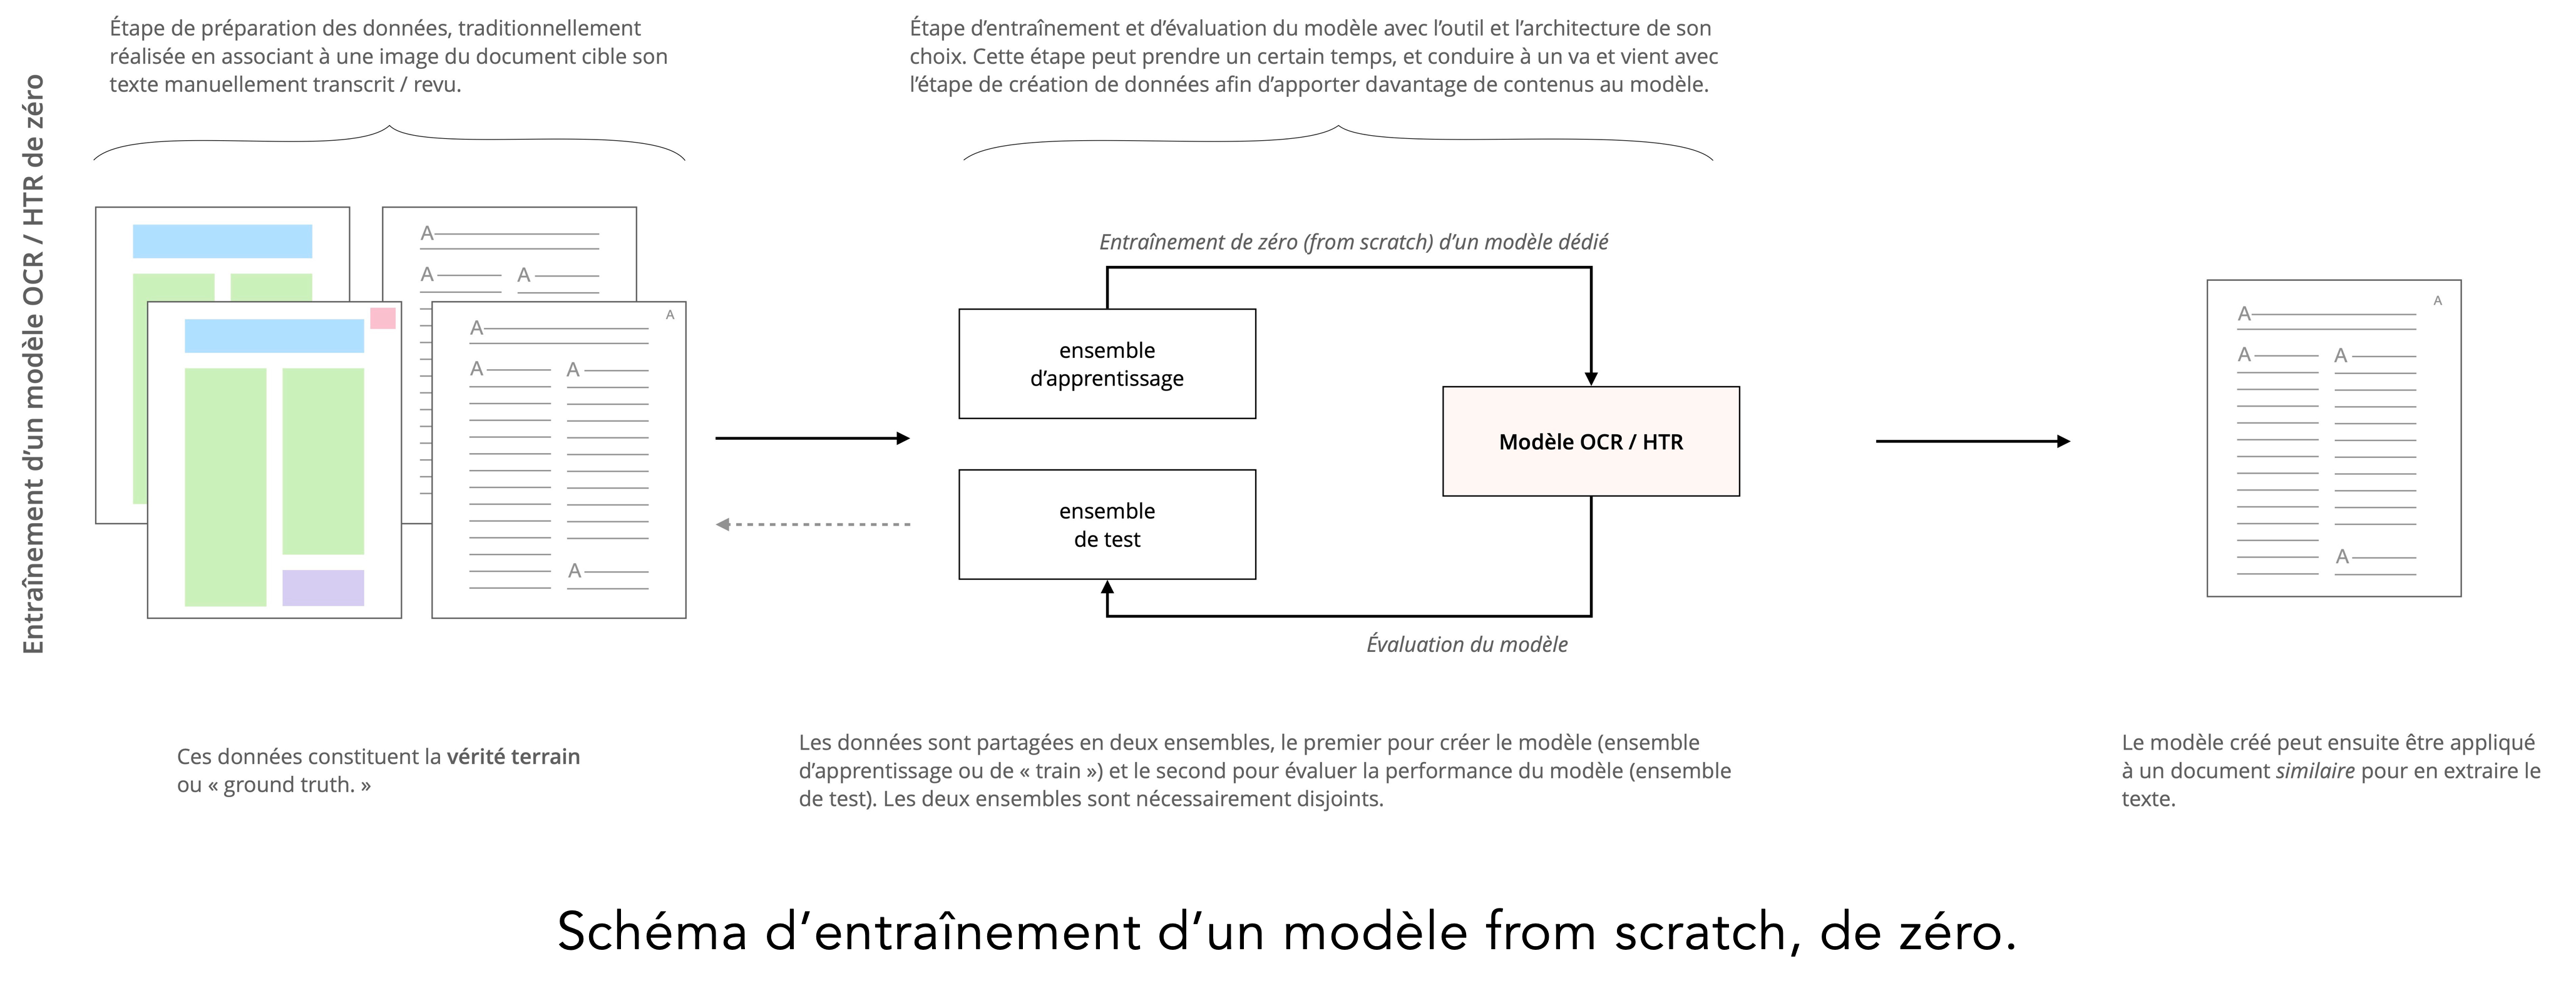
\includegraphics[width=0.8\textwidth]{images/schem_scratch_0.png}
		\caption{Schéma d’entraînement d’un modèle \textit{from scratch}, de zéro.}
		\label{fig:monimage}
	\end{figure}
	
	En revanche, la spécialisation d’un modèle pré-entraîné via le fine-tuning se révèle être une méthode plus efficace et moins gourmande en ressources. Ici, le modèle pré-entraîné est ajusté en fonction des nouvelles données cibles. Bien que ce processus implique également une préparation minutieuse des données, il bénéficie de la base déjà établie par le modèle pré-entraîné. Le fine-tuning permet ainsi d’adapter rapidement le modèle aux besoins spécifiques d’un projet, tout en maintenant une haute qualité de transcription. Cette méthode est particulièrement pertinente pour les projets nécessitant une adaptation rapide et efficace à des corpus de documents spécifiques, réduisant ainsi significativement le temps et les ressources nécessaires par rapport à un entraînement complet.
	\\
	\begin{figure}[h!]
		\centering
		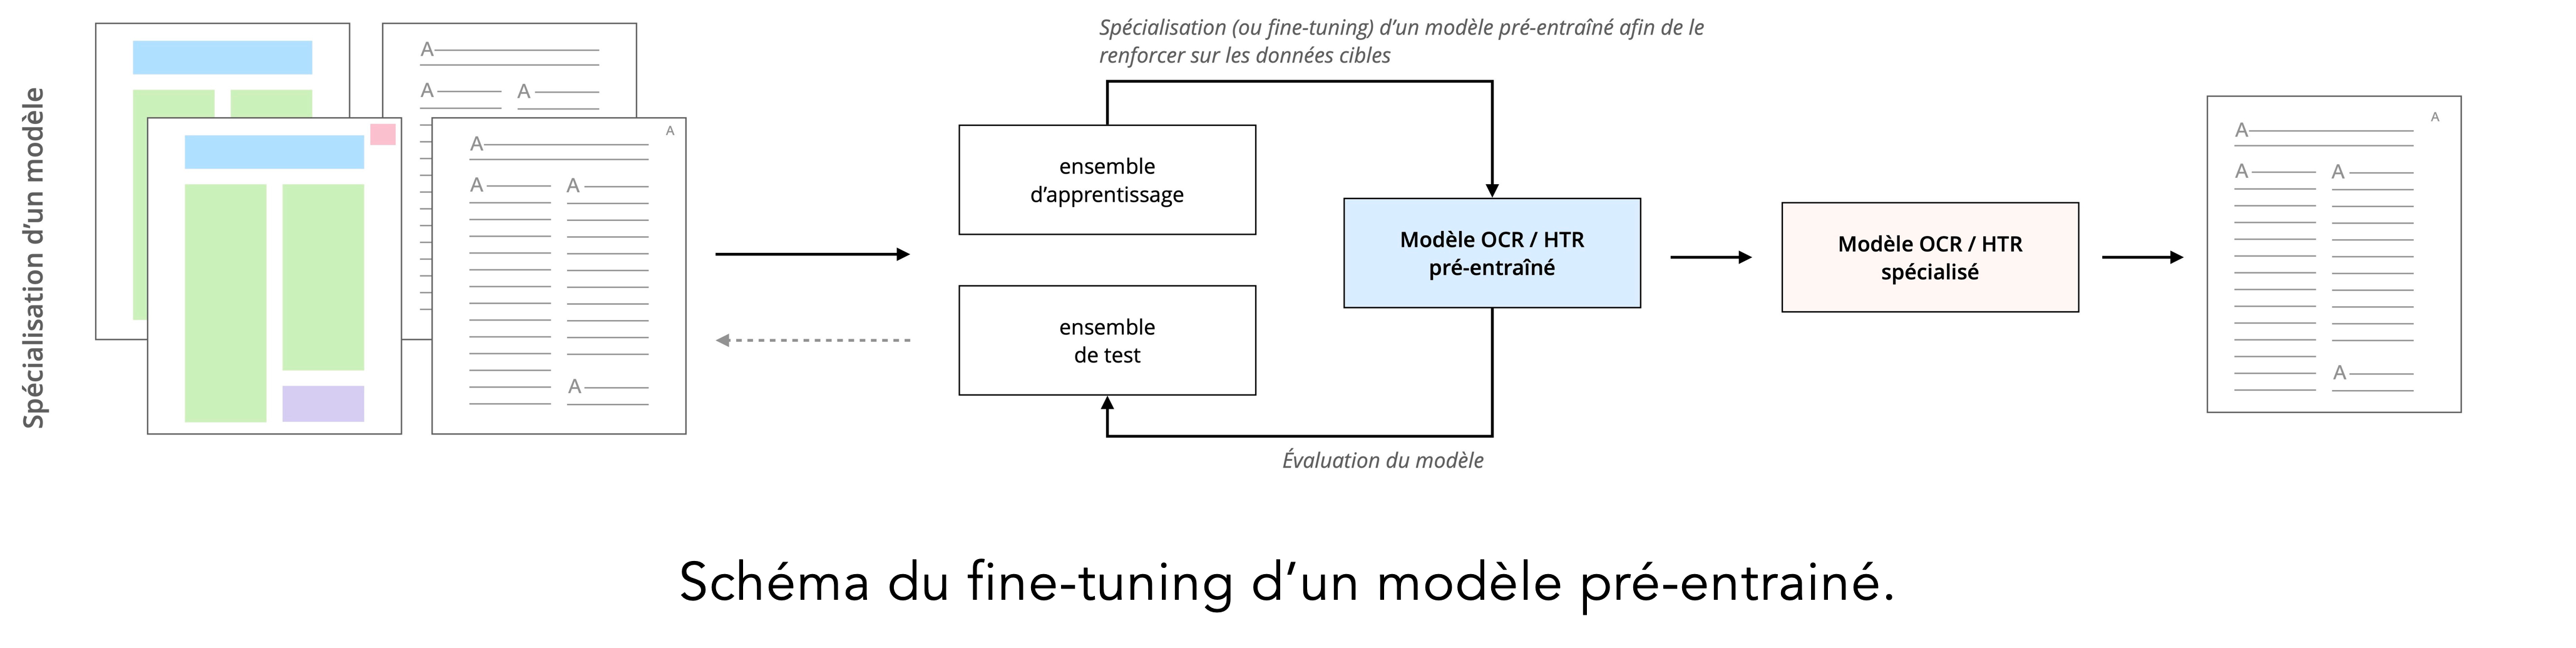
\includegraphics[width=0.8\textwidth]{images/schem_pretrain.png}
		\caption{Schéma du fine-tuning d’un modèle pré-entrainé. }
		\label{fig:monimage}
	\end{figure}
	
	Le fine-tuning est reconnu comme une méthode particulièrement efficace pour adapter les modèles de reconnaissance de texte manuscrit aux spécificités d’un corpus, surtout dans des contextes où les données sont hétérogènes et diversifiées, comme c’est le cas avec le corpus manuscrits de la BnF. En permettant d’affiner un modèle générique pré-entraîné à l’aide d’un petit ensemble de nouvelles données, le fine-tuning améliore la précision du modèle pour des tâches spécifiques, tout en optimisant les ressources et le temps nécessaires.
	\\
	
	Le principal avantage de cette méthode réside dans l’amélioration significative de la précision. Cette technique est idéale pour des institutions comme la BnF, qui possèdent des collections variées de manuscrits. Par exemple, le fine-tuning permet d’atteindre une précision supérieure à 98 \% avec un minimum de données supplémentaires, en adaptant efficacement un modèle générique aux particularités des manuscrits historiques\footcite{pinche_htr_2022}. Cette précision accrue est essentielle dans un contexte où la qualité de la transcription peut varier en fonction de la complexité des documents traités. De plus, le fine-tuning se distingue par son efficacité économique. Adapter un modèle générique via cette méthode est moins coûteux en termes de ressources et de temps que de développer un modèle de zéro. Cette approche est particulièrement avantageuse pour les projets de grande envergure menés par des établissements patrimoniaux, car elle permet d’améliorer significativement les performances des modèles avec un investissement minimal en données nouvelles.
	
	Le fine-tuning offre également une grande adaptabilité, permettant de personnaliser les modèles HTR en fonction des caractéristiques spécifiques des manuscrits. Cela est particulièrement pertinent pour des documents historiques où la variation de l’écriture est fréquente\footcite{pippi_how_2023}. Par exemple, cette technique s’avère très efficace pour adapter des modèles à des collections manuscrites d’un seul auteur ou d’un style particulier, améliorant ainsi la précision de la transcription.
	\\
	
	En outre, le fine-tuning contribue à la réduction des taux d’erreur. Même avec un nombre limité de lignes de texte annotées, cette méthode peut significativement diminuer le taux d’erreur de caractère, prouvant son efficacité pour améliorer les résultats de reconnaissance, même lorsque les données disponibles sont restreintes\footcite{kohut_finetuning_2023}.
	\\
	
	Cependant, le fine-tuning présente aussi certaines limites. Il dépend fortement de la qualité des données de base utilisées pour le pré-entraînement. Si le modèle générique est mal adapté dès le départ, le fine-tuning pourrait ne pas suffire à atteindre une précision optimale. De plus, un fine-tuning sur un petit ensemble de données spécifiques peut entraîner un risque de surapprentissage, où le modèle devient trop spécialisé et perd de sa généralité. Enfin, la mise en œuvre efficace du fine-tuning nécessite une expertise technique pour sélectionner les modèles pré-entraînés adéquats et optimiser les paramètres d’entraînement, ce qui pourrait impliquer un investissement supplémentaire pour des institutions comme la BnF.
	\\
	
	En somme, le fine-tuning se présente comme une solution puissante pour adapter des modèles HTR génériques à des corpus spécifiques, offrant une amélioration significative de la précision tout en étant économiquement avantageux. Néanmoins, cette méthode doit être utilisée avec précaution pour éviter les pièges du surapprentissage et garantir que le modèle générique de départ est bien adapté aux tâches envisagées. 
	
	Et nous pouvons donc nous demander si l’adoption de cette méthode, le fine-tuning, pour la reconnaissance manuscrite à la BnF représente une bonne stratégie afin de pouvoir traiter correctement la collection de manuscrits. Aux premier abord, cela peut paraître être une stratégie prometteuse afin de surmonter les défis liés à la diversité et à la complexité de ses vastes collections, en permettant l’adaptation rapide et précises des modèles génériques aux spécificités des documents conservés. De plus, le fine-tuning est une option qui offre une flexibilité indispensable pour traiter efficacement un large éventail de manuscrits, allant des textes médiévaux aux documents plus modernes. 
	\\
	
	Néanmoins, la mise en place de cette méthode nécessite une approche réfléchie. La BnF devra veiller à sélectionner des modèles pré-entraînés de haute qualité et à disposer des ressources techniques nécessaires pour effectuer un fine-tuning optimisé. Bien que cette technique puisse réduire les coûts et le temps associés à la transcription, elle n’est pas exempte de risques, notamment celui de surapprentissage, qui pourrait limiter la généralité des modèles pour d’autres types de documents. Un autre enjeu important concerne la question de la gestion du fine-tuning lui-même. Cette tâche est méthodique et requiert des compétences spécifiques en machine learning pour garantir un modèle optimal. Cela soulève un problème humain que la BnF devra résoudre, soit en recrutant des ingénieurs spécialisés, soit en externalisant cette expertise, ou encore en lançant des appels à projets. Cependant, en intégrant le fine-tuning de manière stratégique, la BnF pourrait non seulement améliorer la précision de ses transcriptions, mais aussi renforcer la valorisation et l’accessibilité de son patrimoine documentaire. 
	
	\subsection{Quel.s modèle.s pour les manuscrits de la BnF ?}
	
	Suite à ce grand tour des modèles et à cette réflexion sur le fine-tuning, la question se pose : dans le cadre de la mise en place d’un pipeline pour une chaîne HTR, quel modèle serait le plus approprié pour produire des résultats satisfaisants ? La BnF ne vise pas une reconnaissance parfaite de ses manuscrits, comme un taux de 99,98 \% requis pour des projets éditoriaux, ni même un taux de 90 à 95 \% que l’on peut atteindre avec l’OCR/HTR sur des imprimés anciens et contemporains. Ces niveaux de précision, bien que souhaitables, ne sont pas d’une utilité immédiate pour les objectifs actuels de la bibliothèque.
	\\
	
	La première option pour la BnF serait donc de recourir à des modèles génériques. Comme nous l’avons vu, ces modèles fournissent des résultats intéressants, que ce soit sur les ensembles d’entraînement ou sur un échantillon des manuscrits de la BnF. Ils représentent une base solide pour la transcription. Cependant, ces modèles présentent des limites notables en ce qui concerne les langues peu ou non représentées dans les corpus d’entraînement, comme l’arabe ou l’arménien, qui posent des défis spécifiques en raison de leur faible représentation dans les modèles HTR génériques existants.
	
	C’est dans ce contexte que des projets comme READ\_CHINESE, ainsi que le projet de la collection Dulaurier de la BnF sur l’arménien ancien, ont vu le jour. Ces initiatives visent à développer des modèles HTR spécialisés pour des langues complexes telles que le chinois, l’arabe ou l’arménien. Ces projets montrent qu’il est non seulement possible, mais également nécessaire de créer des modèles spécifiques pour répondre aux particularités linguistiques et scripturales de certains corpus.
	\\
	
	Face à la question du choix des modèles HTR pour la BnF, la réponse semble logiquement pencher en faveur des moteurs génériques, qui permettent de traiter une grande partie des manuscrits de la BnF, principalement composés de langues romanes comme le latin et le français, et couvrant de larges périodes. Toutefois, la possibilité d’une approche hybride ne doit pas être écartée. Utiliser des modèles génériques pour les langues et écritures bien représentées, tout en investissant dans le fine-tuning ou la création de modèles spécifiques pour les langues sous-représentées, pourrait être une stratégie judicieuse. Cette approche permettrait de couvrir un éventail plus large de documents, tout en garantissant une qualité de transcription suffisante pour les besoins de la BnF, même si l’objectif n’est pas d’atteindre une précision éditoriale parfaite.
	\\
	
	En somme, pour la BnF, la mise en place d’une chaîne HTR efficace pourrait passer par une combinaison de modèles génériques et spécifiques, adaptée aux particularités des collections qu’elle souhaite transcrire. Cette approche permettrait de surmonter les limitations actuelles liées aux langues sous-représentées et d’assurer une couverture plus exhaustive de son vaste patrimoine manuscrit.
	
	\part{Conclusion}
	\chapter*{Conclusion}
	\addcontentsline{toc}{chapter}{Conclusion}
	
	Ce mémoire a cherché à répondre à la question centrale : Quels sont les principaux défis de la mise en place d’un projet d’intelligence artificielle à échelle industrielle dans le domaine patrimonial, et comment peuvent-ils être surmontés au sein d’une institution comme la Bibliothèque nationale de France ? L’analyse a montré que l’intégration de technologies comme la reconnaissance de texte manuscrit nécessite non seulement des avancées techniques, mais aussi une organisation méticuleuse et une collaboration étroite entre différents départements et partenaires externes afin de faire avancer la technologie.
	\\
	
	Les défis sont multiples : ils concernent la diversité des manuscrits, la qualité et la normalisation des métadonnées, ainsi que la nécessité de développer des modèles spécifiques adaptés aux particularités des documents patrimoniaux. Pour surmonter ces obstacles, une approche intégrée, combinant expertise technique, gestion rigoureuse des données et innovation continue, s’avère essentielle. Mon stage au sein du service de numérisation de la BnF a permis de confronter ces enjeux théoriques à la réalité du terrain. La mise en place d’un pipeline HTR, bien que complexe, a révélé l’importance d’une préparation minutieuse des données et d’une collaboration interdisciplinaire pour garantir la réussite du projet. Les résultats obtenus, bien que limités par les contraintes de temps et de ressources, ouvrent la voie à des améliorations futures, notamment par l’affinement des modèles et la poursuite des collaborations avec des experts en intelligence artificielle.
	\\
	
	En conclusion, l'intégration de l'intelligence artificielle dans le domaine patrimonial représente un véritable changement de paradigme, offrant de nouvelles perspectives pour la conservation et la valorisation des collections. Cette transformation nécessite une réflexion stratégique et des ressources adaptées pour en maximiser les bénéfices tout en respectant les spécificités du patrimoine. La BnF, en tant qu'institution pionnière, est bien placée pour relever ces défis et continuer à innover dans ce domaine. À long terme, ces avancées pourraient non seulement améliorer l'accessibilité des documents historiques, mais aussi ouvrir de nouvelles voies pour la recherche en sciences humaines et sociales, en permettant des analyses à grande échelle de textes manuscrits jusqu'alors difficilement exploitables.
	
	
	
\newpage{\pagestyle{empty}\cleardoublepage}







%%%%%%%%%%%%%%%%%%

\appendix %Des appendices: tables figures, etc
\chapter{Figures.}
Ces présents documents servent à appuyer et illustrer les propos présents dans ce mémoire afin de faciliter la compréhension des exemples ou des affirmations.

\begin{figure}
	\centering
	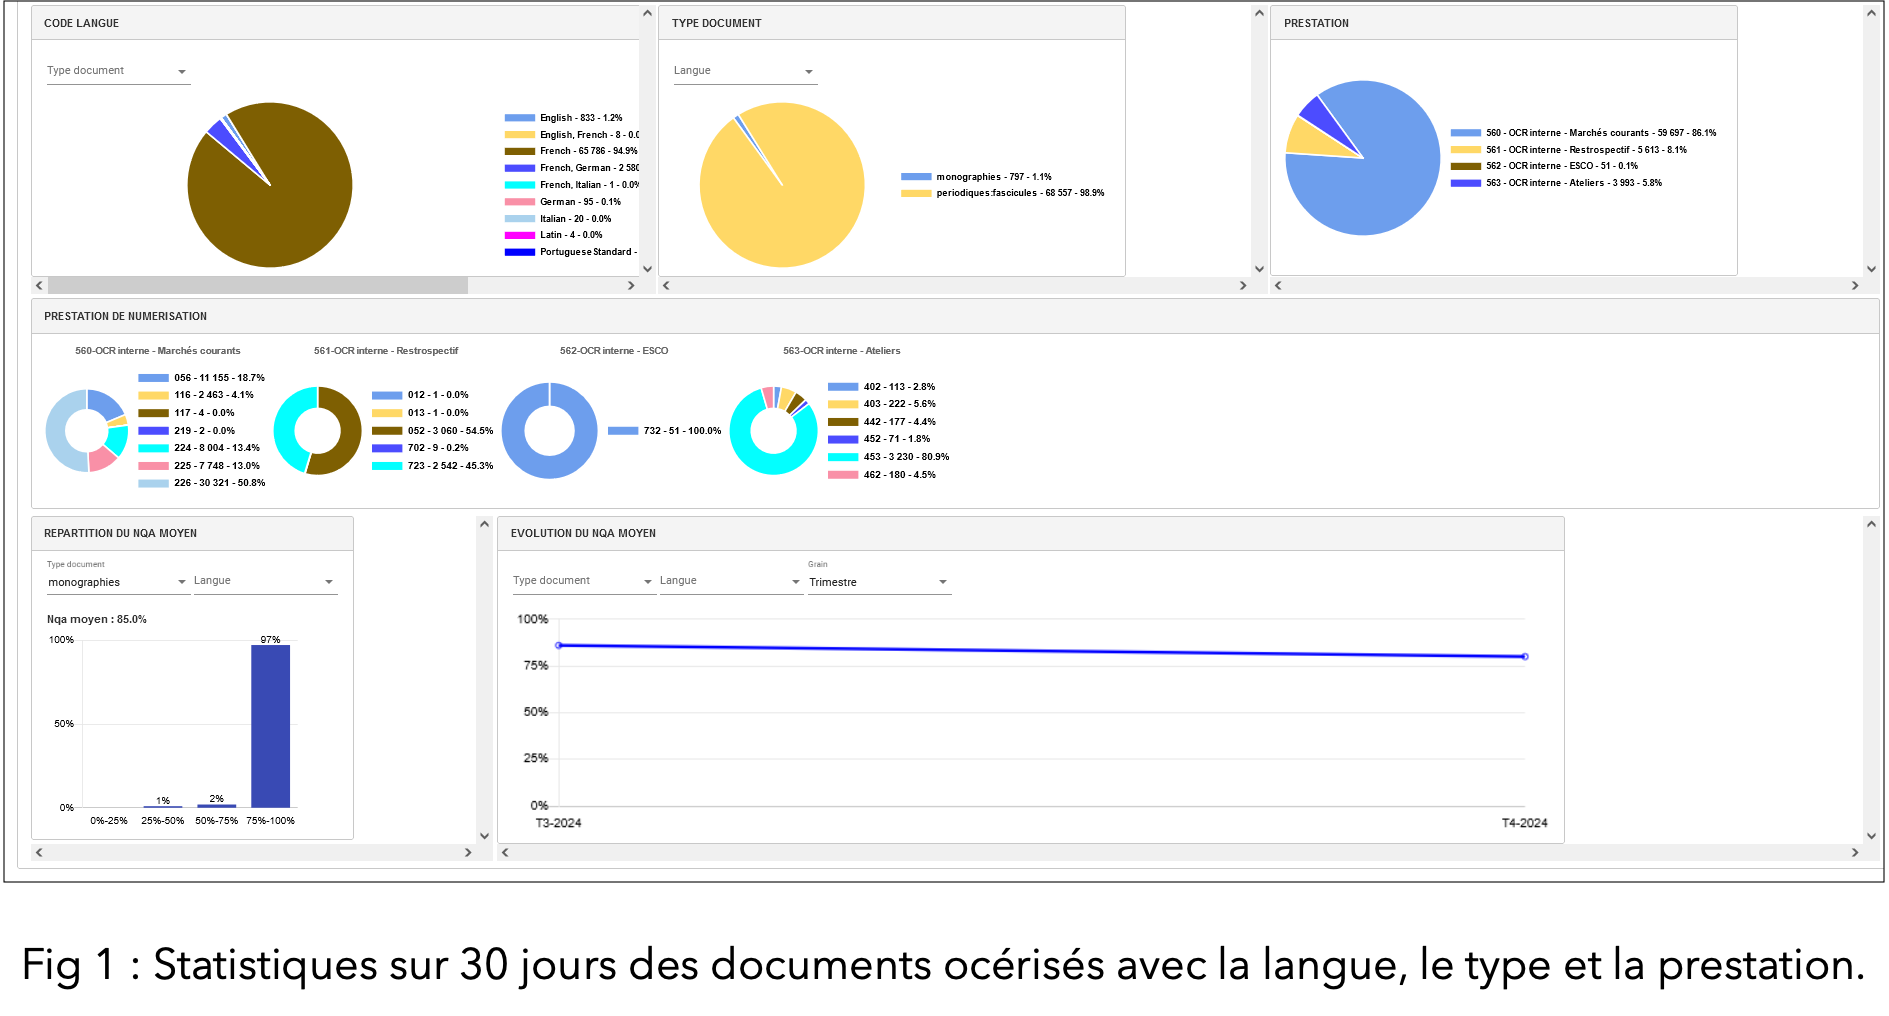
\includegraphics[width=0.7\linewidth]{images/stat_suivinum}
	\caption{Statistiques sur 30 jours des documents océrisés avec la langue, le type et la prestation.}
	\label{fig:statsuivinum}
\end{figure}

\begin{figure}
	\centering
	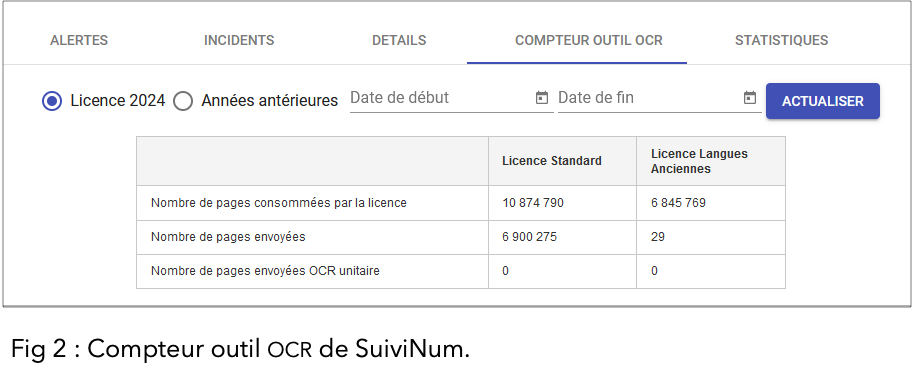
\includegraphics[width=0.7\linewidth]{images/compteur_ocr}
	\caption{Compteur outil OCR de SuiviNum}
	\label{fig:compteurocr}
\end{figure}

\begin{figure}
	\centering
	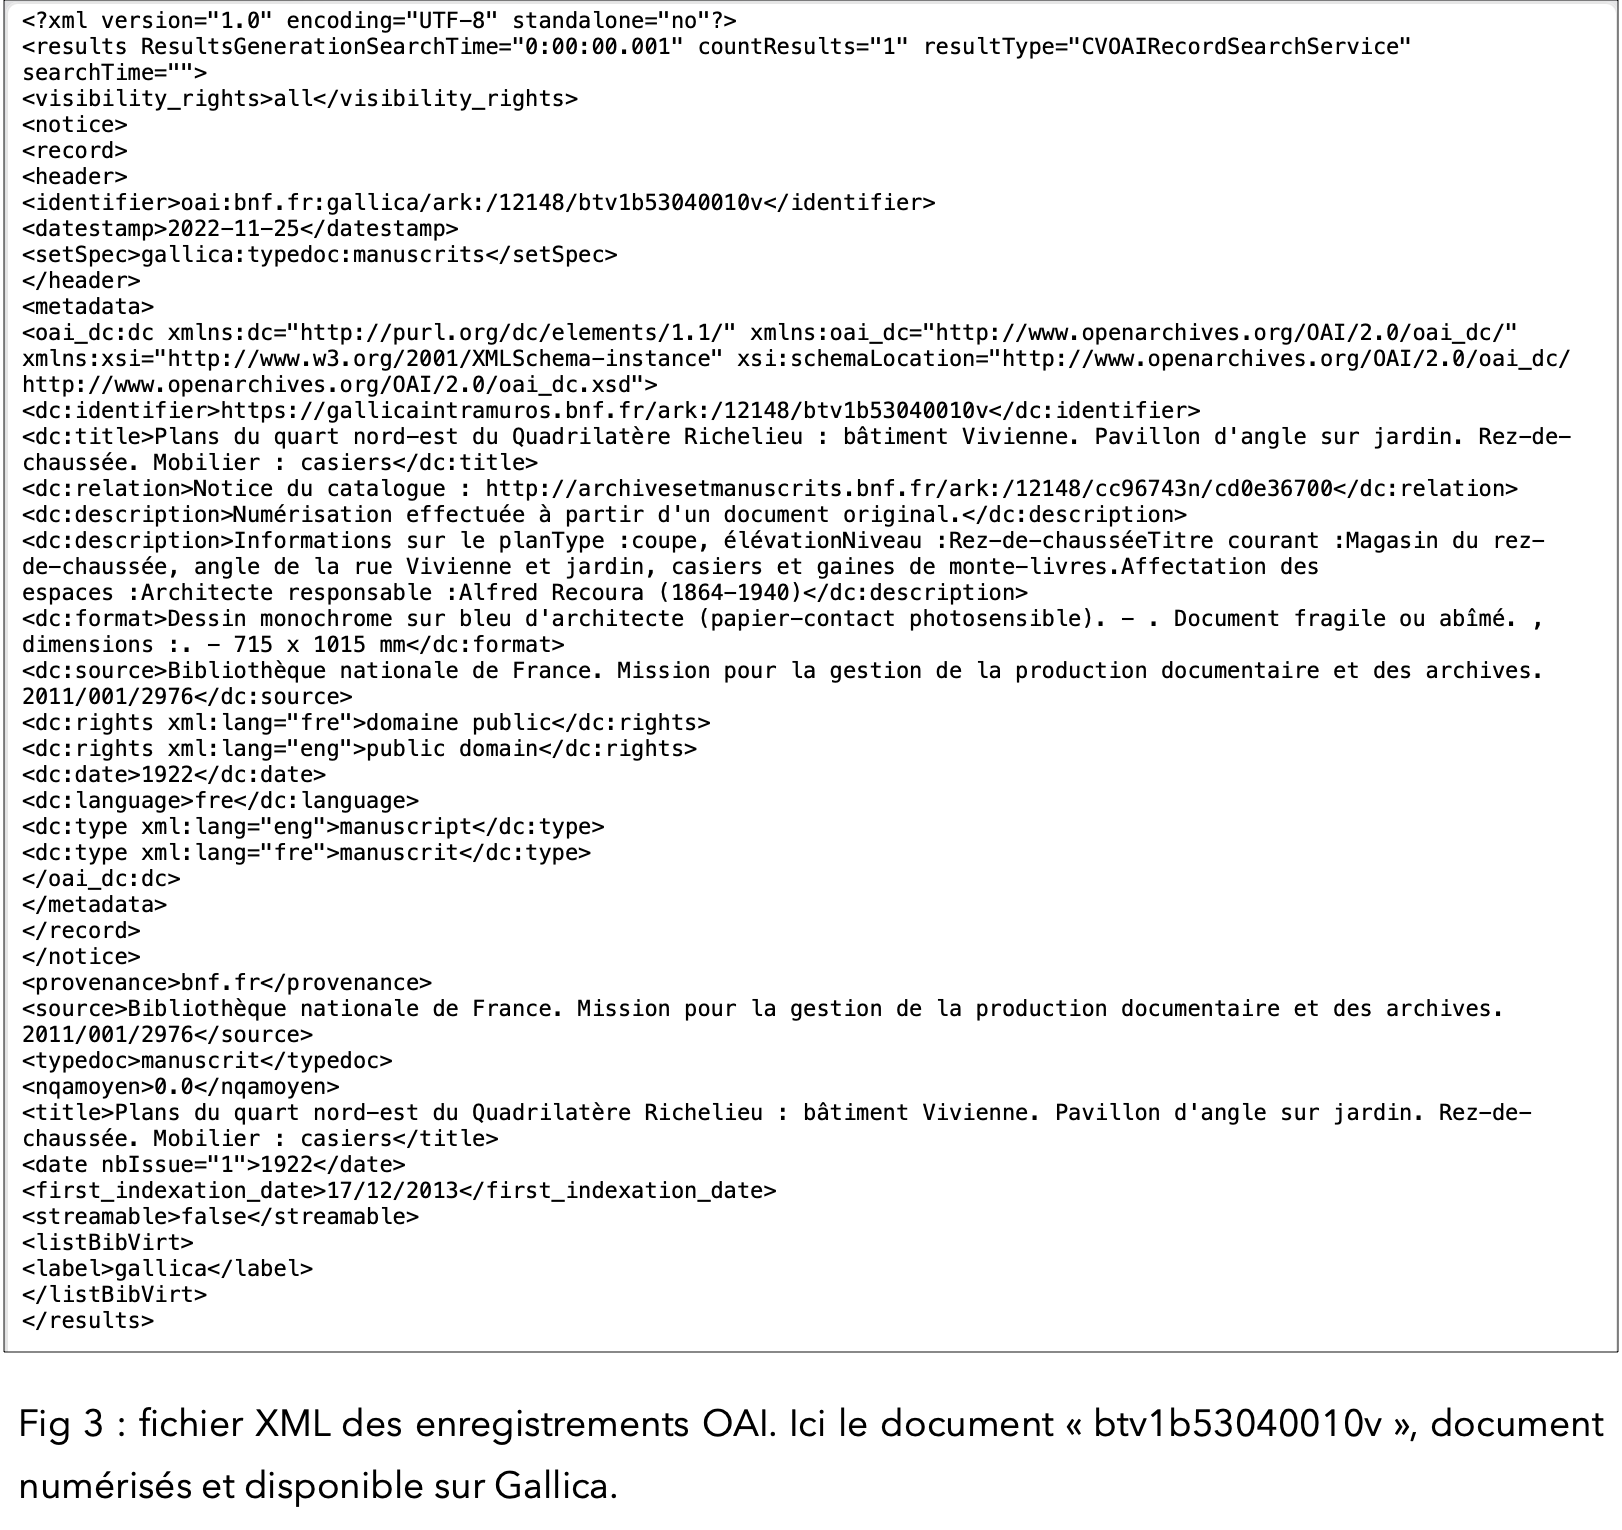
\includegraphics[width=0.7\linewidth]{images/fiche_xml_oai}
	\caption{Fichier XML des enregistrements OAI. Ici le document « btv1b53040010v », document numérisés et disponible sur Gallica.}
	\label{fig:fichexmloai}
\end{figure}

\begin{figure}
	\centering
	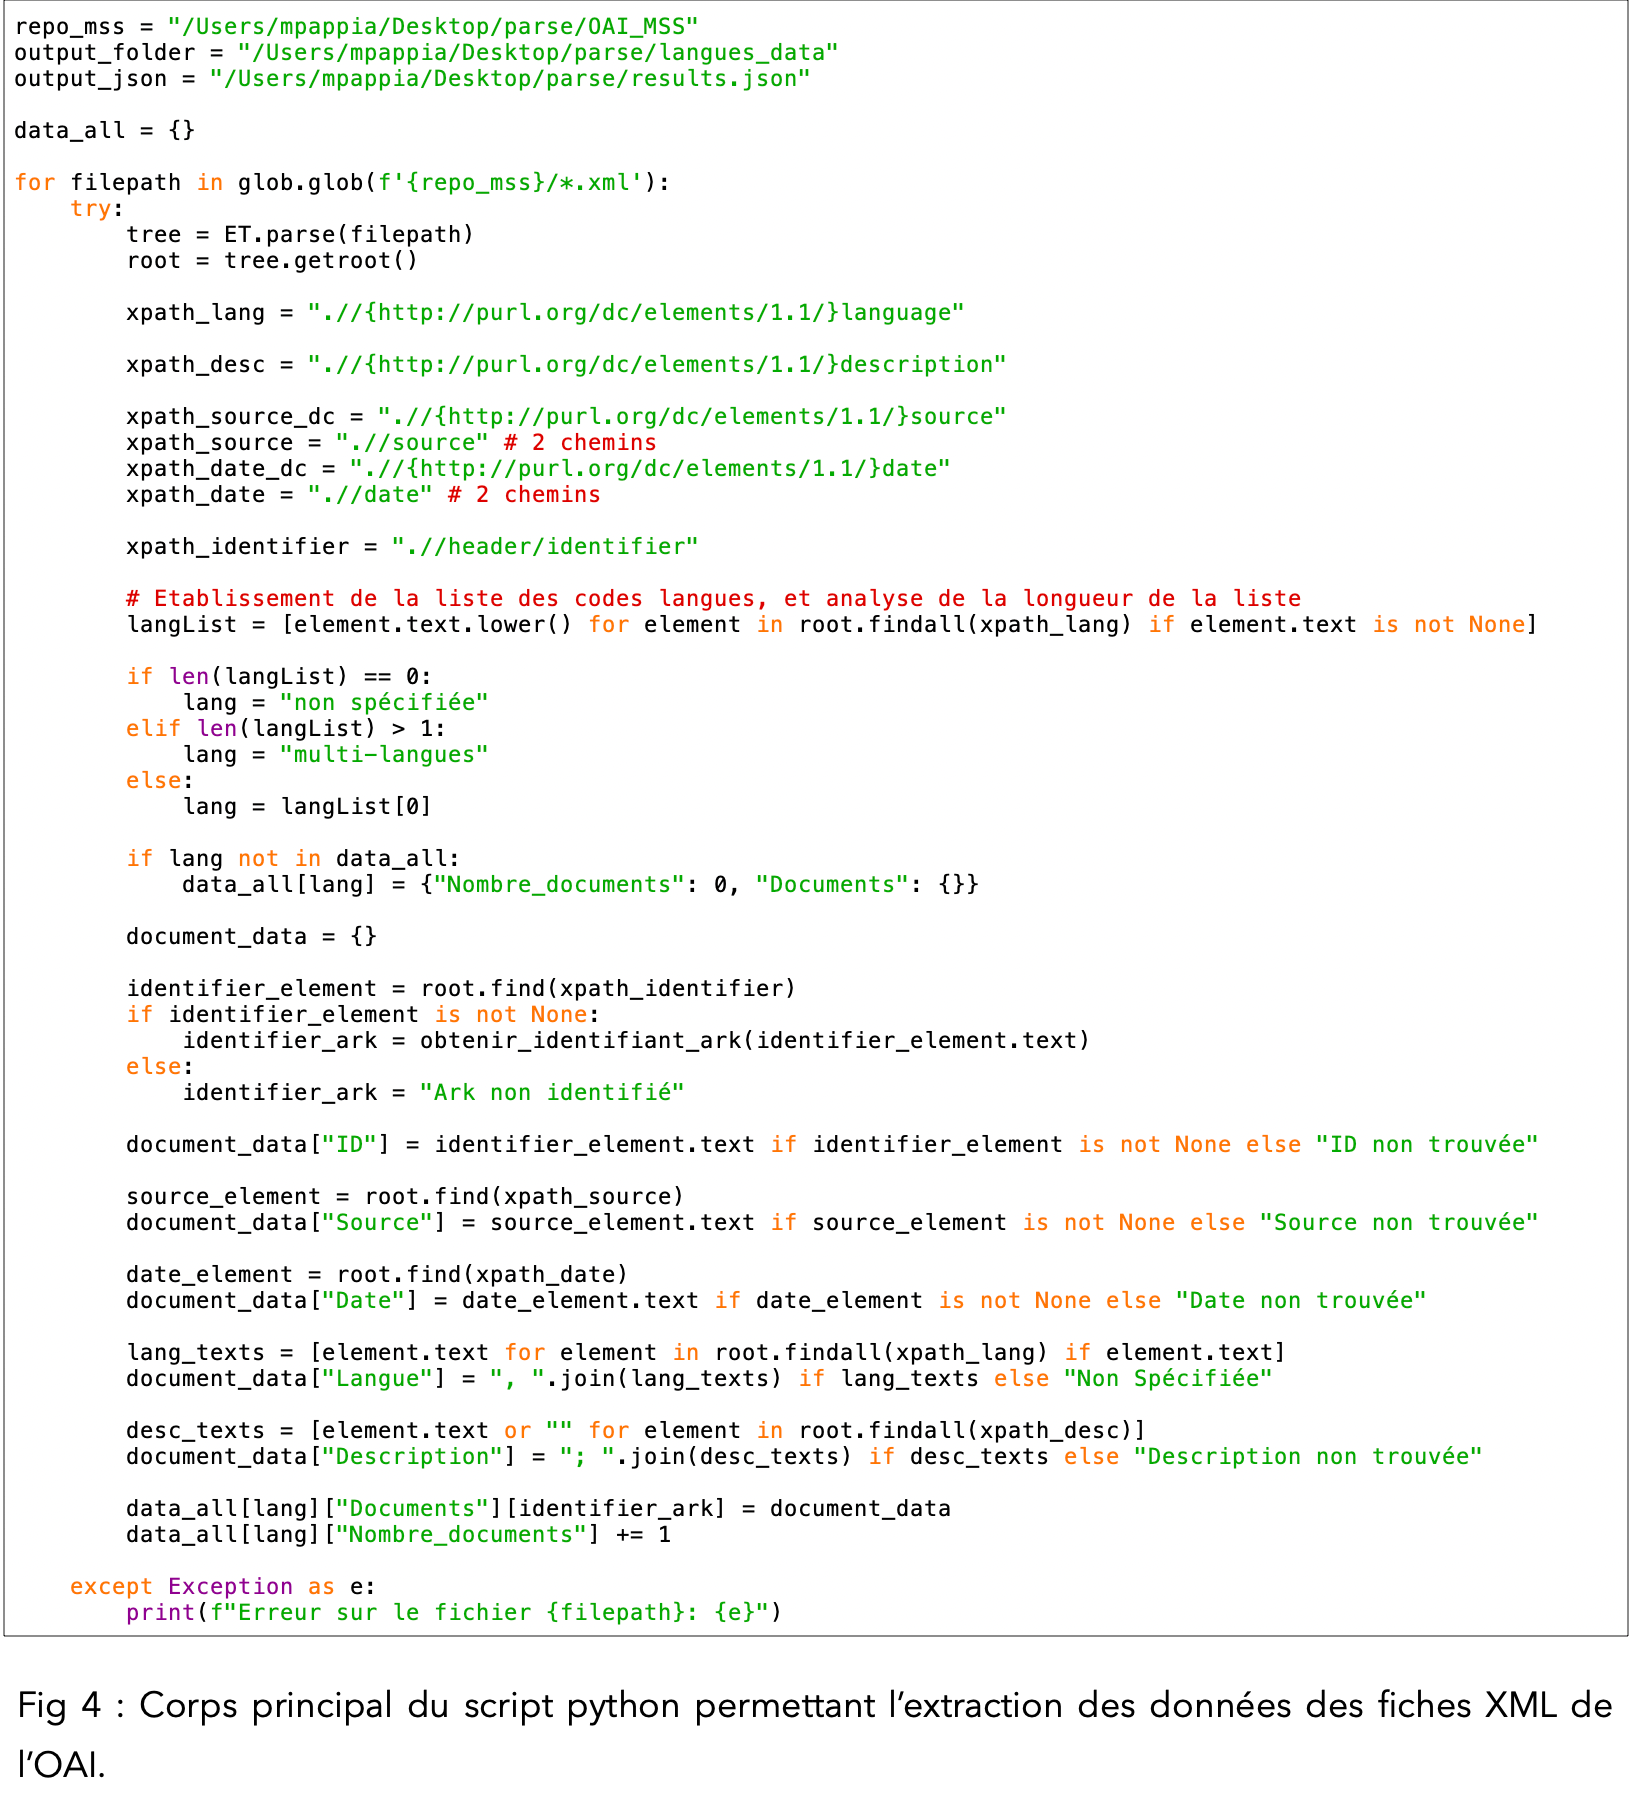
\includegraphics[width=0.7\linewidth]{images/script_python_a}
	\caption{Corps principal du script python permettant l’extraction des données des fiches XML de l’OAI.}
	\label{fig:scriptpythona}
\end{figure}

\begin{figure}
	\centering
	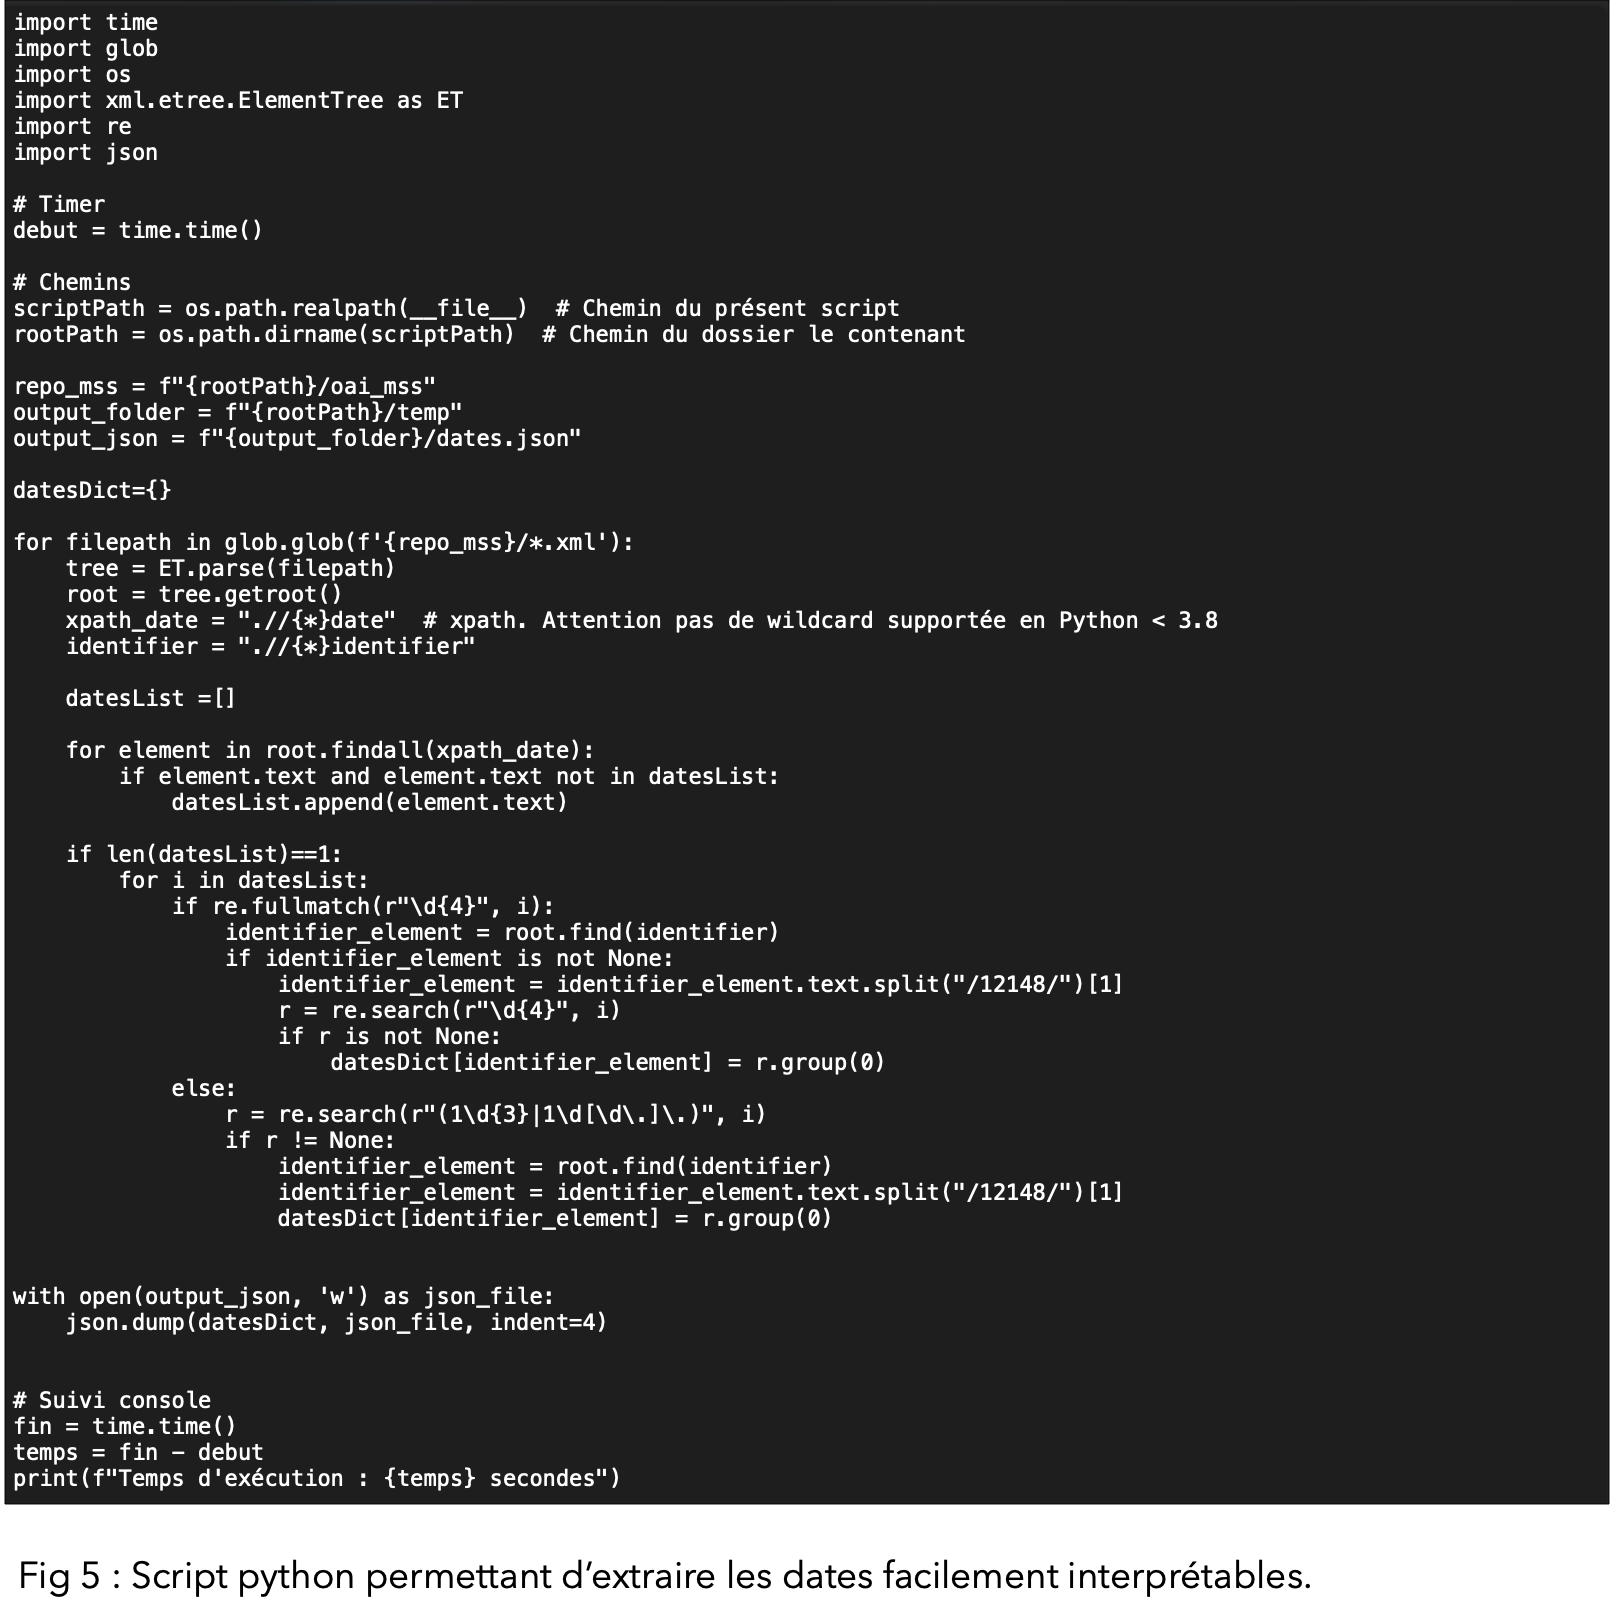
\includegraphics[width=0.7\linewidth]{images/script_python_b}
	\caption{Script python permettant d’extraire les dates facilement interprétables.}
	\label{fig:scriptpythonb}
\end{figure}

\begin{figure}
	\centering
	\includegraphics[width=0.7\linewidth]{images/segm_krak}
	\caption{Exemple de segmentation des lignes réalisé par le moteur, ici Kraken. }
	\label{fig:segmkrak}
\end{figure}

\begin{figure}
	\centering
	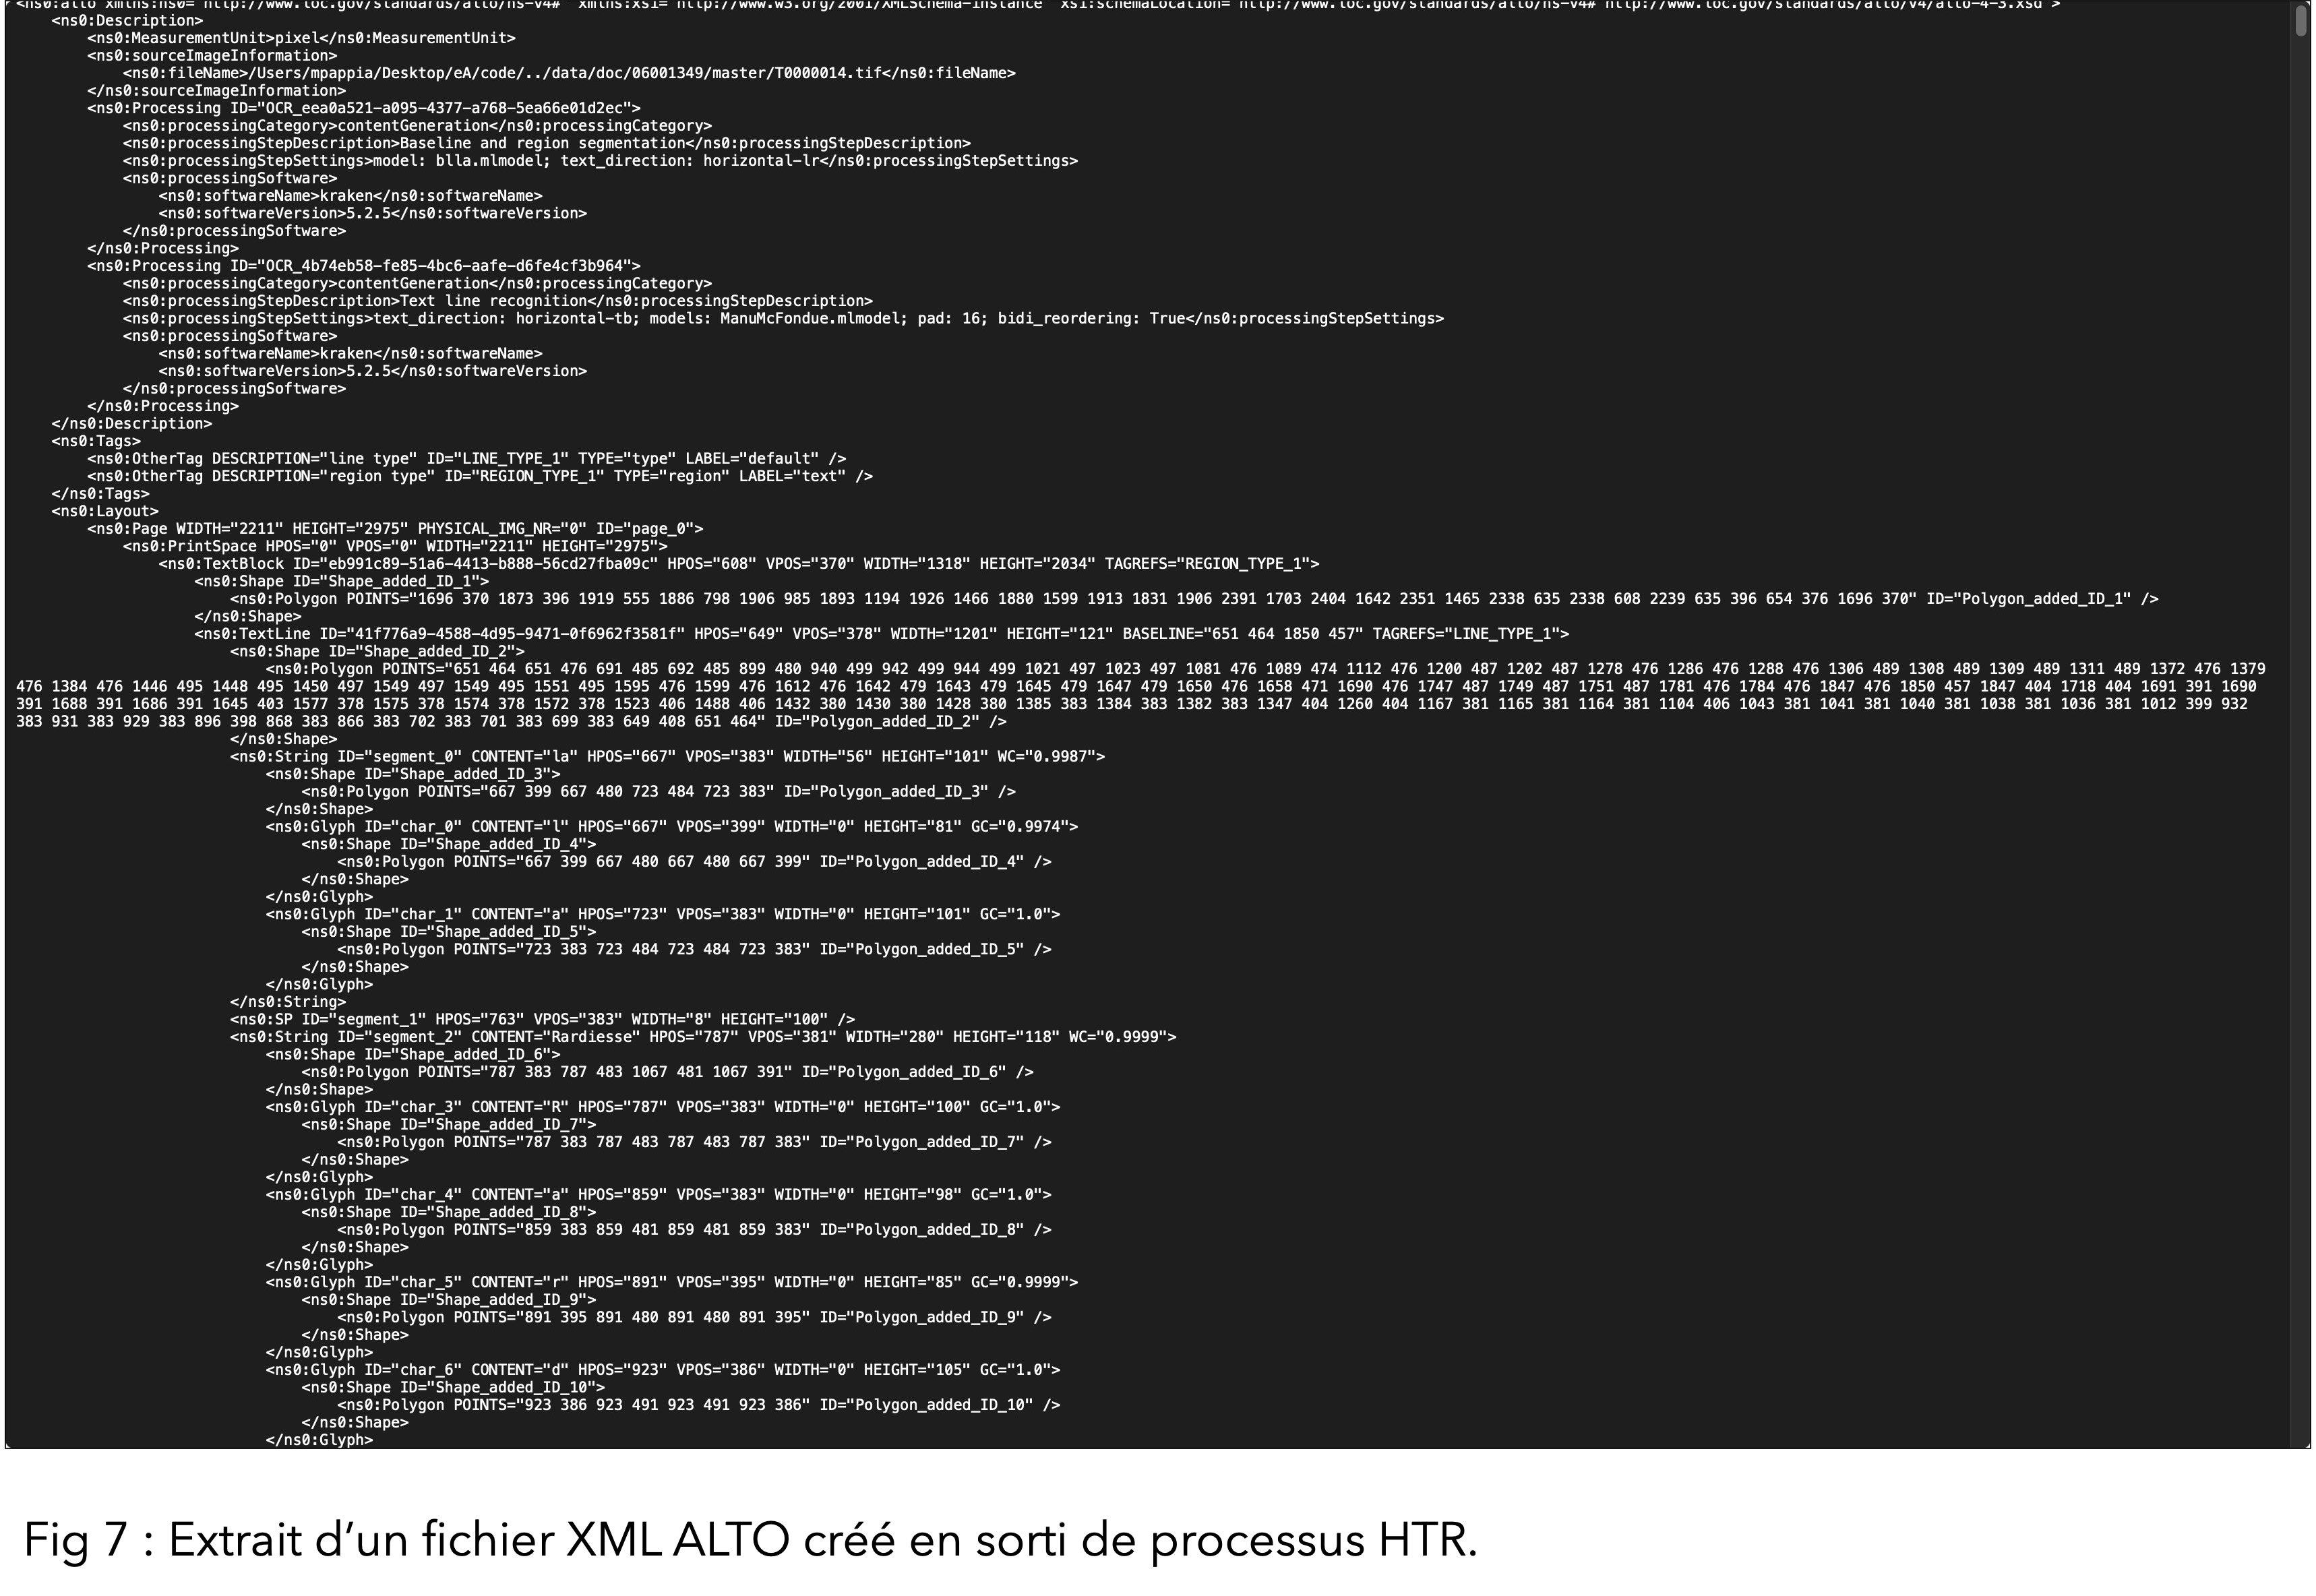
\includegraphics[width=0.7\linewidth]{images/ALTO_xml}
	\caption{Extrait d’un fichier XML ALTO créé en sorti de processus HTR.}
	\label{fig:altoxml}
\end{figure}


\begin{figure}
	\centering
	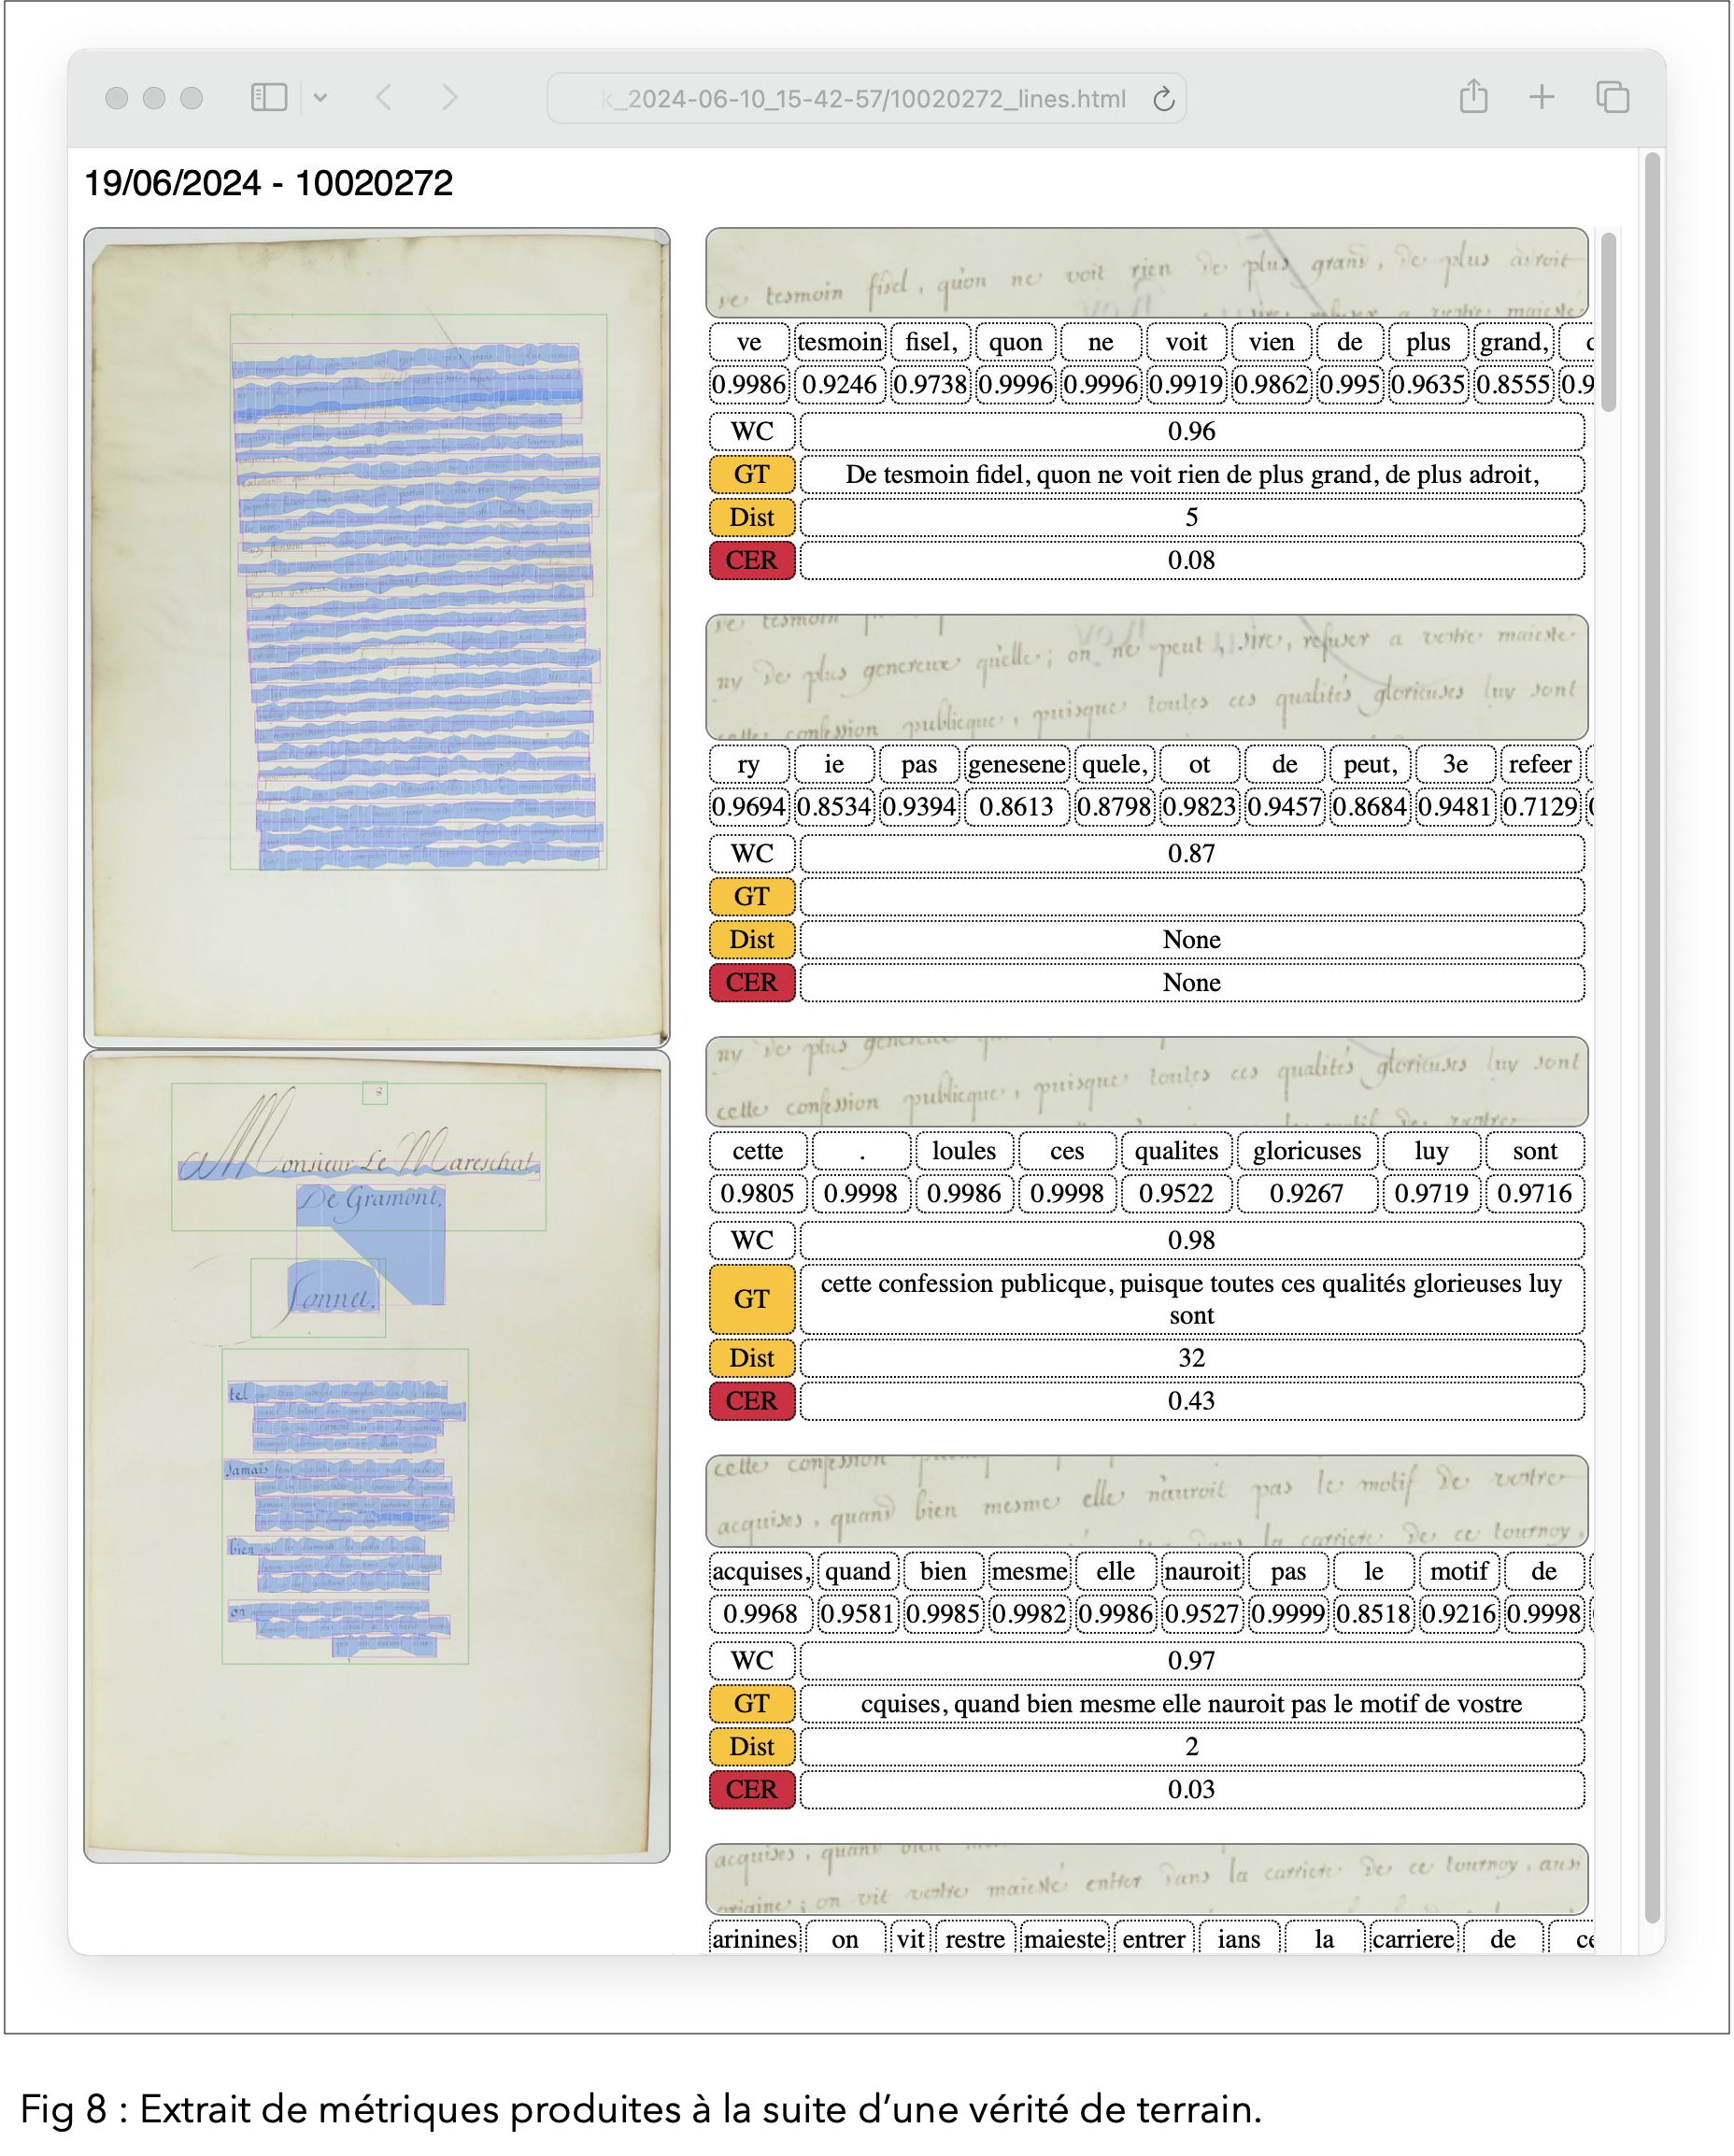
\includegraphics[width=0.7\linewidth]{images/verit_ter}
	\caption{Extrait de métriques produites à la suite d’une vérité de terrain.}
	\label{fig:veritter}
\end{figure}

\begin{figure}
	\centering
	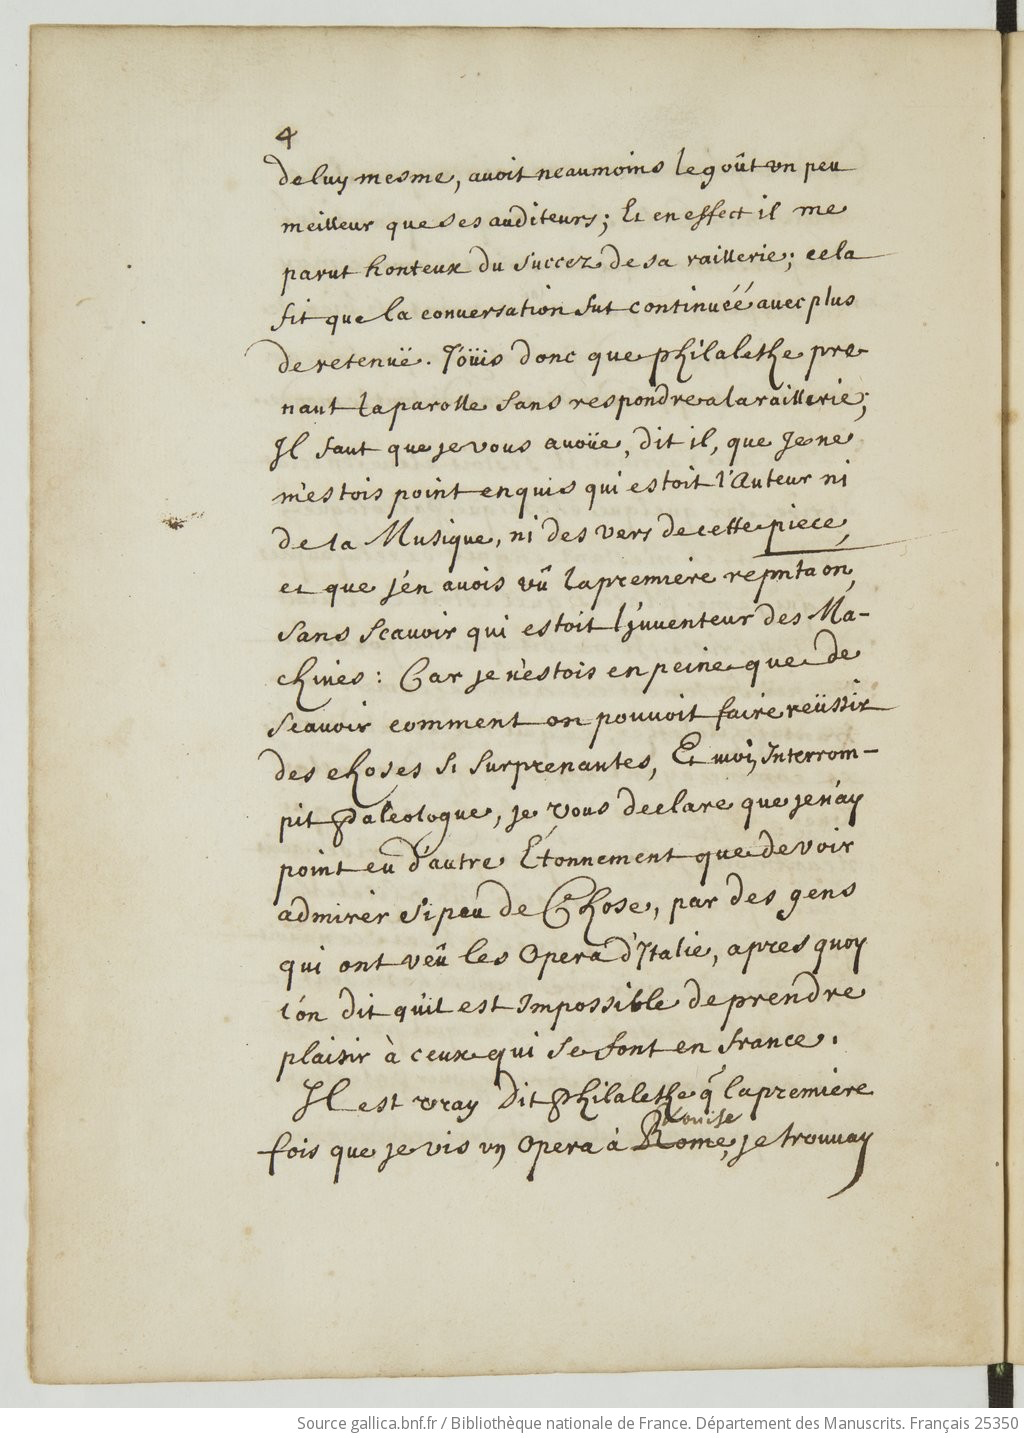
\includegraphics[width=0.7\linewidth]{images/mss_bnf_ex_1}
	\caption{Extrait du manuscrit btv1b525094323}
	\label{fig:mssbnfex1}
\end{figure}

\begin{figure}
	\centering
	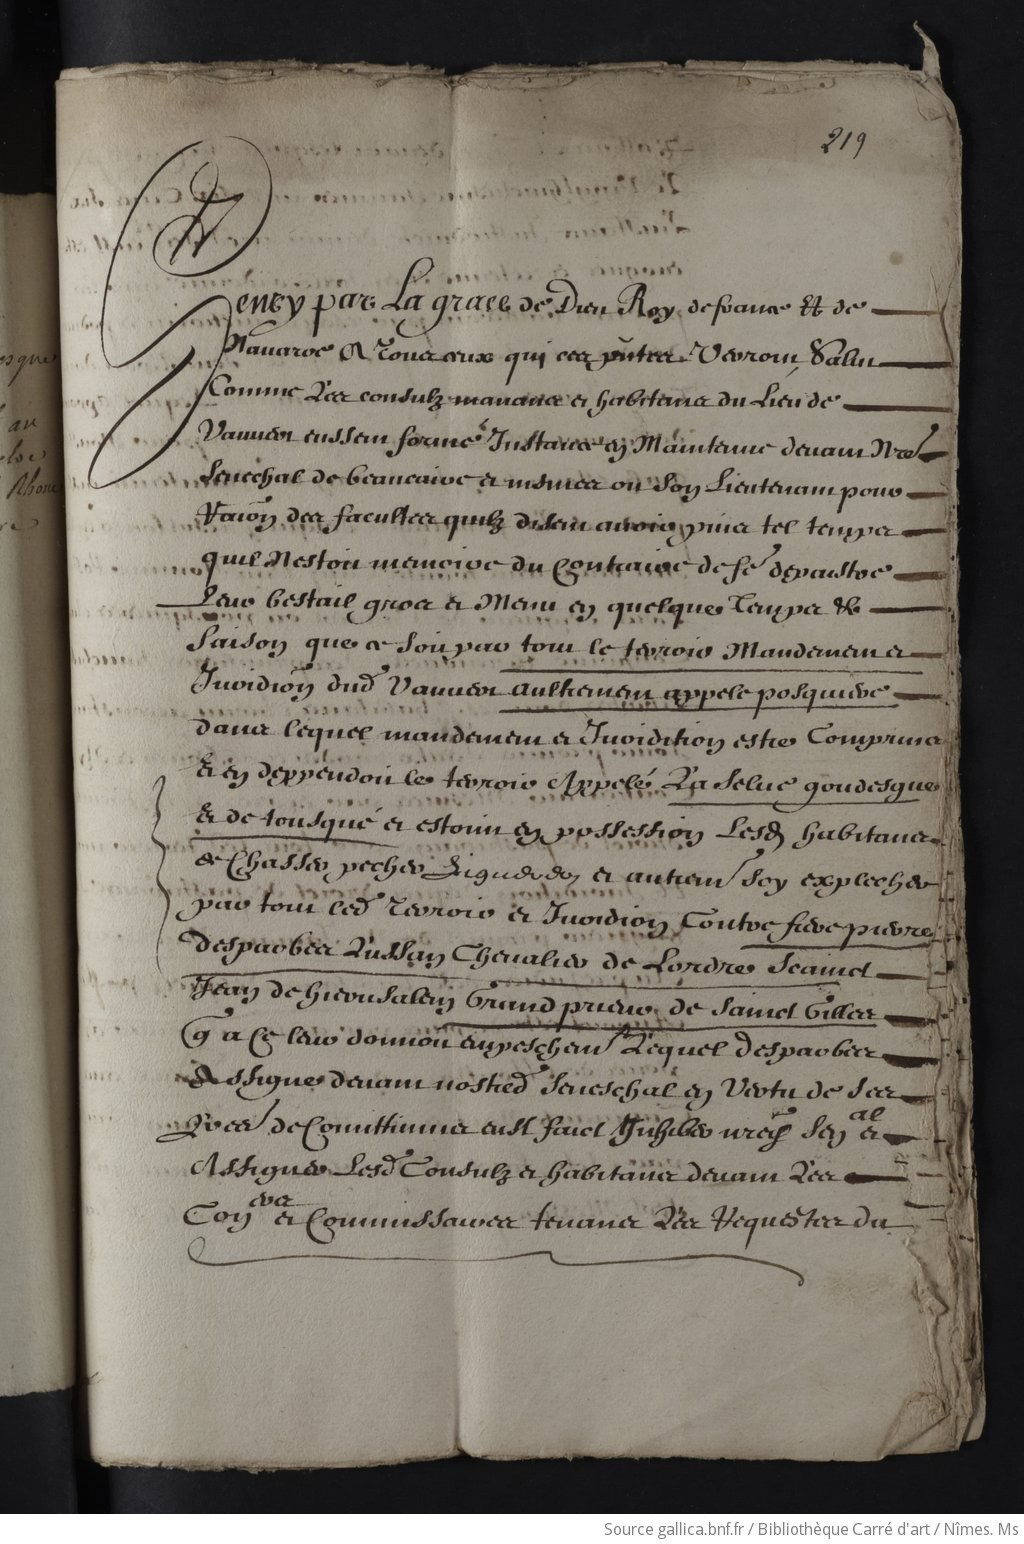
\includegraphics[width=0.7\linewidth]{images/mss_bnf_ex_2}
	\caption{Extrait du manuscrit btv1b10015954z}
	\label{fig:mssbnfex2}
\end{figure}

\begin{figure}
	\centering
	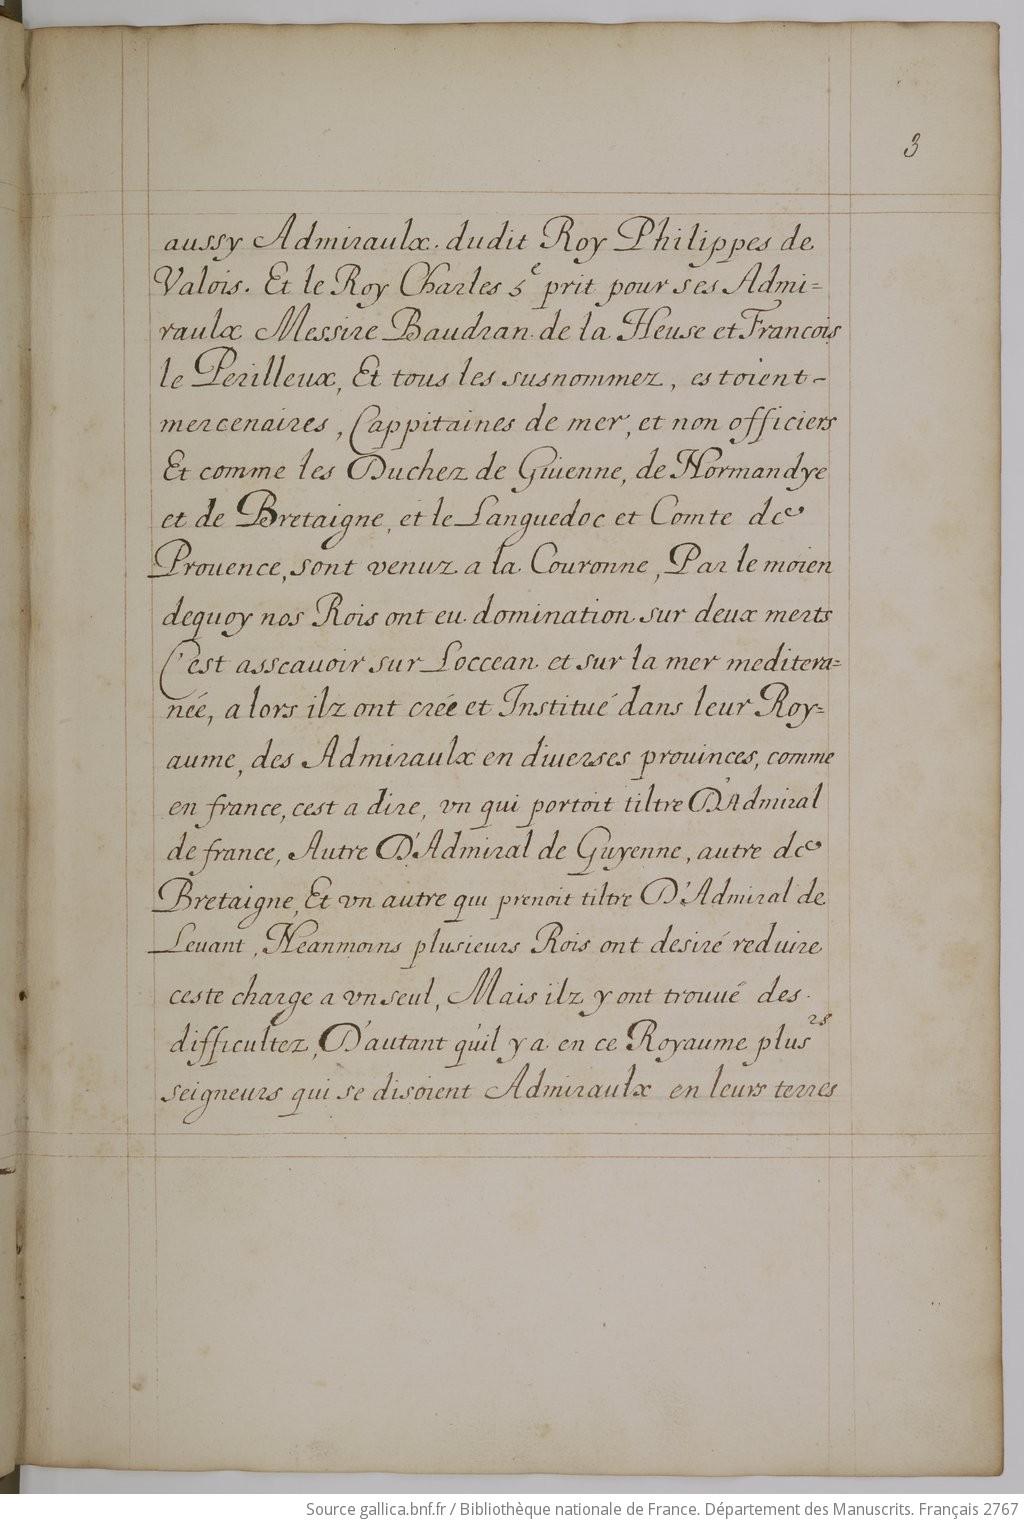
\includegraphics[width=0.7\linewidth]{images/exbnf3}
	\caption{Extrait du manuscrit btv1b84701789}
	\label{fig:mssbnfex3}
\end{figure}


\chapter{Les grands schémas de la BnF}
Ici sont présents des schémas de différents grands points abordés durant ce mémoire : Organisation de la BnF pour le fonctionnement de la chaîne OCR, Pipeline de l'OCR ainsi que de la chaîne d'entrée des documents numérisés.

\begin{figure}[h!]
	\centering
	\begin{minipage}{0.85\textwidth}
		\small
		Ce schéma illustre le processus organisationnel de la chaîne OCR à la BnF,  en décrivant les différentes étapes, depuis la phase de test et la numérisation jusqu’au contrôle qualité et au traitement OCR final.
	\end{minipage}
	\\
	\medskip
	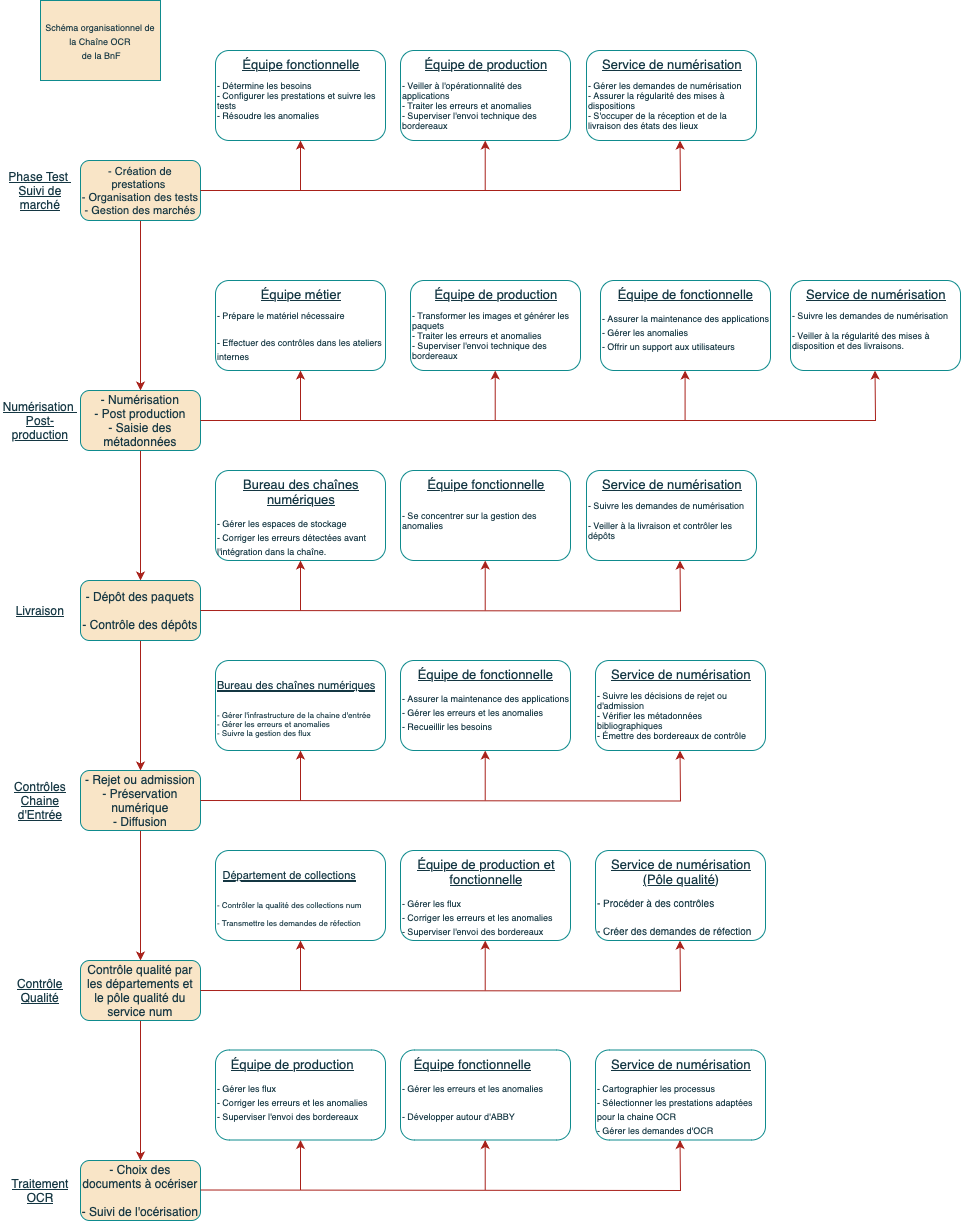
\includegraphics[width=0.7\linewidth]{images/schem_organ_bnf}
	\caption{Schéma organisationnel de la chaine OCR de la BnF}
	\label{fig:schemorganbnf}
\end{figure}

\begin{figure}
	\centering
	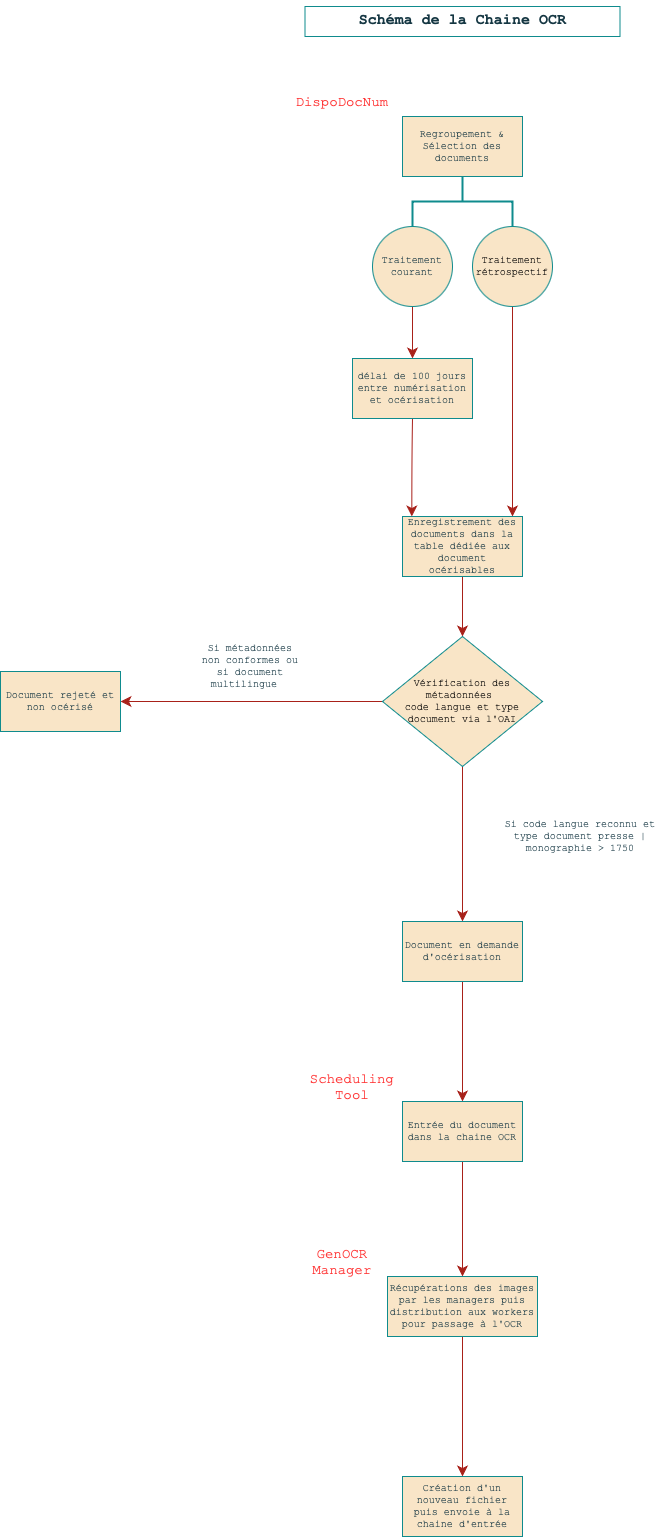
\includegraphics[width=0.7\linewidth]{images/schem_ocr_bnf}
	\caption{Schéma de la chaine OCR}
	\label{fig:schemocrbnf}
\end{figure}

\begin{figure}
	\centering
	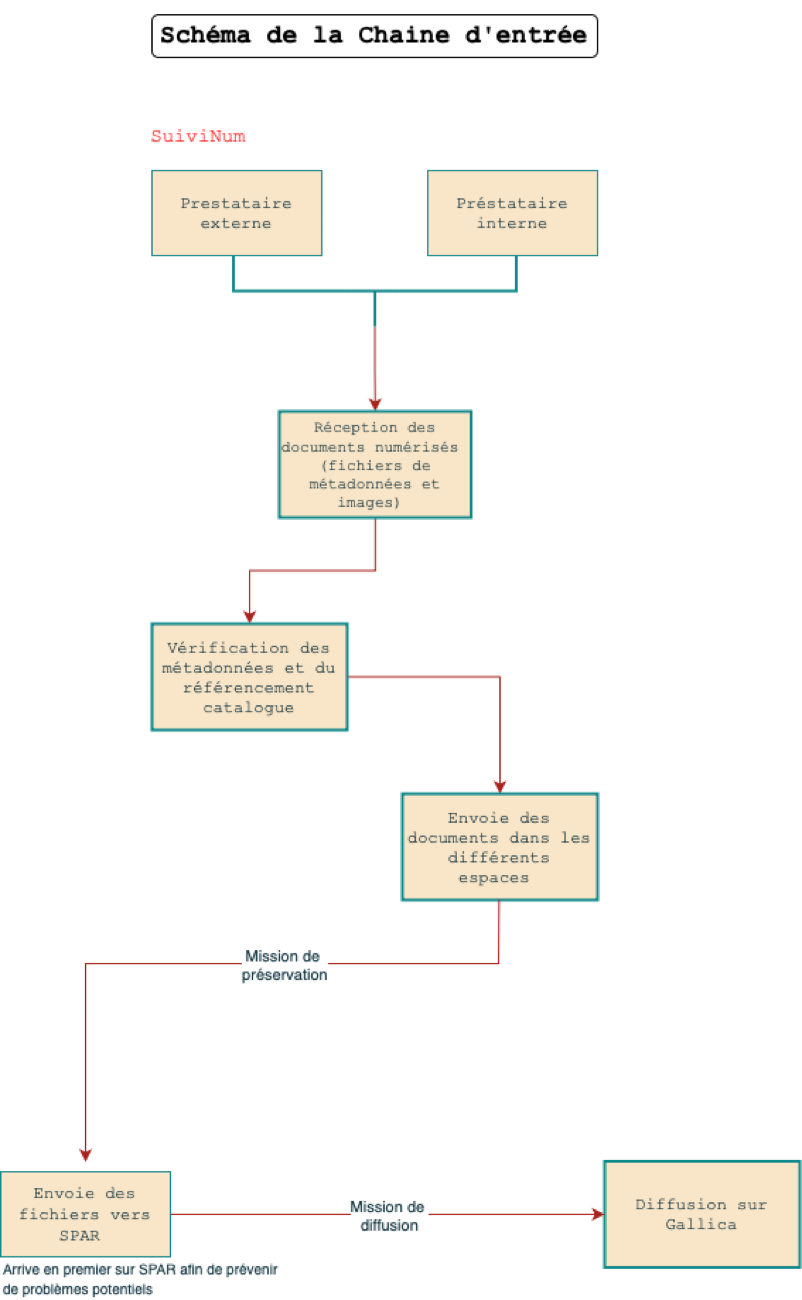
\includegraphics[width=0.7\linewidth]{images/schem_num_bnf}
	\caption{Schéma de la Chaine d’entrée des documents numérisés }
	\label{fig:schemnumbnf}
\end{figure}




\newpage{\pagestyle{empty}\cleardoublepage}

%%%%%%%%%%%%%%%%%%

\backmatter % glossaire, index, table des figures, table des matières.. (la bibliographie a déjà été appelée)

%\printindex
%\printglossaries[title=Glossaire]
%\listoftables
%\listoffigures
\tableofcontents
\end{document}
